
\chapter{Teoría intuitiva de Conjuntos}

\PartialToc

\hypersetup{linkcolor=ptctitle}

\vspace*{0.5cm}
 
\begin{flushright}
\textit{\footnotesize{}El principio de razón suficiente, que afirma
que nada}
\par\end{flushright}{\footnotesize \par}

\begin{flushright}
\textit{\footnotesize{}sucede gratuitamente, es decir, que a todo
fenómeno }
\par\end{flushright}{\footnotesize \par}

\begin{flushright}
\textit{\footnotesize{}le corresponde una explicación, una razón de
ser }
\par\end{flushright}{\footnotesize \par}

\begin{flushright}
\textit{\footnotesize{}que se presente admisible a la razón. }
\par\end{flushright}{\footnotesize \par}

\begin{flushright}
{\small{} }Leibniz: 
\par\end{flushright}

\vspace*{-1mm}

\begin{competencias}  \begin{lista}  

\item Interpreta correctamente los conceptos de conjunto y elemento. 

\item Argumenta los procedimientos para realizar operaciones entre
conjuntos . 

\item Maneja con criterio las operaciones y sus propiedades en los
diferentes sistemas numéricos.

\end{lista} \end{competencias}

\noindent

\begin{logros} 
\noindent
\begin{lista}  

\item Identifica conjuntos. 

\item Clasifica conjuntos. 

\item Realiza operaciones entre conjuntos.

\item Deduce las propiedades de los conjuntos a partir de los axiomas,
definiciones y otras propiedades.

\item Aplica bien las propiedades de los conjuntos.

\item Utiliza los diagramas de Venn para representar operaciones
y relaciones entre conjuntos. 

\end{lista} \end{logros}

\section{Introducción}

Este primer capítulo es una breve introducción a la lógica, que es
la herramienta que usan las matemáticas para desarrollarse.

El objetivo del mismo es describir en que consiste una teoría matemática.
Para lograrlo, primero hay que exponer sucintamente las reglas de
la lógica de proposiciones, definir con precisión que es un razonamiento
lógico y, por ultimo, explicar en que consiste una teoría matemática
(brevemente, una serie de axiomas, definiciones y teoremas relacionados
entre sí mediante argumentos lógicos, como veremos mas adelante). 

La lógica es un esquema de reglas que permite deducir verdades a partir
de o otras verdades. El medio que lleva de las primeras verdades a
las otras deducidas se llama razonamiento lógico. La lógica estudia,
precisamente, los razonamientos lógicos, estableciendo cuándo un razonamiento
es valido, independientemente del contenido de las verdades que se
enuncien. Sólo le interesan las manipulaciones que se hacen con los
enunciados, no su contenido.

Todos los resultados mostrados en este capítulo se prueban rigurosamente.
Sin embargo, no se usa para ello el razonamiento lógico, que que se
utiliza en un curso de lógica matemática sino el simple y eficaz camino
de las tablas introducidas en la sección \ref{sub:Relaciones-entre-proposiciones}
. Por supuesto, algunos resultados si se podrán demostrar a partir
de otros anteriores mediante las leyes del álgebra de proposiciones,
que se exponen en la a sección \ref{subsec:Operaciones-entre-proposiciones}.
Pero hemos preferido dejar todo el capítulo en manos de las tablas.

Por otra parte Uno de los aspectos fundamentales en cualquier interpretación
rigurosa de la realidad es la coherencia interna de la explicación.
Es conveniente atender a este aspecto con toda la claridad que sea
posible. y a aquí es donde echamos mano de la lógica que es la que
se ocupa del estudio de las formas correctas de pensar y sirve, por
tanto, no sólo para comprobar la validez formal de los argumentos,
sino que permite también la elaboración formalmente rigurosa de las
explicaciones teóricas.

En la medida en que las ciencias procuran interpretar la realidad
física sin depender excesivamente de implícitos no controlables, y
en que la realidad que estudian es compleja y difícil de comprender
intelectualmente; necesitan aumentar el control sobre las propias
formulaciones teóricas. Este dominio debe ejercerse en dos campos
principales: 

El significado estricto de las nociones que emplea. 

La validez formal de las teorías y leyes en que las ordena. 

El método que permite dar cumplimiento a estas necesidades es el de
la axiomatización. 

El cual es aplicable en toda su pureza en las llamadas ciencias formales
como, la lógica y las matemáticas, pero proporciona grandes ventajas
en la ciencias, y sigue siendo el ideal en otras ramas del saber.

No es posible alcanzar un control objetivo absoluto acerca del saber,
es decir tenerlo todo explicitado sin presupuestos. 

No cabe alcanzar un dominio total de la objetividad. Pero sí merece
la pena que lo objetivable se exprese del modo más claro y formalmente
riguroso que pueda alcanzarse, conscientes de las limitaciones inherentes
al intento y de la necesidad de presupuestos no sistematizables para
que el conocimiento pueda cumplirse. 

El conocimiento humano puede dividirse en inmediato y mediato.

Todo posible conocimiento debe alcanzarse desde aquel que ya se posee,
y el modo de poseer con claridad objetiva lo que se sabe se apoya
en la posibilidad de expresarlo mediante enunciados con sentido.

Así pues, lo que se desconoce directamente habrá de poderse concluir
desde los enunciados conocidos, con la ayuda de una regla que nos
permita comprender su validez.

El proceso avanza desde las premisas hacia la conclusión, según las
reglas válidas de la demostración y de la lógica . 

\section{Sistema axiomático }

Toda teoría matemática tiene una estructura que la diferencia de las
teorías presentadas en las otras disciplinas.

A ésta estructura se le llama \textsf{sistema axiomático.}

Un sistema axiomático formal consta de los siguientes elementos: 

\begin{lista}

\item Un alfabeto $S$ para construir expresiones formales que incluye:
\begin{description}
\item [{{*}}] Un conjunto mínimo de elementos o términos propios de la
teoría que no se pueden construir a partir de otros. ( ``\textsf{Es
decir no se pueden definir}'').
\item [{{*}}] Un conjunto de términos construidos a partir de los elementos
del conjunto anterior. (Definiciones)
\item [{{*}}] Un conjunto de símbolos para conectivas lógicas y cuantificadores.
(operaciones)
\item [{{*}}] Un conjunto de símbolos para designar variables.
\item [{{*}}] Un conjunto de símbolos para constantes (que tendrán en un
modelo una interpretación fija). 
\item [{{*}}] Un conjunto de símbolos que serán interpretados como funciones. 
\item [{{*}}] Un conjunto de símbolos que serán interpretados como relaciones. 
\end{description}
\item Una gramática formal que incluirá:
\begin{description}
\item [{{*}}] Reglas de buena formación, que reproducen la \char`\"{}morfología\char`\"{}
del lenguaje formal.
\item [{{*}}] Reglas de inferencia que permitirán deducir unas proposiciones
de otras, estas reglas reproducen la \char`\"{}sintaxis\char`\"{}
del lengua formal. 
\end{description}
\item Un conjunto de axiomas inicial, o expresiones bien formadas,
que son el punto de partida de cualquier deducción. 

\end{lista}

Para el conjunto de expresiones bien formadas expresadas en el lenguaje
formal anterior puede definirse una $S-estructura$ en la que a cada
variable constante o cada ocurrencia libre de una variable reciba
un valor dentro del modelo (es decir, las constantes y variables libres
serán conjuntos preasignados de la $S-estructura$). Las funciones
y relaciones serán definidas como funciones y relaciones matemáticas
dentro de la $S-estructura$. Una vez definidas las constantes, variables
libres, funciones y relaciones resulta trivial atribuir un significado
concreto a las expresiones del lenguaje formal en la $S-estructura$.

\subsection{Modelos para un sistema axiomático formal}

Si un conjunto de proposiciones (fórmulas bien formadas) de un sistema
axiomático formal admiten una $S-estructura$ donde se satisfacen,
entonces se dice que dicha estructura es un modelo para el conjunto
de proposiciones.

Un sistema de axiomas que admite un modelo es un sistema de axiomas
consistente. Un sistema formal bien construido satisface \char`\"{}teorema
de validez\char`\"{} que viene a afirmar que cualquier proposición
deducible de los axiomas o teorema del sistema axiomático, se satisface
también, en todos los modelo que sean un modelo en el que se satisfacen
los axiomas. La propiedad recíproca no siempre se cumple, una proposición
que se satisface en todos los modelos de una teoría no tiene porqué
ser deducible del sistema de axiomas. Este último punto es ilustrado
por los teoremas de incompletitud de Gödel, que viene a afirmar que
una sistema formal de ciertos sistemas matemáticos con un conjunto
de axiomas que satisface determinada propiedad formal (ser un recursivamente
enumerables ) admitirá un modelo en el que algunas proposiciones serán
ciertas pero no serán deducibles. Es decir, la teoría asociada al
sistema axiomático formal será esencialmente incompleta. 

\subsection{Concepto de lógica matemática}

La lógica matemática estudia los sistemas formales en relación con
el modo en el que codifican conceptos intuitivos de objetos matemáticos
como conjuntos, números, demostraciones y computación. 

La lógica estudia las reglas de deducción formales, las capacidades
expresivas de los diferentes lenguajes formales y las propiedades
metalógicas de los mismos. 

En un nivel elemental, la lógica proporciona reglas y técnicas para
determinar si es o no válido un argumento dado dentro de un determinado
sistema formal. 

En un nivel avanzado, la lógica matemática se ocupa de la posibilidad
de axiomatizar las teorías matemáticas, de clasificar su capacidad
expresiva, y desarrollar métodos computacionales útiles en sistemas
formales.

La teoría de la demostración y la matemática inversa son dos de los
razonamientos más recientes de la lógica matemática abstracta. 

Debe señalarse que la lógica matemática se ocupa de sistemas formales
que pueden no ser equivalentes en todos sus aspectos, por lo que la
lógica matemática no es método de descubrir verdades del mundo físico
real, sino sólo una fuente posible de modelos lógicos aplicables a
teorías científicas, muy especialmente a la matemática convencional. 

La lógica matemática no se encarga por otra parte del concepto de
razonamiento humano general o del proceso creativo de construcción
de demostraciones matemáticas mediante argumentos rigurosos pero hechas
usando lenguaje informal con algunos signos o diagramas, sino sólo
de demostraciones y razonamientos que pueden ser completamente formalizados
en todos sus aspectos. 

\subsection{Un poco de historia}

En el último cuarto del siglo XIX se vivió un episodio apasionante
de la historia de las matemáticas que las ligaría desde entonces a
la historia de la lógica.

Primero, Georg Boole (1815-1864) en su Mathematical Analysis of Logic
trató de presentar la lógica como parte de las matemáticas. 

Poco después Gottlob Frege (1848-1925) intentó mostrar que la aritmética
era parte de la lógica en su Die Grundlagen der Arithmetik. Pero,
dando un gran paso tanto en la historia de las matemáticas como en
la historia de la lógica, G. Cantor se había adelantado a Frege con
una fundamentación lógica de la aritmética.

Cantor había demostrado que la totalidad de los números naturales
comprendidos en el intervalo de extremos 0 y 1 no es numerable, en
el sentido de que su infinitud no es la de los números naturales.
Como una consecuencia de esa situación, Cantor creó una nueva disciplina
matemática entre 1874 y 1897: la teoría de conjuntos. 

Su obra fue admirada y condenada simultáneamente por sus contemporáneos.

Desde entonces los debates en el seno de la teoría de conjuntos han
sido siempre apasionados, sin duda por hallarse estrechamente conectados
con importantes cuestiones lógicas. 

Según la definición de conjunto de Cantor, éste es “una colección
en un todo de determinados y distintos objetos de nuestra percepción
o nuestro pensamiento, llamados los elementos del conjunto”.

Frege fue uno de los admiradores de la nueva teoría de Cantor, y dio
una definición de conjunto similar. 

En 1903 B. Russell demostraría que la teoría de conjuntos de Cantor
era inconsistente y cuestionaría la definición de conjunto en la teoría
de Cantor.

Pero pronto la teoría axiomática de Zermelo (1908) y refinamientos
de ésta debidos a Fraenkel (1922), Skolem (1923), von Newman (1925)
y otros sentaron las bases para la teoría de conjuntos actual.

Es indiscutible el hecho de que la teoría de conjuntos es una parte
de las matemáticas, es además, la teoría matemática dónde fundamentar
la aritmética y el resto de teorías matemáticas.

Es también indiscutible que es una parte de la lógica y en particular
una parte de la lógica de predicados. 

En esta historia cruzada de las matemáticas, la lógica y los fundamentos
de ambas, la teoría de conjuntos permitiría por un lado una fundación
logicista de las matemáticas; pero por otro lado la teoría de conjuntos
mirada como parte de las matemáticas proporciona el metalenguaje,
el contexto o sustrato de las teorías lógicas. Finalmente, puede ser
completamente expresada en un lenguaje de primer orden y sus axiomas
y teoremas constituyen una teoría de primer orden a la que pueden
aplicarse los resultados generales que se aplican a cualquier teoría
de primer orden.

\subsection{Proposición lógica\protect\footnote{Aquí empieza la construcción axiomática de la lógica.}}

\begin{ideabox}{\bf Enunciado lógico}\textsf{ }

\textsf{Un enunciado lógico} es una oración o conjunto de oraciones
con sentido completo.\end{ideabox} 

En este concepto usaremos el concepto de oración en toda su dimensión,
pero no así el de enunciado.

Presentaremos dos ejemplos de Enunciados lógicos

\begin{lista}

\item Escuché la conferencia de Raiza en Pedasí, \textsf{cuyas playas
son formidables}.

\item Estos son los poemas \textsf{cuyos autores no los hubieran
escrito sin sentirse realmente desolados en el universo.}

\end{lista}

Ahora presentaremos un nuevo concepto como un término que se construye
a partir de uno ya conocido.

\begin{defi}{Proposición lógica}{}\textbf{ Una proposición lógica}
es un enunciado lógico al cual se le puede asignar un valor de verdad,
es decir puede ser falso o verdadero, pero no ambas.\end{defi}

\obs\ De aquí en adelante a las proposiciones lógicas y a los enunciodos
lógicos los llamaremos simplemente proposiciones y enunciados, a no
ser que no estemos en el contexto de la lógica matemática, por que
en ese caso debemos hacer la aclaración 

Por ejemplo: 

\begin{lista} 

\item $3+2=5$. De acuerdo con la definición de adición entre naturales,
este enunciado es verdadero, por lo tanto es una proposición. 

\item Mañana llueve. esto es algo que no se puede saber antes de
termine el día, por lo tanto no se le puede asignar un valor de verdad,
es decir este enunciado no es una proposición.

\end{lista} 

\notacion\ Las proposiciones lógicas serán denotadas generalmente
con letras minúsculas $p,\,q,\,r\,,t$, etc. A la veracidad o falsedad
de una proposición se denomina valor de verdad. 

\begin{defi}{ Valor de verdad }{} Se llama valores de verdad de
una proposición a sus dos valores posibles; verdadero o falso. \end{defi}

Estos posibles valores se puede esquematizar en una tabla, llamada
tabla de verdad, en la forma. 

\begin{table}[H]
\centering

\caption{Tabla de verdad}

\begin{tabular}{c}
\tabularnewline[6ex]\arrayrulecolor{ptctitle}\hline\cellcolor{gray!50}$p$\tabularnewline
\hline\cellcolor{ptcbackground}$f$\tabularnewline
\hline\cellcolor{ptcbackground}$v$\tabularnewline\arrayrulecolor{ptctitle}\hline\tabularnewline
\end{tabular}
\end{table}


\subsubsection{Clasificación de proposiciones}

\hspace*{1pt}\textbf{Proposiciones atómicas o simples}

Las proposiciones atómicas ó simples, son las proposiciones que no
utiliza conectivos lógicos.

\textbf{Proposiciones Moleculares o compuestas}

Cuando las proposiciones constan de una única oración es fácil especificar
su valor de verdad, pero cuando consta de varias oraciones, no lo
es tanto; además debemos establecer la forma de conectar las oraciones
para que tengan sentido, completo, por lo que se hace necesario establecer
una serie de términos para este fin, estos términos son los llamados
conectivos lógicos. Y las proposiciones que los usan se llaman proposiciones
compuestas o moleculares.

\textsf{\textbf{Conectivos lógicos}}

Son expresiones que sirven para unir dos o más proposiciones, entre
los más importantes conectivos lógicos tenemos. La conjunción, disyunción,
condicional, bicondicional, negación, esto mostraremos en la siguiente
tabla:
\begin{table}[H]
\centering

\caption{Tabla de los conectivos lógicos}

\setlength\arrayrulewidth{1pt}\arrayrulecolor{ptctitle} 

\begin{tabular}{c|c}
\arrayrulecolor{ptctitle}\hline\cellcolor{ptctitle!50}Símbolo lógico &
\cellcolor{ptctitle!50}Expresión\tabularnewline
\hline\cellcolor{ptcbackground}$\wedge$ &
\cellcolor{ptcbackground}$p$ y $q$\tabularnewline
\hline\cellcolor{gray!50}$\vee$ &
\cellcolor{gray!50}o $p$ o $q$\tabularnewline
\hline\cellcolor{ptcbackground}$\veebar$ &
\cellcolor{ptcbackground}$p$ ó $q$\tabularnewline
\hline\cellcolor{gray!50}$\rightarrow$ &
\cellcolor{gray!50}Si $p,$ entonces $q$\tabularnewline
\hline\cellcolor{ptcbackground}$\longleftrightarrow$ &
\cellcolor{ptcbackground}$p$ si y sólo si $q$\tabularnewline
\hline\cellcolor{gray!50}$\sim$o $\neg$ &
\cellcolor{gray!50}ni $p$, no $p$\tabularnewline
\hline 
\end{tabular}
\end{table}
 \obs\ Generalmente usamos el conectivo $\vee$ de la siguiente forma
2 es par o 3 es impar, en vez de o 2 es par o 3 es impar. también
se puede usar: $2$ es par o/y $3$es impar.

\begin{lista}

\item Ejemplos de proposiciones atómicas.

\begin{ejemplo}{}
\begin{enumerate}
\item 6 es par. 
\item 2+5=7. 
\item $\sqrt{2}$ es un número real.
\end{enumerate}
\end{ejemplo}

\item Ejemplos de proposiciones moleculares.

\begin{ejemplo}{}
\begin{enumerate}
\item 6 es par y 5 es primo. 
\item Si 3+5=8, entonces la suma de primos no es primo. 
\item o $\sqrt{-2}$ no es un número real o $\sqrt{2}$ es real.
\end{enumerate}
\end{ejemplo}

\end{lista}

\subsubsection{Tipo de proposiciones}

\vspace*{20pt}\begin{ideabox}{\bf Tautología:} 

Una \textbf{tautología} es una proposición que siempre es verdadera. 

\end{ideabox}

A las tautologías a veces en matemáticas se les llama verdades o afirmaciones.
Las verdades generales de las matemáticas se deducen a partir del
razonamiento lógico, siendo las premisas o afirmaciones, las definiciones,
postulados o principios previamente establecidos. El razonamiento
utilizado para establecer cualquier verdad o principio es llamado
una demostración.

El objetivo de las matemáticas es encontrar \textbf{tautologías},
como por ejemplo algunas de las más conocidas:
\begin{itemize}
\item Sea \triangulo $ABC$ un triángulo rectángulo con la medida de lado
más largo $c$ y con la medida de los otro dos lados $b$ y $c$ respectivamente
entonces 
\[
a^{2}=b^{2}+c^{2}.
\]
\item Sea $ax^{2}+bx+c=0$, una ecuación con $a\ne0$ se cumple que 
\[
x=\dfrac{-b\pm\sqrt{b^{2}-4ac}}{2a}
\]
\item $\cos^{2}\left(x\right)+\sen^{2}(x)=1.$
\end{itemize}
\vspace*{-70pt}\begin{ideabox}{\bf Falacia:}

Una \textbf{falacia o contradicción} es una proposición que siempre
es falsa. 

\end{ideabox}

En Matemáticas generalmente las falacias no las usamos, al saber que
siempre son falsas nos ayuda a encontrar resultados interesantes.
como por ejemplo 
\begin{itemize}
\item Si $x$ es un numero real se puede dar que $x^{2}<0.$
\item Si usamos la suma usual $1+1=3.$
\item siempre a las 10 pm el sol esta sobre nosotros.
\end{itemize}
\vspace*{-70pt}\begin{ideabox}{\bf Contingencia:}

Las contingencia son proporciones compuestas que no son ni tautología
ni contradicciones, es decir, son proposiciones que en algunos casos
es $f$, y en otros es $v$.\end{ideabox} 

Este tipo de proposiciones son las más comunes, pero en Matemáticas
son las menos interesantes, porque no podemos saber si son verdaderas
o falsas al utilizarlas, tenemos que realizar un análisis cada vez
que la usemos.

\subsubsection{Tipos de tautologías}

Los siguientes términos son siempre tautologías

\vspace*{-100pt}\begin{ideabox}{\bf Definición:} 

Una \textbf{definición} es una afirmación que explica el significado
de un término o una palabra, en función de palabras o términos conocidos.

\end{ideabox}

En caso de que un término no se pueda expresar en función de otros
términos ya establecidos, se dice que es un término no definido. 

\vspace*{-100pt}\begin{ideabox}{\bf Teorema:}

Un \textbf{teorema} es una verdad que requiere demostración. \end{ideabox} 

aquí se debe utilizar el razonamiento lógico para realizar las demostraciones
como lo veremos más adelante. Usaremos algunos de los razonamientos
lógicos.

\vspace*{-80pt}\begin{ideabox}{\bf Axioma:}

Un \textbf{axioma} es una verdad auto-evidente. \end{ideabox} 

Un \textbf{PROBLEMA} es una situación o proposición que requiere solución. 

\vspace*{-80pt}\begin{ideabox}{\bf Postulado:}

Un \textbf{Postulado} es un problema auto-evidente. \end{ideabox} 

\vspace*{-80pt}\begin{ideabox}{\bf Hipótesis:}

Una \textbf{hipótesis} es una suposición hecha, bien en el texto de
una proposición, o en el curso de una demostración. \end{ideabox} 

\subsection{Teoría intuitiva de conjuntos }

La \textsf{teoría de conjuntos}, es la rama de las matemáticas a la
que el matemático alemán Georg Cantor dio su primer tratamiento formal
en el siglo XIX. El concepto de conjunto es uno de los más fundamentales
en matemáticas, incluso más que la operación de contar, pues se puede
encontrar, implícita o explícitamente, en todas las ramas de las matemáticas
puras y aplicadas. En su forma explícita, los principios y terminología
de los conjuntos se utilizan para construir proposiciones matemáticas
más claras y precisas y para explicar conceptos abstractos como el
de infinito.

La definición inicial de Cantor es totalmente intuitiva: 

\begin{defi}{Conjunto según Cantor}{}un conjunto es cualquier colección
$C$ de objetos determinados y bien distintos de nuestra percepción
o nuestro pensamiento (objetos $x$ que se denominan elementos de
$C$), reunidos en un todo.\end{defi}

Igual que en Frege su idea de lo que es un conjunto coincide con la
extensión de un predicado (la colección de objetos que satisface el
predicado). Esta idea sencilla y tan intuitiva resulta ser también
ingenua porque produce enormes contradicciones de inmediato, como
por ejemplo la paradoja de Russell.

Para poder mostrarlo es necesario empezar por formalizar esta teoría
intuitiva que, aparte de los símbolos para los conjuntos y sus elementos
($x$, $C$, etc.), tendrá los símbolos de pertenencia, $\in$ e igualdad
$=$ (de los objetos del lenguaje formal). 

Que $x$ es un elemento del conjunto $C$ se expresa `` $x$ pertenece
a $C$'' o bien $x$ $\in$ $C$. 

Que $x$ no es un elemento de $C$ se expresa `` $x$ no pertenece
a $C$'' o bien $x\notin C$. 

Tendremos en cuenta que no es necesario denotar siempre con mayúsculas
a los conjuntos y con minúsculas a sus elementos, ya que un conjunto
puede ser a su vez un elemento de otro conjunto e incluso podemos
considerar que en nuestra teoría no hay objetos que no sean conjuntos.

El problema ahora el el siguiente:

¿Cómo se determina una colección? 

De acuerdo con la definición intuitiva de Cantor un conjunto queda
definido si es posible describir completamente sus elementos. 

\begin{lista}

\item  El procedimiento mas sencillo de descripción es nombrar cada
uno de sus elementos, esta descripción se llama definición por extensión;
es conocida la notación de encerrar entre llaves los elementos del
conjunto. 

\begin{ejemplo}{Listar un conjunto }\begin{enumerate} 

\item$A=\{a,b,c\}$. Donde $A$ es el conjunto formado por la colección
de objetos $a,b$ y $c$.

\item $B=\left\{ \oplus,\ominus,\otimes,\oslash,\odot\right\} $
Donde $B$ es el conjunto formado exactamente por esos cinco círculos.
Entonces es cierto que $b\in A$ y que $\oplus\in B$.

\end{enumerate}\end{ejemplo}

El inconveniente para este método de listado o enumeración de los
elementos del conjunto es que éstos deben poseer un número finito
de elementos y, en la práctica, un número muy pequeño.

¿Entonces qué hacer cuando la colección es infinita, o cuando es finita
pero numerosa? 

\item Cuando el número de elementos del conjunto es infinito (como
el de los número impares) o demasiado numeroso (como el de todas las
palabras que pueden formarse con el alfabeto latino) se utiliza el
método de definición por extensión, que consiste en la descripción
de un conjunto como la extensión de un predicado, esto es, mediante
una o varias propiedades (el predicado) que caracterizan a los elementos
de ese conjunto.

En principio podría tomarse cualquier lengua natural para describir
los objetos (español, inglés, italiano, vasco, catalán, etc), sin
embargo es preferible utilizar un lenguaje formal que ofrezca rigor
y precisión. 

Dicho lenguaje debe ser suficientemente rico; esto es, lo suficientemente
expresivo como para poder describir todas las colecciones matemáticas.
Pero también lo suficientemente restrictivo como para limitarse a
sólo las colecciones de objetos matemáticos. 

Para expresar predicados utilizaremos el lenguaje formal de la la
lógica de predicados de primer orden (el lenguaje de la lógica de
proposiciones con los símbolos lógicos de las conectivas $\sim,\wedge,\vee,\rightarrow,\leftrightarrow$
más los cuantificadores universal $\forall$ y existencial $\exists$)
al que se añade variables, igualdad y el relator binario de pertenencia.

Este lenguaje puede ser ampliado con los símbolos propios de las operaciones,
relaciones o funciones del lenguaje específico de teoría de conjuntos.

En la primera parte, al presentar la Teoría básica de conjuntos, utilizaremos
con frecuencia el lenguaje natural para describir propiedades.

Estas propiedades pueden ser aritméticas ($>,<,/$, etc.) o matemáticas
en general, pero también pueden ser propiedades expresadas en lenguaje
natural (nombres, verbos,...) que describan colecciones no estrictamente
matemáticas.

\begin{ejemplo}{Descripción de un conjunto por extensión}\begin{enumerate} 

\item $C=\{x\in I\!\!N\::\text{\,}0<x<230000\wedge\frac{2}{x}\}$,
donde $I\!\!N$ es el conjunto de los números naturales con la ordenación
habitual, $<$ significa “menor que” y $\frac{2}{x}$ significa que
“$2$ divide a $x$”. 

\item $D=\{x\,:\,x$ es una palabra de $2$ letras del alfabeto griego
(pueden estar repetidas)$\}$

\item $E={x\,:\,P_{2}(x)\vee P_{3}(x)\vee\cdots\vee P_{10}(x)}$
. Donde $P_{i}(x)$ significa “$x$ es una palabra de$i$ letras del
alfabeto griego (pueden estar repetidas).\end{enumerate}\end{ejemplo}
\end{lista}

\subsubsection{Problemas en la teoría intuitiva de conjuntos: la paradoja de Russell
\protect\footnote{La paradoja original era sobre el barbero de un pueblo que afeitaba
a todos los del pueblo que no se afeitaban a sí mismos: ¿Se afeita
entonces el barbero a sí mismo? }}

Pero la definición intuitiva de conjunto como el de una colección
de objetos ‘describible’ por un predicado conduce inevitablemente
a ciertas contradicciones que se llaman paradojas, la más célebre
es la conocida como paradoja de Russell: 

Consideremos el conjunto $A=\{x:x\notin x\}$, descrito mediante el
predicado del lenguaje formal $x\notin x$ . 

Obviamente, para cualquier $b$, $b\in A$ si y sólo si $b\notin b$.
Es decir, está en $A$ cuando verifica las condiciones que definen
a $A$. Pero, ¿qué sucede con el propio $A$? 

Evidentemente, $A\in A$ si y sólo si $A\notin A$. Pero este resultado
es contradictorio. En vano se debe intentar descubrir un error en
el razonamiento, más bien parece que el problema proviene de admitir
expresiones como $A\in A$ (o conjuntos como el conjunto de todos
los conjuntos que produce también paradojas). Se ha visto claramente
que el concepto de conjunto no es tan sencillo y que identificarlo
sin mayor investigación con el de colección resulta problemático.
Para evitar la paradoja de Russell, y otras de esta naturaleza, es
necesario tener más cuidado en la definición de conjunto, lo veremos
en lo que sigue. Otras paradojas, de hecho las primeras en descubrirse,
afectaban a colecciones grandes, como por ejemplo la de los ordinales,
o la de todos los conjuntos. entonces estas colecciones no podrían
ser conjuntos. 

\subsubsection{Solución de las paradojas}

Una solución radical al problema de las paradojas es la propuesta
en 1903 por Russell, su Teoría de Tipos. 

Observa que en todas las paradojas conocidas hay una componente de
reflexividad, de circularidad. Técnicamente se evitan las paradojas
al eliminar del lenguaje las formaciones circulares.

Se reconoce que nuestro universo matemático no es plano, sino jerarquizado,
por niveles, y que el lenguaje más adecuado para hablar de un universo
debe tener diversos tipos de variables que correspondan a cada nivel;
en particular, la relación de pertenencia se da entre objetos de distinto
nivel. 

En 1908 Zermelo da como solución la definición axiomática de la Teoría
de Conjuntos, refinada más tarde por Fraenkel, Skolem, von Neumann
y otros. En esta teoría se evita que las colecciones que llevaban
a las paradojas puedan ser conjuntos. De hecho, en la solución de
Zermelo-Fraenkel, una colección de objetos será un conjunto si los
axiomas la respaldan. Dichos axiomas permiten formar conjuntos a partir
de conjuntos previamente construídos y postulan la existencia del
$\textrm{Ø}$ y de al menos un conjunto infinito. Sin embargo, en
la solución de von Neumann se admiten colecciones que no son conjuntos,
las denominadas clases últimas.

Se definen clases mediante propiedades, sin restricción, pero habrá
que mostrar que se trata de conjuntos viendo que pertenecen a alguna
clase. Las clases últimas, como la clase universal o la de los ordinales,
no pertenecen a ninguna otra clase. 

\subsubsection{El Universo matemático}

La idea intuitivamente más fructífera y también la más extendida es
nuestro universo matemático, esto es, el que contiene todas las colecciones
de objetos matemáticos, pero solamente los objetos matemáticos constituyen
una jerarquía de conjuntos, la denominada Jerarquía de Zermelo. 

En la construcción de los conjuntos que formarán la jerarquía se parte
de una colección inicial $M_{0}$ de objetos dados y a continuación
se construye una colección $M_{1}$ de conjuntos de elementos de $M_{0}$
, después una colección $M_{2}$ de conjuntos de objetos de $M_{0}$
y $M_{1}$ , etc..., el universo de conjuntos construidos es una jerarquía.

Para proporcionar mayor precisión debemos responder a las preguntas
siguientes:
\begin{enumerate}
\item ¿Cual será nuestra colección de partida, ?$M_{0}$ 
\item ¿Qué conjuntos de objetos de niveles inferiores se toman para formar
nuevos niveles en la jerarquía? 
\item ¿Hasta dónde se extiende esta jerarquía?. 
\end{enumerate}
Para responder a la primera pregunta debemos considerar si nos interesa
tomar objetos que no sean conjuntos o si nos basta con partir de un
primer nivel que sea sencillamente el conjunto $\emptyset$.

Está claro que se toman sólo objetos matemáticos, pero habrá que ver
que es suficiente y que podremos finalmente contar en la jerarquía
con todos los objetos matemáticos.

Una respuesta a la segunda pregunta que parece razonable es, al ir
tomando nuevos conjuntos, que éstos se puedan describir con nuestro
lenguaje. Al tomar esta opción formamos la Jerarquía de conjuntos
que se pueden construir. Otra posibilidad es tomar como objetos de
un nuevo nivel a todos los posibles. Veremos que esta es la opción
de Zermelo. 

Finalmente, la tercera de las preguntas es hasta donde se extiende
la jerarquía. 

La respuesta es que la jerarquía de conjuntos no tiene fin, siempre
se pueden construir nuevos niveles. Para precisar un poco más esta
imagen intuitiva de nuestro Universo matemático es conveniente contar
con algunas nociones de teoría de conjuntos básica y con el concepto
de ordinal. 

\subsubsection{Teoría axiomática de conjuntos }

Recordemos los componentes de una teoría axiomática: 
\begin{enumerate}
\item El lenguaje o símbolos formales de la teoría. 
\item Los axiomas, que son proposiciones acerca de los objetos de la teoría
y que imponen el funcionamiento de dichos objetos. 
\item Los teoremas, que son todas las proposiciones demostrables con herramientas
lógicas a partir de los axiomas. 
\end{enumerate}
En la teoría de conjuntos axiomática de Zermelo Fraenkel se usará
el lenguaje formal de la lógica de predicados de primer orden. 

Las variables de dicho lenguaje formal se referirán a conjuntos; es
decir, en la interpretación usual todos los objetos son conjuntos.

Es decir, existir será sinónimo de ser un conjunto.

El lenguaje básico sólo tiene el relator binario de pertenencia, pero
se extiende, mediante definiciones pertinentes, para dar cabida a
operaciones. 

Los conceptos primitivos de esta teoría son el de conjunto y el de
pertenencia. 

En realidad la mayoría de los axiomas sirven para garantizar la existencia
de los conjuntos que nos interesa tener. 

Por ello la idea de construcción es esencial en la teoría axiomática
de Zermelo-Fraenkel (que notaremos ZF). En la teoría axiomática de
conjuntos se respeta la idea fundamental de aceptar que una colección
de objetos pueda ser un conjunto, pero se impone la condición de que
todos los objetos de una colección deben haberse formado antes de
definir dicha colección, y de esta manera se evitarán los problemas
que conducen a las paradojas.

Uno de los axiomas de la teoría (se verá más adelante) impondrá esta
restricción: ”Si $X$ es un conjunto ya construido existe un conjunto
$Y$ formado por los elementos de $X$ que satisfacen un predicado
$P$ que los describe (o lo que es lo mismo, una fórmula con al menos
una variable libre)”. Así un predicado describirá un conjunto sólo
si los objetos han sido ya construidos (son de otro conjunto X) y
además satisfacen el predicado. Con esta restricción a la definición
de conjunto de Cantor desaparece la paradoja de Rusell ya que para
que $A=\{x:x\notin x\}$ sea un conjunto se debería tener un conjunto
$X$ a partir del cual construirse; es decir, $A=\{x\in X:x\notin x\}$.
¿Cómo se resuelve la paradoja? 

Al construirse a partir de un conjunto ya construido desaparece el
problema. Ahora, para cualquier $b$ se verifica: $b\in A$ si y sólo
si $b\in X$ y $b\notin b$. En realidad, puesto que la condición
$b\notin b$ la cumplen todos, $A$ será el propio $X$. Además, es
imposible que exista el conjunto de todos los conjuntos. 

Desgraciadamente, Bertrand Russell descubrió que la axiomática de
Frege era contradictoria.

En efecto, uno de los axiomas básicos de Frege afirmaba lo a siguiente: 

Para toda propiedad $\phi(X)$ definida en la teoría, existe un conjunto
$Y$ cuyos elementos son exactamente los conjuntos $X$ que cumplen
$\phi(X)$. En otros términos, Frege postulaba la existencia del conjunto
$Y=\{X\,:\,\phi(X)\}$. 

Lo que Russell observó fue que esto podía aplicarse a $\phi(X)\equiv X\notin X$,
que era una propiedad trivialmente definida en la teoría de Frege,
de modo que debía existir un conjunto $R=\{X:X\notin X\}$, que claramente
nos lleva a la contradicción $R\in R\Leftrightarrow R\notin R$. 

A partir de aquí la minuciosa lógica de Frege permitía probar con
el mismo rigor que $2+2=4$ y que $2+2=5$, por lo que su teoría se
volvía inservible. El mismo Russell, junto con A. N. Whitehead, present\'{ó}
un tiempo después otra teoría axiomática que, al menos en apariencia,
estaba exenta de contradicciones, si bien era tan inútil como la de
Frege, esta vez no por contradictoria sino por complicada. Se trata
de los Principia Mathematica. 

La primera teoría axiomática construida por un matemático a gusto
de los matemáticos fue la de Zermelo. La forma en que Zermelo evitó
la paradoja de Russell fue debilitar el axioma de formación de conjuntos
de Frege, reduciéndolo a: \begin{axioma}{Zermelo}{}Para toda propiedad
$\phi(X)$ definible en la teoría y todo conjunto $U$ , existe un
conjunto $Y$ cuyos elementos son exactamente los elementos $X\in U$
que cumplen $\phi(X).$ \end{axioma}

Así, lo que Zermelo postulaba era la existencia de 
\[
Y=\left\{ X\in U:\phi\left(X\right)\right\} .
\]

Ahora bien, este axioma sólo permite definir conjuntos a partir de
otros conjuntos, por lo que Zermelo tuvo que añadir otros axiomas
que garantizaran la existencia de aquellos conjuntos necesarios que
no podían obtenerse como subconjuntos de otros conjuntos dados. Enseguida
describiremos con detalle la axiomática de Zermelo, pero antes daremos
a algunas indicaciones sobre la lógica matemática que subyace a toda
teoría de conjuntos moderna.

\subsubsection{El lenguaje de la Teoría de Conjuntos}

Un lenguaje formalizado está constituido por un conjunto de símbolos
básicos y por reglas que nos permiten formar expresiones más complicadas
partir de esos símbolos originales. 

A continuación presentamos el lenguaje formalizado $L_{\in}$ con
le cual escribiremos la Teoría de Conjuntos. 

Este lenguaje puede entenderse de dos maneras distintas: como lenguaje
formal y como abreviaturas de expresiones en español. Esta segunda
interpretación será posiblemente la conveniente en un curso introductorio
como este.

Los símbolos del lenguaje formal de la teoría de conjuntos serán:
\begin{enumerate}
\item Los símbolos de conjuntos serán las letras del alfabeto, mayúsculas
y minúsculas, es decir: \phantom{xxxxxxxxxxxxxxxxxxxxxxx}\phantom{xxxxmmmmmmmmmmmmmmmmmmmm}
Variables: $x,z,X,x_{1},x_{2},...$, en general, las últimas letras
del alfabeto latino, minúsculas o mayúsculas con o sin subíndices.
Su significado es el habitual en matemáticas y su rango son los conjuntos.
\item Constantes: $a,b,c,A,B,C,...$ , en general, las primeras letras del
alfabeto latino. Sirven para referirnos a conjuntos específicos.
\item El símbolo de la relación de pertenencia entre conjuntos es $\in$.
\item Los símbolos lógicos de la lógica de predicados: ($\sim$negación),
$\wedge$(conjunción), $\vee$(disyunción), $\rightarrow$(condicional),
$\leftrightarrow$(bicondicional),$\Rightarrow$ (implicación), $\Leftrightarrow$
o $\equiv$ (equivalencia), $\forall$ (cuantificador universal) y
$\exists$ (cuantificador existencial). Con estos signos básicos se
generan todas las fórmulas de la teoría de con juntos. \medskip{}
Cualquier cadena finita formada por estos símbolos es una expresión
o del lenguaje, pero no toda expresión es aceptable o significativa.
Sólo aceptaremos aquellas a las que llamaremos Fórmulas de $L_{\in}$ 
\item $($, $)$ (paréntesis). Usados como signos de puntuación
\item Las reglas de formación de fórmulas son las habituales en la lógica
de primer orden. A saber:

\begin{enumerate}
\item $x\in y$ y $x=y$ son fórmulas. Para cualesquiera variables $x$,
$y$. 
\item Si  $\phi$ y $\psi$ son fórmulas, también lo son: $\sim\phi$, $\phi\wedge\psi$,
$\phi\vee\psi$, $\phi\rightarrow\psi$y $\phi\leftrightarrow\psi$. 
\item Si $\phi$ es una fórmula, $\left(\forall x\right)\phi$ y $\left(\exists x\right)\phi$
también lo son.
\end{enumerate}
\end{enumerate}
Solamente aquellas expresiones obtenidas por la aplicación de (un
o número finito de) estas reglas es una fórmula de $L_{\in}$ . Entonces
el lenguaje $L_{\in}$ se generan mediante las reglas precedentes:
.

\paragraph{Interpretación de conjunto}

Dejando a un lado el lenguaje lógico ahora daremos una interpretación
intuitiva de lo que es un conjunto y sus elementos, pero antes presentaremos
la idea de lo que significa que un objeto sea representado por otro
o por una estructura dada.

\vspace*{-100pt}\begin{ideabox}{\bf Representación}

Se dice que un nombre, diagrama o una proposición representa a un
objeto si explica de forma precisa cuales son sus propiedades. 

\end{ideabox}

Como ejemplos de representación están:
\begin{enumerate}
\item La fórmula $y=f(x)$ que representa a la función $f$.
\item Si $A:=\{1,2,3,4,5\}$, en este caso $A$ representa al conjunto $\{1,2,3,4,5\}.$
\item Los grafos dirigidos son diagramas que representan a las relaciones.
\item Una tabla de datos es un diagrama que representa a una relación.
\end{enumerate}
\vspace*{-70pt}\begin{apunte}{\bf Conjunto y elemento}

Los términos conjunto y elemento, los consideramos como primitivos,
esto es no definidos. 

\end{apunte}

A pesar que el término conjunto no se puede definir, podemos dar una
idea concreta de lo que puede ser un conjunto para poder así identificar
cuando en objeto real o abstracto lo podemos representar con un conjunto.

\vspace*{-70pt}\begin{ideabox}{\bf Conjunto:}\textsf{ }

\textsf{Un conjunto es o la existencia o agrupación de objetos que
poseen varias características en común, ó la ausencia de }objetos.\end{ideabox} 

Realmente un conjunto es una estructura mental con alguna de las siguientes
características :

\begin{lista}

\item  No posee objetos.

\item  Posee sólo un objeto.

\item  Posee muchos objetos.

\item  Posee infinitos objetos

\end{lista}

\begin{defi}{ Pertenencia}{}

$a\in B$ significa que el objeto $a$ es un elemento del conjunto
$B$

\end{defi}

\begin{defi}{ No pertenece}{}

$a\,\notin A$ significa que el objeto $a$ no es un elemento del
conjunto $A.$\end{defi}

\begin{ejemplo} Dado el conjunto $A=\{1,2,3,4\}$ entonces $1\in A$,
porque $1$ es un elemento de $A.$

En cambio $b\,\notin A$, porque $b$ no es un elemento del conjunto
$A.$

\end{ejemplo}

\obs\ como los expresamos anteriormente los objetos que se encuentran
en un conjunto se les llama elementos

Hasta ahora no hemos explicado como se representan los conjuntos ,
ya que recordemos que los conjuntos son estructuras abstractas.

Los conjuntos se pueden representar de dos maneras por extensión y
por comprensión.

\vspace*{-70pt}\begin{ideabox}{\bf Conjuntos por extensión:} Un
conjunto esta representado por extensión cuando los elementos del
conjunto se listan entre llaves.\end{ideabox}

Por ejemplo $A=\{1,2,3,4,5,6,\}$

\vspace*{-70pt}\begin{ideabox}{\bf Conjuntos por compresión} Un
conjunto esta representado por comprensión cuando los elementos del
conjunto se clasifican especificando una o varias propiedades que
los identifica.\end{ideabox}

\begin{ejemplo}{\bf representación de conjuntos:} 
\begin{description}
\item [{{*}}] Los números pares.
\item [{{*}}] Los carros marca Ford.
\end{description}
\end{ejemplo}

\notacion\ A los conjuntos se les representa con letras mayúsculas
$A,\,B\,C,\dots\,,$ etc. Y a los elementos se les representa con
letras minúsculas $a,\,b,\,c\,\dots\,$ etc. Cuando un elemento $a$
se encuentra en un conjunto $B$ se denota $a\in B.$ `` Se lee $a$
pertenece a $B.$'' 

\begin{ejemplo}{\bf Notación de conjuntos} Dados los conjuntos
$A=\{1,2,3\}$ y $B=\{3,4,5.6\}$ tenemos.
\begin{description}
\item [{{*}}] $3\in A,$ se lee 3 pertenece al conjunto $A.$
\item [{{*}}] $5\notin A,$ se lee 2 no pertenece al conjunto $A.$
\end{description}
\end{ejemplo}

\obs Se dice que dos conjuntos son iguales si tienen los mismos elementos

\vspace*{-70pt}\begin{ideabox}{\bf Igualad}\label{tii}

Se dice que dos representaciones son iguales si representan al mismo
objeto,

\end{ideabox}

Por ejemplo $x=2$, en este caso los nombres equis y dos representan
al mismo número.

\vspace*{20pt}\begin{axioma}{Propiedades de la igualdad}{}\label{ax:igualdad}
\begin{enumerate}
\item $\left(\forall x\right)\left(x=x\right),$ propiedad reflexiva.
\item $\left(\forall x\right)\left(\text{\ensuremath{\forall}\ensuremath{y}}\right)\left(x=y\Longleftrightarrow y=x\right),$
propiedad simétrica.
\item $\left(\forall x\right)\left(\text{\ensuremath{\forall}\ensuremath{y}}\right)\left(\forall z\right)\left(x=y\wedge y=z\Rightarrow x=z\right),$
propiedad transitiva.
\end{enumerate}
\end{axioma}

\vspace{30pt}

El siguiente axioma nos muestra el uso de la idea de igualad. 

\vspace*{30pt}\begin{axioma}{ (Axioma de extensión)}{}\label{A1}

Dos conjuntos son iguales si y solo si tienen los mismos elementos.
Esto es: el conjunto $A$ es igual al conjunto $B$ si todo elemento
de $A$ es elemento de $B$ y si todo elemento de $B$ es elemento
de $A$. 

En el lenguaje $L_{\in}$ se expresa.

$\forall x(x\in A\Leftrightarrow x\in B)\Rightarrow\left(A=B\right)$.
\end{axioma}

Este axioma en la teoría formal de conjuntos, nos permite demostrar
la unicidad de muchos conjuntos definidos de alguna forma concreta. 

\begin{ejemplo}{ Igualdad de conjuntos }

Por ejemplo A = \{ Los ríos de de América\} y B = \{ Los Ríos de Colombia\}.

Es claro que en Colombia no están todos los ríos de América, por tanto
$A\neq B$, Es decir que los conjuntos $A$ y $B$ no tienen los mismos
elementos.\end{ejemplo}

Veamos otro ejemplo :

El primer axioma de extensión, afirma que si dos conjuntos tienen
los mismos elementos entonces son iguales (el recíproco es un caso
particular de un principio lógico: si $X=Y$ entonces todo lo que
vale para $X$ vale para $Y$ ).

\subsection{Proposiciones abiertas}

Regresando al concepto de proposición lógica, donde las expresiones
solo pueden ser falsas o verdaderas, nos encontramos regularmente
en matemáticas con expresiones como 

\begin{lista}

\item $x^{2}-5x+6=0.$

\item $x+1=3.$

\item $x^{2}-9=\left(x-3\right)\left(x+3\right).$

\item $x^{2}=25\wedge x+1=6.$

\end{lista}

En estos enunciados no es posible deducir el valor de verdad, porque
no conocemos el valor de $x$, pero si por ejemplo en la expresión
$x+1=3$ decimos que $x=3$ entonces el enunciado es verdadero y es
falso si $x\neq3,$ por lo tanto la expresión es una proposición.

Para poder trabajar con este tipo de expresiones es necesario especificar
que es $x$, esto lo estudiaremos a continuación.

\begin{defi}{Variable}{}Una variable es un termino que representa
cualquier elemento de un conjunto en particular y puede ser sustituido
por cualquier elemento del conjunto.\end{defi}

\begin{ejemplo}{\bf Variable:}\;  Sea $A=\{1,2,3,4,5\}$. $x$
es par, para algún$x\in A$.

En este caso la variable es $x$ y la proposición es cierta si $x=2,$
ya que $2\in A.$\end{ejemplo}

\begin{defi}{Constante}{} Una constante es un termino que representa
a un elemento fijo de un conjunto. \end{defi}

\notacion\ Las variables se representan generalmente con las letras
minúsculas $l,\cdots,\,u,\,v,\,w\,x,\,y,\,z$ y las constantes generalmente
con las letras minúsculas $a,\,b\,c,\,\cdots,k.$

\obs\ Las letras $i,\,j,\,k,\:n$ y $m,$ como variables, generalmente
representan números naturales.

\begin{defi}{Proposiciones abiertas}{} Una proposición abierta es
aquella donde el sujeto o los sujetos son representados por variables\end{defi}

\begin{ejemplo}{\bf Proposiciones abiertas:}

\begin{lista}\label{ejem1}

\item $x^{2}-5x+6=0,\:x\in I\!\!R.$

\item $x+1=3,\:x\in I\!\!R.$

\item $x^{2}-9=\left(x-3\right)\left(x+3\right),\:x\in I\!\!R.$

\item $x^{2}=25\wedge x+1=6,\:x\in I\!\!R.$

\end{lista}

\end{ejemplo}

\begin{defi}{Dominio de una proposición abierta}{} El dominio de
una proposición abierta o una variable, es el conjunto de valores
que puede tomar una variable.\end{defi}

En los ejemplos \ref{ejem1} el dominio de las proposiciones o de
la variable es el conjunto de los números reales.

\begin{defi}{Conjunto solución}{} El conjunto solución de una proposición
abierta el el conjunto de valores del dominio de una variable que
hacen que la proposición sea verdadera.\end{defi}

\begin{ejemplo}{\bf Conjuto solución:} 

Dada la proposición $x^{2}-5x+6=0,\:x\in I\!\!R$ encuentre el conjunto
solución. \end{ejemplo}

\solu Tenemos que el conjunto solución es $\{-3,2\}$ ya que
\begin{description}
\item [{{*}$\left(-3\right)^{2}-5\left(-3\right)+6=0$}] y,
\item [{{*}}] $\left(2\right)^{2}-5\left(2\right)+6=0.$
\end{description}
Además $-3,2\in I\!\!R.$

\notacion Las proposiciones abiertas se denotan $p\left(x\right)$
ó $p(x,y,\cdots,z)$ para indicar cuales son las variables.

Esta notación nos ayuda a representar mejor los conjuntos por extensión
usando la estructura: $A=\{x:\,p(x),\,x\in A\}$

Como por ejemplo $A=\{x:\:x\,\mbox{es impar, \ensuremath{x\in I\!\!N}}\}$

\subsection{Conjuntos especiales}

\subsubsection{Conjunto vacío}

Según hemos comentado en la introducción , el problema que presenta
la fundamentación de la teoría de conjuntos es que no podemos permitirnos
el lujo de postular que toda propiedad define un conjunto. 

En su lugar, la teoría de Zermelo postula la existencia de conjuntos
definidos por ciertas propiedades inofensivas (no como $X\notin X$).
Tal vez el conjunto más inofensivo de todos sea el que nos da el axioma
del conjunto vacío 

\vspace*{20pt}\begin{axioma}{ Conjunto vacío}{} Existe un conjunto
que no contiene ningún elemento.
\[
\left(\exists X\forall x\right)x\notin X
\]

\end{axioma}

Este axioma afirma la existencia de un conjunto que no tiene elementos.
Dicho conjunto es único, pues dos conjuntos sin elementos tendrían
los mismos elementos, como lo probaremos mas adelante. Esto nos permite
definir el término

\[
\textrm{\ensuremath{\emptyset}}\equiv\left\{ X:\left(\forall U\right)U\notin X\right\} .
\]

\obs\ Observe que $\emptyset$ no es un signo del lenguaje de la
teoría de conjuntos, si no una abreviatura de un término que puede
eliminarse de cualquier expresión sin más que sustituirla por el miembro
derecho de la definición. 

\begin{lema}{ Unicidad del vacío}{} Existe un único conjunto que
no contiene ningún elemento.\end{lema} 

\notacion\ El conjunto vacío es único y se representa con los símbolos
$\emptyset$ ó $\{\}.$

\subsubsection{Conjunto unitario}

\begin{defi}{ Conjunto unitario}{} Un conjunto unitario es aquel
que posee un solo elemento.\end{defi}

\begin{ejemplo}{\bf Conjuntos unitarios} 
\begin{description}
\item [{{*}}] $\{1\}$
\item [{{*}}] $\{a\}$
\item [{{*}}] $\{\emptyset\}$
\end{description}
\end{ejemplo}

\subsubsection{Conjunto universal}

\begin{defi}{Conjunto universal}{} Un conjunto es universal cuando
es el conjunto referencia, es decir es el conjunto que contiene a
todos los elementos con las mismas propiedades. \end{defi}

\notacion Al conjunto universal se le representa con la letra $U.$

\begin{ejemplo}{\bf Conjuntos universales} 
\begin{description}
\item [{{*}}] El conjunto de los números naturales.
\item [{{*}}] El conjunto de las letras del alfabeto.
\item [{{*}}] El conjunto de todos los alumnos de la Universidad Del Atlántico. 
\end{description}
\end{ejemplo}

\subsubsection{Subconjunto}

\begin{defi}{ Subconjunto}{} Se dice que un conjunto $A$ es un
subconjunto de un conjunto $B$. Si $A$ contiene sólo elementos de
$B$ ó ningún elemento. \end{defi}

Esta definición nos asegura que el vacío es subconjunto de cualquier
conjunto.

\notacion\ Si $A$ es subconjunto de $B$ se denota $A\subseteq B$
ó $B\supseteq A.$

\begin{ejemplo}{\bf Subconjunto}

Sea $A=\{x:\,x$ es una letra del alfabeto español\} ¿Cuales de los
siguientes conjuntos son subconjunto de $A$
\begin{enumerate}
\item $B=\{a,b,c,d\}.$
\item $C=\{\emptyset\}.$
\item $D=\emptyset$.
\item $E=\{\alpha,a,b\}$.
\end{enumerate}
\end{ejemplo}

\solu $B$ y $D$ ya que $C\cancel\subset A $\, porque $\varnothing$
no es un elemento de $A$ sino un subconjunto y $D\cancel\subset A $\,
porque $\alpha$ no es una letra del alfabeto español.

\textsf{\textbf{Diagramas de Venn}}

Anteriormente dijimos que los conjuntos podíamos representarlos por
extensión y por comprensión, pero en algunas ocasiones es mejor representarlos
gráficamente, utilizando un rectángulo para el conjunto universal
y los conjuntos con figuras geométricas en su interior.

por ejemplo sea $U=\left\{ 1,2,3,4,5,6,7,8\right\} $ el conjunto
referencia de los conjuntos $A=\left\{ 1,4,5,7\right\} ,B=\left\{ 2,4,7,6\right\} $
y $C=\left\{ 3,5,6,7\right\} $ entonces podemos representarlos así.\begin{center}
\begin{venndiagram3sets}[shadeA=red!80,shadeB=blue!20,shadeC=green!40!black,labelOnlyA={1},labelOnlyB={2},labelOnlyC={3}, labelOnlyAB={4},labelOnlyAC={5},labelOnlyBC={6},labelABC={7}, labelNotABC={8},tikzoptions={scale=0.8,thick,opacity=0.5}]
\fillA \fillB \fillC
%\fillNotABC 
\end{venndiagram3sets}
\end{center}

\subsubsection{Producto cruz}

\begin{defi}{Producto cruz}{} Sean $A$ y $B$ conjuntos no vacíos,
se llama producto cruz al conjunto de elementos que tienen la forma
$\left(x,y\right)$ de tal manera que $x\in A$ y $y\in B$. Es decir
los elementos de $A$ están en la primera posición y los elementos
de $B$ están en la segunda posición del termino $\left(x,y\right).$
\end{defi}

\notacion Sean $A$ y $B$ dos conjuntos diferentes del vacío, el
producto cruz entre los conjuntos $A$ y $B$ se denota $A\times B.$

\obs\ Al elemento $\left(x,y\right)$ se le llama pareja ordenada
y a $x$ se le llama primera componente y a $y$ segunda componente.

\begin{ejemplo} Sean $A=\{1,2,3\}$ y $B=\{4,5,6\}$ hallar 
\begin{lyxlist}{00.00.0000}
\item [{a.}] $A\times B.$
\item [{b.}] $B\times A.$
\item [{c.}] $A\times A$
\end{lyxlist}
\end{ejemplo}

\sol\ 
\begin{lyxlist}{00.00.0000}
\item [{a.}] $A\times B=\{\left(1,4\right),\left(1,5\right),\left(1,6\right),\left(2,4\right),\left(2,5\right),\left(2,6\right),\left(3,4\right),\left(3,5\right),\left(3,6\right)\}$.
\item [{b.}] $B\times A=\{\left(4,1\right),\left(5,1\right),\left(6,1\right),\left(4,2\right),\left(5,2\right),\left(6,2\right),\left(4,3\right),\left(5,3\right),\left(6,3\right)\}$.
\item [{c.}] $A\times A=\{\left(1,1\right),\left(1,2\right),\left(1,3\right),\left(2,1\right),\left(2,2\right),\left(2,3\right),\left(3,1\right),\left(3,2\right),\left(3,3\right)\}$.
\end{lyxlist}
Observe que $A\times B\neq B\times A.$

\begin{defi}{Productos cruz con el vacío}{}
\begin{enumerate}
\item $\text{\ensuremath{\emptyset\times\emptyset}=\ensuremath{\emptyset}.}$
\item $A\times\emptyset=\emptyset.$
\end{enumerate}
\end{defi}

\subsubsection{Relación binaria}

\begin{defi}{Relación binaria}{} Una relación binaria es un subconjunto
del producto cruz diferente del vacío . \end{defi}

\notacion Si una pareja $\left(x,y\right)$ pertenece a una relación
binaria $R$ se denota $xRy.$ Que se lee $x$ está relacionada con
$y.$

\begin{ejemplo}{\bf Relación binaria:} 

Sean $A=\{2,4,6,8,10\}$ y $B=\{1,2,3,4,5\}$, indique cuales conjuntos
son relaciones binarias,
\begin{enumerate}
\item $R_{1}=\{\left(x,y\right):\:x=y,\:x\in A,y\in B\}.$
\item $R_{2}=\{\left(x,y\right):\:x<y,\:x\in A,y\in B\}.$
\item $R_{3}=\{\left(2,1\right),\left(4,1\right),\left(6,1\right),\left(8,1\right),\left(10,1\right)\}.$
\item $R_{4}=\{\left(1,2\right),\mbox{\mbox{\ensuremath{\left(4,5\right)}}}\}.$
\end{enumerate}
\end{ejemplo}

\solu\
\begin{enumerate}
\item $R_{1}=\{\left(2,2\right),\left(4,4\right)\}\subseteq A\times B,$
entonces $R_{1}$ es relación binaria .
\item $R_{2}=\{\left(2,3\right),\left(2,4\right),\left(2,5\right),\left(4,5\right)\}\subseteq A\times B,$
entonces $R_{2}$ es relación binaria.
\item $R_{3}=\{\left(x,y\right):\:y=1,\:x\in A,y\in B\}\subseteq A\times B,$
entonces $R_{3}$ es relación binaria.
\item $R_{4}$ no es relación binaria de $A$ en $B$, ya que $\left(1,2\right)\notin A\times B.$
\end{enumerate}
\obs De aquí en adelante a las relaciones binarias las nombraremos
sólo relaciones.

\noindent\obs En las relaciones a los conjuntos $A$ y $B$ se les
llaman conjunto de partida y conjunto de llegada respectivamente

\subsubsection{Formas de representar una relación}

Existen varias formas de representar una relación, estas son:
\begin{enumerate}
\item Diagrama sagital\medskip{}
Los diagramas sagitales son representaciones donde los conjuntos de
partida y de llegada son ovalos y las parejas ordenadas se representan
con flechas, como se indica en la figura\ref{diagramas1}\medskip{}
\definecolor{qqqqff}{rgb}{0,0,1}
\definecolor{qqzzff}{rgb}{0,0.6,1}
\definecolor{cqcqcq}{rgb}{0.75,0.75,0.75}
\begin{figure}[H]
\begin{center}
\begin{tikzpicture}[scale=0.8,line cap=round,line join=round,>=triangle 45,x=1.0cm,y=1.0cm]
\draw [rotate around={90:(0,0.5)},color=qqzzff,fill=qqzzff,fill opacity=0.4] (0,0.5) ellipse (3.64cm and 1.01cm);
\draw [->] (0,4) -- (5,4);
\draw [rotate around={90:(5,0.5)},color=qqzzff,fill=qqzzff,fill opacity=0.35] (5,0.5) ellipse (3.64cm and 1.01cm);
\draw [->] (0,3) -- (5,3);
\draw [->] (-0.1,1.48) -- (5,3);
\draw [->] (-0.1,1.48) -- (5,-1);
\draw [->] (0,0) -- (5,1); 
\draw [->] (0.04,-1.46) -- (5,-1);
\draw (-0.18,5) node[anchor=north west] {$A$}; 
\draw (4.84,5) node[anchor=north west] {$B$};
\draw (2.26,4.8) node[anchor=north west] {$R$};
\draw (-0.36,3.46) node[anchor=north west] {$1$}; 
\draw (-0.44,1.7) node[anchor=north west] {2};
\draw (-0.38,0.12) node[anchor=north west] {3}; 
\draw (-0.26,-1.32) node[anchor=north west] {4}; 
\draw (5.26,3.38) node[anchor=north west] {$a$};
\draw (5.18,1.34) node[anchor=north west] {$b$};
\draw (5.18,-0.62) node[anchor=north west] {$c$}; 
\begin{scriptsize} \fill [color=qqqqff] (0,3) circle (1.5pt); 
\fill [color=qqqqff] (-0.1,1.48) circle (1.5pt); \fill [color=qqqqff] (0,0) circle (1.5pt); 
\fill [color=qqqqff] (0.04,-1.46) circle (1.5pt); 
\fill [color=qqqqff] (5,3) circle (1.5pt);
\fill [color=qqqqff] (5,1) circle (1.5pt); 
\fill [color=qqqqff] (5,-1) circle (1.5pt); 
\end{scriptsize}
\end{tikzpicture}
\end{center}
\caption{Diagrama Sagital}
\label{diagramas1}
\end{figure}La figura \ref{diagramas1} representa la relación $R=\{\left(1,a\right),(2,a),(2,c),(3,b),(4,c)\}$
\item Tabla de datos\medskip{}
en esta representación se colocan las parejas en una tabla de la forma
\medskip{}
\begin{table}[H]
\centering%
\begin{tabular}{|c|c|c|c|c|}
\hline 
$x$ &
$x_{1}$ &
$x_{2}$ &
$x_{3}$ &
$\cdots$\tabularnewline
\hline 
\hline 
$y$ &
$y_{1}$ &
$y_{2}$ &
$y_{3}$ &
$\cdots$\tabularnewline
\hline 
\end{tabular}

\caption{Tabla de datos}
\end{table}
\begin{ejemplo} Sean $A=B=\{1,2,3,4\}$, indicar si la siguiente
tabla representa una relación
\begin{table}[H]
\centering%
\begin{tabular}{|c|c|c|c|c|c|c|}
\hline 
$x$ &
$1$ &
$2$ &
$2$ &
$3$ &
$4$ &
$4$\tabularnewline
\hline 
\hline 
$y$ &
$1$ &
$2$ &
$4$ &
$3$ &
$2$ &
$4$\tabularnewline
\hline 
\end{tabular}

\caption{Ejemplo de una tabla de datos}
\end{table}
\end{ejemplo}Como observamos la tabla representa un subconjunto de
$A\times B$, por tanto es una relación de $A$ en $B.$
\item Una gráfica\medskip{}
Esta forma de representar una relación su usa generalmente cuando
los conjuntos de partida y de llegada son números ordenados y para
ello se usan las coordenadas rectangulares que se dibujan de la siguiente
forma 

\begin{enumerate}
\item El conjunto de partida se representa con una linea horizontal llamada
eje $X$, y en el se coloca un punto por cada elemento del conjunto
\item El conjunto de llegada se representa con una linea vertical llamada
eje $Y$, y en el se coloca un punto por cada elemento del conjunto.
\item Para representar la pareja $\left(x_{4},y_{5}\right)$ se traza una
paralela al eje $X$ que pase por $y_{5}$, luego se traza una paralela
al eje $Y$ que pase por $x_{4}$ y el punto de intersección de estas
dos rectas representa a $\left(x_{4},y_{5}\right)$.\definecolor{qqwuqq}{rgb}{0,0.39,0}
\definecolor{uuuuuu}{rgb}{0.27,0.27,0.27}
\definecolor{qqzzff}{rgb}{0,0.6,1}
\definecolor{cqcqcq}{rgb}{0.75,0.75,0.75}
\begin{center}
\begin{tikzpicture}[scale=0.6,line cap=round,line join=round,>=triangle 45,x=1.0cm,y=1.0cm]
\draw [color=cqcqcq,dash pattern=on 1pt off 1pt, xstep=1.0cm,ystep=1.0cm] (-1.02,-1.06) grid (6,6.97);
\draw[->,color=black] (-1.02,0) -- (6,0);
\foreach \x in {-1,1,2,3,4,5} 
\draw[shift={(\x,0)},color=black] (0pt,2pt) -- (0pt,-2pt) node[below] {\footnotesize $x_{\x}$}; 
\draw[->,color=black] (0,-1.06) -- (0,6.97);
\foreach \y in {-1,1,2,3,4,5} 
\draw[shift={(0,\y)},color=black] (2pt,0pt) -- (-2pt,0pt) node[left] {\footnotesize $y_{\y}$};
\draw[color=black] (0pt,-10pt) node[right] {\footnotesize $0$};
\clip(-1.02,-1.06) rectangle (6,6.97);
\draw[color=qqwuqq,fill=qqwuqq,fill opacity=0.1] (4.39,0) -- (4.39,0.39) -- (4,0.39) -- (4,0) -- cycle;
 \draw[color=qqwuqq,fill=qqwuqq,fill opacity=0.1] (0,4.61) -- (0.39,4.61) -- (0.39,5) -- (0,5) -- cycle;
 \draw[color=qqwuqq,fill=qqwuqq,fill opacity=0.1] (0.39,0) -- (0.39,0.39) -- (0,0.39) -- (0,0) -- cycle; 
\draw (5.23,0.03) node[anchor=north west] {$X$};
\draw (-0.62,6.34) node[anchor=north west] {$Y$};
\draw [line width=1.2pt,dash pattern=on 1pt off 1pt,color=qqzzff] (4,6)-- (4,0); \draw [line width=1.2pt,dash pattern=on 1pt off 1pt,color=qqzzff] (0,5)-- (5,5); \draw (3.8,6.05) node[anchor=north west] {$(x_4,y_5)$};
\begin{scriptsize} \fill [color=uuuuuu] (4,5) circle (1.5pt);
\fill [color=uuuuuu] (0,5) circle (1.5pt);
\fill [color=uuuuuu] (4,0) circle (1.5pt); 
\fill [color=uuuuuu] (0,0) circle (1.5pt);
\draw[color=uuuuuu] (0.14,0.25) node {$O$};
\end{scriptsize} \end{tikzpicture}
\end{center}
\item Utilizando el paso anterior se representan todas las parejas de la
relación.\begin{ejemplo} Sean $A=B=(-1,7)$, representar gráficamente
la relación $R=\left\{ \left(x,y\right)\in A\times B\,:\:y\leq x\right\} $
\end{ejemplo}\definecolor{cqcqcq}{rgb}{0.75,0.75,0.75}
\definecolor{qqwuqq}{rgb}{0,0.39,0}
\definecolor{uuuuuu}{rgb}{0.27,0.27,0.27}
\definecolor{qqzzff}{rgb}{0,0.6,1}
\begin{center}
\begin{tikzpicture}[scale=0.6,line cap=round,line join=round,>=triangle 45,x=1.0cm,y=1.0cm] 
\draw [color=cqcqcq,dash pattern=on 1pt off 1pt, xstep=1.0cm,ystep=1.0cm] (-1.04,-0.76) grid (7.26,7.14);
\draw[->,color=black] (-1.04,0) -- (7.26,0);
\foreach \x in {-1,1,2,3,4,5,6,7} 
\draw[shift={(\x,0)},color=black] (0pt,2pt) -- (0pt,-2pt) node[below] {\footnotesize $\x$}; \draw[->,color=black] (0,-0.76) -- (0,7.14); 
\foreach \y in {,1,2,3,4,5,6,7}
\draw[shift={(0,\y)},color=black] (2pt,0pt) -- (-2pt,0pt) node[left] {\footnotesize $\y$};
\draw[color=black] (0pt,-10pt) node[right] {\footnotesize $0$}; 
\clip(-1.04,-0.76) rectangle (7.26,7.14); 
\draw (-0.7,6.88) node[anchor=north west] {$Y$}; 
\draw (6.32,0.12) node[anchor=north west] {$X$};
\draw[dash pattern=on 1pt off 1pt,color=qqzzff,fill=qqzzff,fill opacity=0.3](-1,-1) -- (7,7)-- (7,-1)--cycle;
\draw[dash pattern=on 1pt off 1pt,->,color=cqcqcq](-1,-1) -- (7,7);
\end{tikzpicture}
\end{center}
\end{enumerate}
\item Una proposición abierta. Las proposiciones abierta o fórmulas como
por ejemplo anterior $y\leq x.$
\item Consideremos ahora las relaciones sobre el mismo conjunto es decir
si $A$ es un conjunto entonces la relación $R\,:\,A\rightarrow A,$
cuando $A$es un conjunto finito. En este caso usamos un diagrama
llamado \textbf{\textit{grafo dirigido}}. \\[5pt] Un grafo dirigido
es un conjunto de puntos (llamados vértices) y un conjunto de flechas
entre los vértices como mostraremos en el siguiente ejemplo\begin{ejemplo}Dado
el conjunto $A=\left\{ 1,2,3,4\right\} $ y la relación $R=\left\{ (1,2),\left(2,3\right)\right\} \subset A\times A$
construya su grafo dirigido. \end{ejemplo}\solu\begin{figure}[H]
\centering
\begin{tikzpicture}[->,>=stealth',shorten >=1pt,auto,node distance=3cm,   thick,main node/.style={circle,fill=blue!20,draw,font=\sffamily\Large\bfseries}]
  \node[main node] (1) {1}; 
 \node[main node] (2) [right of=1] {2}; 
 \node[main node] (3) [below of=2] {3}; 
 \node[main node] (4) [below of=1]{4};
  \path[every node/.style={font=\sffamily\small}]
    (1) edge node [left] {} (2)   
    % edge [bend right] node[left] {} (3) 
      % edge [loop above] node {} (1)  
  (2) edge  node {} (3); 
  % (3) edge [loop above] node {} (3); 
\end{tikzpicture}
\caption{Grafo de una relación}
\label{grafo}
\end{figure}La manera de asociarle un grafo a una relación $R\subset A\times A$
es poner como vértice los elementos del conjunto $A$ y luego una
flecha por cada elemento de $R$. \\[5pt] Si $\left(x,y\right)\in R,$
la flecha asociada es la parte del vértice $a$ y llega al vértice
$y$. Por ejemplo\begin{ejemplo}Dado el conjunto $A=\left\{ 1,2,3,4\right\} $
y la relación $R=\left\{ (1,1),\left(1,3\right),\left(3,2\right),\left(2,4\right),\left(4,2\right)\right\} \subset A\times A$
construya su grafo dirigido. \end{ejemplo}\solu\begin{figure}[H]
\centering
\begin{tikzpicture}[->,>=stealth',shorten >=1pt,auto,node distance=3cm,   thick,main node/.style={circle,fill=blue!20,draw,font=\sffamily\Large\bfseries}]
  \node[main node] (1) {1};
  \node[main node] (2) [right of=1] {2};
  \node[main node] (3) [below of=2] {3}; 
 \node[main node] (4) [below of=1]{4};
  \path[every node/.style={font=\sffamily\small}] 
   (1) edge node [left] {} (3) 
      % edge [bend right] node[left] {}
    (1) edge [loop above] node {} (1)
    (2) edge  node {} (4)
   (4) edge node{} (2)
    (3) edge  node {} (2); 
  % (3) edge [loop above] node {} (3);
\end{tikzpicture}
\caption{Grafo de una relación $\{(1,1),(1,3),(3,2),(2,4),(4,2)\}$}
\label{grafo2}
\end{figure}
\end{enumerate}
\obs  A los conceptos de igualdad y subconjunto se les llama relaciones
de contenencia entre conjuntos.

\subsubsection{Función}

Se va a introducir el concepto de función, hablando libremente una
función $f$ de un conjunto $A$ en un conjunto $B$ es una regla
(procedimiento o mecanismo) que nos transporta de un conjunto a otro
de manera que asociamos cada elemento de $A$ un único elemento en
$B.$ 

\begin{defi}{Función}{} Consideremos dos conjuntos cualquiera $A$
y $B$ no vacíos, al conjunto $f$ le llamaremos función de $A$ en
$B$, si y sólo si, se verifica: 
\begin{lyxlist}{00.00.0000}
\item [{i)}] $f\subseteq A\times B$, es decir $f$ es una relación de
$A\times B.$
\item [{ii)}] Si $\left(x_{1},y_{1}\right)\in f$ y $\left(x_{1},y_{2}\right)\in f$,
entonces $y_{1}=y_{2}.$
\end{lyxlist}
\end{defi}

\obs La segunda condición indica, que dos parejas ordenadas distintas
no pueden tener la misma primera componente. 

\textbf{Observaciones}

\begin{lista}

\item A una función $f$ de $A$ en $B$ la denotaremos por %
\begin{tabular}{cccc}
$f$ : &
$A$ &
$\rightarrow$ &
\selectlanguage{english}%
$B$\selectlanguage{spanish}%
\tabularnewline
 &
$x$ &
$\mapsto$ &
$y$\tabularnewline
\end{tabular} ó $A\overset{f}{\rightarrow}B$ y se lee `` $f$ es una función
de $A$ en $B$'', donde el conjunto $A$ le llamamos conjunto de
partida y el conjunto $B$ le llamaremos conjunto de llegada.

\item  Si el par $\left(x,y\right)\in f$, escribimos $y=\mbox{\ensuremath{f\left(x\right)}}$
y se dice que $y$ es imagen de $x$ por $f$ ó también, que $y=f\left(x\right)$
es el valor de $f$ en $x.$ 

\item También se puede decir que $y=f\left(x\right)\,\mbox{si y sólo si}\left(x,y\right)\in f.$

\item  Otra forma de representar una función es $f=\{\left(x,y\right)\in A\times B:\,y=f\left(x\right)\}$

\item Una consecuencia inmediata de la definición es que toda función
es una relación pero no toda relación es una función.

\end{lista}

\begin{ejemplo}{\bf Función:}

Dada la relación $R=\{\left(1,2\right),\left(2,3\right),\left(3,4\right),\left(2,5\right)\}$
indicar si $R$ es una función. \end{ejemplo}

\solu $R$ no es una función, puesto que para la componente $2$
existen dos componentes $3$ y $5$ tales que $\left(2,3\right)$
y $\left(2,5\right)\in R$, lo que contradice la segunda condición
de la definición de función.

\begin{ejemplo}

Sean $A=\left\{ 1,5,7,11\right\} $ y $B=\left\{ a,b,c,d\right\} $.
Indique si el diagrama representa una función

\pgfdeclarelayer{background}
\pgfdeclarelayer{foreground} 
\pgfsetlayers{background,main,foreground} 
\begin{center}
\begin{tikzpicture}
\node (a) at (0,0) {1};
\node (b) at (0,1)  {5}; 
\node (c) at (0,2) {7}; 
\node (d) at (0,3) {11}; 
\node (1) at (3,0) {a}; 
\node (2) at (3,1)  {b};
\node (3) at (3,2) {c}; 
\node (4) at (3,3) {d};
\begin{pgfonlayer}{background}
\node (A) [xscale=1.5,yscale=1,fill=red!20,inner sep=0pt,ellipse,fit={(a) (b) (c) (d) }] {}; 
\node (C)[xscale=1.8,yscale=1,fill=red!20,inner sep=1pt,ellipse,fit={(1) (2) (3) (4) }] {}; 
\end{pgfonlayer}
\node(A1) at (0,4.2){A}; 
\node(B) at (3,4.2){B};
%\draw[->, thick] (A) to[out=45, in=135] (C);
\draw[->, blue!50, very thick] (A1) to[bend left =20] node[above ]{$f$}(B);
\draw[->, blue!50, very thick] (a) to (1); \draw[->, blue!50, very thick] (a) to (3); \draw[->, blue!50, very thick] (b) to (4); \draw[->, blue!50, very thick] (c) to (2); \draw[->, blue!50, very thick] (d) to (1); 
\end{tikzpicture}
\end{center}

\end{ejemplo}

\solu  El diagrama nos indica que $1fa$ y que $1fc$, por tanto
existen dos parejas diferentes de $f$ con la primera componente igual,
lo que contradice la definición de función.

\obs Sea $f\,:\,A\overset{f}{\rightarrow}B$ una función de $A$
en $B$, llamaremos dominio de la función $f$, al conjunto de todas
las primeras componentes, el cual denotaremos por $D_{f}$ , es decir:

\[
\mbox{Dom\ensuremath{\left(f\right)=}}D_{f}=\left\{ x\in A:\:\mbox{tal que existe un }y\in B\wedge\left(x,y\right)\in f\right\} \subseteq A.
\]

Llamaremos rango de la función $f$ al conjunto de las imágenes de
todos los elementos de $A$, mediante $f$ al cual denotaremos por
$R_{f}$ es decir: 
\[
\mbox{Im}\ensuremath{\left(f\right)=}R_{f}=\left\{ y\in B:\:\mbox{tal que existe un }x\in A\wedge\left(x,y\right)\in f\right\} \subseteq B.
\]

\begin{ejemplo} Sea $f=\{(1,2),(3,4),(5,6).(7,8)\}$ una función,
entonces su dominio y rango son: $D_{f}=\{1,3,5,7\}$; $R_{f}=\{2,4,6,8\}.$\end{ejemplo} 

\textbf{\noindent Aplicación}

A una función $f$, le llamaremos aplicación de $A$ en $B$, si y
sólo si: $D_{f}=A$. 

\begin{ejemplo} Sean $A=\{1,3,5\}$, $B=\{2,4,6\}$, calcule $A\times B$ 
\begin{lyxlist}{00.00.0000}
\item [{a)}] El conjunto $f=\{(1,4),(3,2)\}$ es función, donde $D_{f}=\{1,3\}$
y $R_{f}=\{4,2\}$ pero $f$ no es una aplicación de $A$ en $B$
puesto que $D_{f}\neq A.$
\item [{b)}] El conjunto $f=\{(1,2),(3,4),(5,6)\}$ es una función donde:
$D_{f}=\{1,3,5\}$ y $R_{f}=\{2,4,6\}$, como $D_{f}=A$ entonces
$f$ es una aplicación de $A$ en $B.$
\end{lyxlist}
\end{ejemplo}

\textbf{\noindent Función Compuesta}

En matemáticas se conoce la composición como el anidamiento de dos
o más funciones para formar una nueva función única. La composición
de dos funciones se denota como: $\left(f\circ g\right)\left(x\right)$

En otras palabras entendemos la composición de funciones como la aplicación
de dos o más funciones de forma consecutiva, es decir primero se compone
una, con el resultado obtenido se compone la segunda, con el resultado
de la segunda se compone la tercera y así sucesivamente. 

El procedimiento que lleva a cabo la composición es denominado como
la regla de la cadena.

Dadas dos funciones $f(x)$ y $g(x)$ , definimos la composición como
la función que obtenemos en aplicarle a la función $f$ las imágenes
de $g(x)$. Es decir primero se aplica la función $g(x)$ y después
$f(x)$ al resultado, quedando $f\left[g\left(x\right)\right]$. 

\input{2_home_antalcides_Calculo_funcionc.tex}

Como vemos gráficamente, debemos seguir un orden inverso para aplicar
la composición. Con orden descendente, desde la función de más hacia
la derecha hasta la función inicial

\begin{defi}{Función Compuesta}{}Consideremos tres conjuntos cualquiera
$A$, $B$ y $C$ no vacíos y las funciones denotadas por %
\begin{tabular}{cccc}
$g$ : &
$A$ &
$\rightarrow$ &
\selectlanguage{english}%
$B$\selectlanguage{spanish}%
\tabularnewline
 &
$x$ &
$\mapsto$ &
$z$\tabularnewline
\end{tabular} y %
\begin{tabular}{cccc}
$f$ : &
$B$ &
$\rightarrow$ &
\selectlanguage{english}%
$C$\selectlanguage{spanish}%
\tabularnewline
 &
$z$ &
$\mapsto$ &
$y$\tabularnewline
\end{tabular}, definimos la función $f$ compuesta $g$ al conjunto 
\[
\left(f\circ g\right)=\left\{ \left(x,y\right)\in A\times C\,:\,y=f\left[g\left(x\right)\right],\:g\left(x\right)\in B\right\} 
\]
o
\[
\left(f\circ g\right)=\left\{ \left(x,y\right)\,:\,\exists z\in B,\:\mbox{ que forma las parejas \ensuremath{\left(x,z\right)\in g}\,\ensuremath{\wedge}\,\ensuremath{\left(z,y\right)\in f}}\right\} .
\]

\end{defi}

El siguiente diagrama nos muestra la estructura la composición de
funciones.

\begin{center}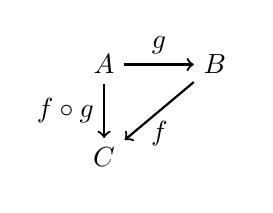
\begin{tikzpicture}[every node/.style={midway}] \matrix[column sep={4em,between origins},         row sep={2em}] at (0,0) { \node(A)   {$A$}  ; & \node(B) {$B$}; \\   \node(C) {$C$};                   \\}; \draw[<-,thick] (C) -- (A) node[anchor=east]  {$f\circ g$}; \draw[->,thick] (B) -- (C) node[anchor=north]  {$f$}; \draw[->,thick] (A)   -- (B) node[anchor=south] {$g$}; \end{tikzpicture}\end{center}

\begin{ejemplo}

Sean $A=\left\{ 1,2,3,4,5\right\} ,\:B=\left\{ 1,2,3\right\} $, $C=\left\{ 1,4,5,8\right\} $
y las funciones $g=\left\{ \left(1,2\right),\left(3,2\right),\left(4,1\right),\left(2,1\right)\right\} ,$ 

$f=\left\{ \left(2,1\right),\left(1,4\right),\left(3,5\right)\right\} $.
Determine $f\circ g$

\end{ejemplo}

\solu Note que $\left(1,2\right)\in g$ y $\left(2,1\right)\in f$,
entonces $\left(1,1\right)\in f\circ g$ de manera análoga se encuentran
todos los elementos del conjunto $f\circ g=\left\{ \left(1,1\right),\left(3,1\right),\left(4,4\right),\left(2,4\right)\right\} $,
¿será $f\circ g$ función?, se podrá asegurar de acuerdo con este
ejemplo que dada dos funciones, la composición entre ellas existe
y es función. 

\vspace*{-70pt}\begin{questionbox} 

Si suponemos que $\begin{array}{ccccc}
g & : & A & \rightarrow & B\end{array}$ y $\begin{array}{ccccc}
f & : & C & \rightarrow & D.\end{array}$ ¿ Que condición hay que pedirle a $f$ y $g$ para poder hacer la
composición $f\circ g$?

\end{questionbox} 

\resp  Si queremos definir $\left(f\circ g\right)\left(a\right)=f\left[g\left(a\right)\right]$,
entonces precisamos que $g\left(a\right)\in C$. Luego la condición
necesaria y suficiente para poder componer $f$ con $g$ es que $\mbox{Im\ensuremath{\left(f\right)\subset C,}}$
o sea que la imagen de $g$ está contenida en el dominio de $f$ . 

\subsection{\label{subsec:Operaciones-entre-proposiciones}Operaciones entre
proposiciones}

En en sistema axiomático son importantes las operaciones que se pueden
realizar con sus elementos, pero en este punto es necesario definir
lo que es una operación.

\begin{defi}{Operación binaria}{} Dados tres conjuntos $A,B$ y
$C$ no vacíos, una operación binaria es una aplicación de la forma
:

\begin{center}%
\begin{tabular}{cccc}
$\otimes$: &
$A\times B$ &
$\rightarrow$ &
\selectlanguage{english}%
$C$\selectlanguage{spanish}%
\tabularnewline
 &
$\left(x,y\right)$ &
$\mapsto$ &
$z$\tabularnewline
\end{tabular}\end{center}\vspace{-5pt}\end{defi}

\notacion Si $\left(\left(x,y\right),z\right)\in\otimes$ se denota
$x\otimes y=z.$

Note que si tenemos las aplicaciones $\begin{array}{ccccc}
g & : & A & \rightarrow & B\end{array}$, $\begin{array}{ccccc}
f & : & B & \rightarrow & C.\end{array}$ y $\begin{array}{ccccc}
h & : & A & \rightarrow & C\end{array}$ la composición de aplicaciones es una operación binaria de $\left\{ \begin{array}{ccccc}
g & : & A & \rightarrow & B\end{array}\right\} \times\left\{ \begin{array}{ccccc}
f & : & B & \rightarrow & C\end{array}\right\} \rightarrow\left\{ \begin{array}{ccccc}
h & : & A & \rightarrow & C\end{array}\right\} $ .

Como ejemplos de operaciones veremos a continuación las operaciones
entre proposiciones.

Si convenimos en considerar el conjunto $U$ de todas las posibles
proposiciones del lenguaje como conjunto universo, y además el conjunto
$V=\{v,f\}$ el conjunto de los valores de verdad de una proposición.
Entonces podemos definir las siguientes aplicaciones :

\begin{center} %
\begin{tabular}{cccc}
$P$: &
$U$ &
$\rightarrow$ &
$V$\tabularnewline
 &
$p$ &
$\mapsto$ &
$x$\tabularnewline
\end{tabular}, %
\begin{tabular}{cccc}
$\otimes$ : &
$V\times V$ &
$\rightarrow$ &
\selectlanguage{english}%
$V$\selectlanguage{spanish}%
\tabularnewline
 &
$\left(x,y\right)$ &
$\mapsto$ &
$z$\tabularnewline
\end{tabular}, %
\begin{tabular}{cccc}
$R_{\otimes}$ : &
$U\times U$ &
$\rightarrow$ &
\selectlanguage{english}%
$U$\selectlanguage{spanish}%
\tabularnewline
 &
$\left(p,q\right)$ &
$\mapsto$ &
$r$\tabularnewline
\end{tabular}y %
\begin{tabular}{cccc}
$O_{\otimes}$ : &
$U\times U$ &
$\rightarrow$ &
\selectlanguage{english}%
$V\times V$\selectlanguage{spanish}%
\tabularnewline
 &
$\left(p,q\right)$ &
$\mapsto$ &
$(x,y)$\tabularnewline
\end{tabular}\end{center}

\begin{lista}

\item La aplicación $P$ establece que a cada proposición se le puede
asignar un valor y sólo un valor de verdad, lo que está de acuerdo
con la definición, y que cada proposición tiene asignado un valor
de verdad.

\item La operación $\otimes$ establece que dados dos valores de
verdad estos se pueden operar y obtener un único valor de verdad

\item La operación $R_{\otimes}$ establece que dadas dos proposiciones
se pueden operar y obtener una única proposición.

\item La operación $O_{\otimes}$ establece que dadas dos proposiciones
se pueden operar y obtener una pareja ordenada de valores de verdad.

\end{lista}

Teniendo en cuenta las aplicaciones definidas podemos establecer las
siguientes estructuras 

\begin{center} 
\begin{large} 
\begin{tikzcd}[row sep=2cm,column sep=2cm,inner sep=1ex] 
U\times U \arrow[thick,green!40!black]{dr}[green!40!black]{\times}
\arrow[thick,red]{r}[thick,red]{R_\otimes}
\arrow[thick,blue]{d}[swap]{O_\otimes} & U \arrow[thick,red]{d}{P} \\ 
   V\times V \arrow[thick,blue]{r}[swap]{\otimes} &V 
\\   
\end{tikzcd} 
 \end{large}  
\end{center} 

En el diagrama anterior se nos muestra dos caminos para realizar la
composición $\times$ que necesitamos, el camino que se muestra en
rojo nos presenta la dificultad que sería una composición entre una
operación binaria y una aplicación, mientras que el camino que está
en azul nos muestra la composición de dos operaciones binarias por
lo que escogeremos está para construir las operaciones entre proposiciones
lógicas.

De acuerdo con lo anterior nos queda la siguiente estructura para
la operación $\times$.

\begin{center} $\times\,:\,U\times U\overset{R_{\otimes}}{\rightarrow}V\times V\overset{O_{\otimes}}{\rightarrow}V$
\end{center}

Usando ésta estructura podemos definir las siguientes operaciones
entre proposiciones.

\obs En este curso no demostraremos que las operaciones están bien
definidas, es decir que es una función y el conjunto de partida es
igual al conjunto de llegada, como tampoco la existencia y unicidad
de ellas.

\subsubsection{Conjunción}

La conjunción es la operación de la forma %
\begin{tabular}{cccc}
$O_{\wedge}$ : &
$U\times U$ &
$\rightarrow$ &
\selectlanguage{english}%
$U$\selectlanguage{spanish}%
\tabularnewline
 &
$\left(p,q\right)$ &
$\mapsto$ &
$p\wedge q$\tabularnewline
\end{tabular}de tal forma que se pueden operar sus valores de verdad usando la
definición %
\begin{tabular}{cccc}
\oper{\ensuremath{\wedge}}\,: &
$V\times V$ &
$\rightarrow$ &
\selectlanguage{english}%
$V$\selectlanguage{spanish}%
\tabularnewline
 &
$\left(x,y\right)$ &
$\mapsto$ &
$z$\tabularnewline
\end{tabular}, obtenemos una estructura de la forma: $\wedge:\:U\times U\overset{O_{\wedge}}{\rightarrow}V\times V\overset{\oper{\ensuremath{\wedge}}\,}{\rightarrow}V$.

\begin{defi}{ Conjunción}{} La ley que establece la conjunción es
la siguiente: la conjunción es verdadera, sólo si las dos proposiciones
son verdaderas.\end{defi} 
\begin{table}[H]
\centering

\caption{Tabla de verdad de la conjunción}

\setlength\arrayrulewidth{1pt}\arrayrulecolor{ptctitle} 

\begin{tabular}{c|c|c}
\arrayrulecolor{ptctitle}\hline\cellcolor{ptctitle!50}$p$ &
\cellcolor{ptctitle!50}$q$ &
\cellcolor{ptctitle!50}$p\wedge q$\tabularnewline
\hline\cellcolor{ptcbackground}$v$ &
\cellcolor{ptcbackground} $v$ &
\cellcolor{ptcbackground}$v$\tabularnewline
\hline\cellcolor{gray!50}$v$ &
\cellcolor{gray!50} $f$ &
\cellcolor{gray!50}$f$\tabularnewline
\hline\cellcolor{ptcbackground}$f$ &
\cellcolor{ptcbackground} $v$ &
\cellcolor{ptcbackground}$f$\tabularnewline
\hline\cellcolor{gray!50}$f$ &
\cellcolor{gray!50} $f$ &
\cellcolor{gray!50}$f$\tabularnewline
\end{tabular}
\end{table}

\begin{ejemplo}{\bf Conjunción}:

Sí $p:\:4<7$ y $q:\ 6\,\mbox{ es número par}$. Calcular el valor
de verdad de $p\wedge q.$ \end{ejemplo}

\solu 
\begin{table}[H]
\centering

\caption{Tabla de verdad}

\begin{tabular}{c|c|c}
\arrayrulecolor{ptctitle}\cellcolor{gray!50}$p$ &
\cellcolor{gray!50}$q$ &
\cellcolor{gray!50}$p\wedge q$\tabularnewline
\hline 
\cellcolor{ptcbackground}$v$ &
\cellcolor{ptcbackground}$v$ &
\cellcolor{ptcbackground}$v$\tabularnewline
\hline 
\end{tabular}
\end{table}


\subsubsection{Disyunción}

La disyunción es la operación de la forma %
\begin{tabular}{cccc}
$O_{\vee}$ : &
$U\times U$ &
$\rightarrow$ &
\selectlanguage{english}%
$U$\selectlanguage{spanish}%
\tabularnewline
 &
$\left(p,q\right)$ &
$\mapsto$ &
$p\vee q$\tabularnewline
\end{tabular}de tal forma que se pueden operar sus valores de verdad usando la
definición %
\begin{tabular}{cccc}
\oper{$\vee$}\,: &
$V\times V$ &
$\rightarrow$ &
\selectlanguage{english}%
$V$\selectlanguage{spanish}%
\tabularnewline
 &
$\left(x,y\right)$ &
$\mapsto$ &
$z$\tabularnewline
\end{tabular}, obtenemos una estructura de la forma: $\vee\::\,U\times U\overset{O_{\vee}}{\rightarrow}V\times V\overset{\oper{\ensuremath{\vee}}\,}{\rightarrow}V$.

\begin{defi}{ Conjunción}{} La ley que establece la disyunción es
la siguiente: la disyunción es falsa, sólo si las dos proposiciones
son falsas.\end{defi} 
\begin{table}[H]
\centering

\caption{Tabla de verdad de la disyunción}

\setlength\arrayrulewidth{1pt}\arrayrulecolor{ptctitle} 

\begin{tabular}{c|c|c}
\arrayrulecolor{ptctitle}\hline\cellcolor{ptctitle!50}$p$ &
\cellcolor{ptctitle!50}$q$ &
\cellcolor{ptctitle!50}$p\vee q$\tabularnewline
\hline\cellcolor{ptcbackground}$v$ &
\cellcolor{ptcbackground} $v$ &
\cellcolor{ptcbackground}$v$\tabularnewline
\hline\cellcolor{gray!50}$v$ &
\cellcolor{gray!50} $f$ &
\cellcolor{gray!50}$v$\tabularnewline
\hline\cellcolor{ptcbackground}$f$ &
\cellcolor{ptcbackground} $v$ &
\cellcolor{ptcbackground}$v$\tabularnewline
\hline\cellcolor{gray!50}$f$ &
\cellcolor{gray!50} $f$ &
\cellcolor{gray!50}$f$\tabularnewline
\end{tabular}
\end{table}

\begin{ejemplo}{\bf Disyunción:}
Sí $p:\:7>9$ y $q:\ 4<5$. Calcular el valor de verdad de $p\vee q.$
\end{ejemplo}

\solu 
\begin{table}[H]
\centering

\caption{Tabla de verdad}

\begin{tabular}{c|c|c}
\arrayrulecolor{ptctitle}\cellcolor{gray!50}$p$ &
\cellcolor{gray!50}$q$ &
\cellcolor{gray!50}$p\vee q$\tabularnewline
\hline 
\cellcolor{ptcbackground}$f$ &
\cellcolor{ptcbackground}$v$ &
\cellcolor{ptcbackground}$v$\tabularnewline
\hline 
\end{tabular}
\end{table}


\subsubsection{Condicional}

La condicional es la operación de la forma %
\begin{tabular}{cccc}
$O_{\rightarrow}$ : &
$U\times U$ &
$\rightarrow$ &
\selectlanguage{english}%
$U$\selectlanguage{spanish}%
\tabularnewline
 &
$\left(p,q\right)$ &
$\mapsto$ &
$p\rightarrow q$\tabularnewline
\end{tabular}de tal forma que se pueden operar sus valores de verdad usando la
definición %
\begin{tabular}{cccc}
\oper{$\rightarrow$}\,: &
$V\times V$ &
$\rightarrow$ &
\selectlanguage{english}%
$V$\selectlanguage{spanish}%
\tabularnewline
 &
$\left(x,y\right)$ &
$\mapsto$ &
$z$\tabularnewline
\end{tabular}, obtenemos una estructura de la forma: $\rightarrow\,:\,U\times U\overset{O_{\rightarrow}}{\rightarrow}V\times V\overset{\oper{\ensuremath{\rightarrow}}\,}{\rightarrow}V$.

\obs En la condicional a la proposición $p$ se le llama antecedente
y a $q$ consecuente.

\begin{defi}{ Condicional}{} La ley que establece la condicional
es la siguiente: la bicondicional es verdadera cuando las dos proposiciones
tienen el mismo valor de verdad.\end{defi}

\begin{table}[H]
\centering

\caption{Tabla de verdad de la bicondicional}

\setlength\arrayrulewidth{1pt}\arrayrulecolor{ptctitle} 

\begin{tabular}{c|c|c}
\arrayrulecolor{ptctitle}\hline\cellcolor{ptctitle!50}$p$ &
\cellcolor{ptctitle!50}$q$ &
\cellcolor{ptctitle!50}$p\longleftrightarrow q$\tabularnewline
\hline\cellcolor{ptcbackground}$v$ &
\cellcolor{ptcbackground} $v$ &
\cellcolor{ptcbackground}$v$\tabularnewline
\hline\cellcolor{gray!50}$v$ &
\cellcolor{gray!50} $f$ &
\cellcolor{gray!50}$f$\tabularnewline
\hline\cellcolor{ptcbackground}$f$ &
\cellcolor{ptcbackground} $v$ &
\cellcolor{ptcbackground}$f$\tabularnewline
\hline\cellcolor{gray!50}$f$ &
\cellcolor{gray!50} $f$ &
\cellcolor{gray!50}$v$\tabularnewline
\end{tabular}
\end{table}

\begin{ejemplo}{\bf Condicional:}

Sea $p:$ Cristóbal Colón descubrió América. ; $q:\,6+3=8$ Hallar
el valor de verdad de $p\rightarrow q$ \end{ejemplo}

\solu 
\begin{table}[H]
\centering

\caption{Tabla de verdad}

\begin{tabular}{c|c|c}
\arrayrulecolor{ptctitle}\cellcolor{gray!50}$p$ &
\cellcolor{gray!50}$q$ &
\cellcolor{gray!50}$p\leftrightarrow q$\tabularnewline
\hline 
\cellcolor{ptcbackground}$v$ &
\cellcolor{ptcbackground}$f$ &
\cellcolor{ptcbackground}$f$\tabularnewline
\hline 
\end{tabular}
\end{table}


\subsubsection{Bicondicional}

La bicondicional es la operación de la forma %
\begin{tabular}{cccc}
$O_{\longleftrightarrow}$ : &
$U\times U$ &
$\rightarrow$ &
\selectlanguage{english}%
$U$\selectlanguage{spanish}%
\tabularnewline
 &
$\left(p,q\right)$ &
$\mapsto$ &
$p\leftrightarrow q$\tabularnewline
\end{tabular}de tal forma que se pueden operar sus valores de verdad usando la
definición %
\begin{tabular}{cccc}
\oper{$\leftrightarrow$}\,: &
$V\times V$ &
$\rightarrow$ &
\selectlanguage{english}%
$V$\selectlanguage{spanish}%
\tabularnewline
 &
$\left(x,y\right)$ &
$\mapsto$ &
$z$\tabularnewline
\end{tabular}, obtenemos una estructura de la forma: $\leftrightarrow\,:\,U\times U\overset{O_{\leftrightarrow}}{\rightarrow}V\times V\overset{\oper{\ensuremath{\leftrightarrow}}\,}{\rightarrow}V$.

\begin{defi}{ Bicondicional}{} La ley que establece la bicondicional
es la siguiente: la bicondicional es verdadera cuando las dos proposiciones
tienen el mismo valor de verdad.\end{defi}

\begin{table}[H]
\centering

\caption{Tabla de verdad de la bicondicional}

\setlength\arrayrulewidth{1pt}\arrayrulecolor{ptctitle} 

\begin{tabular}{c|c|c}
\arrayrulecolor{ptctitle}\hline\cellcolor{ptctitle!50}$p$ &
\cellcolor{ptctitle!50}$q$ &
\cellcolor{ptctitle!50}$p\longleftrightarrow q$\tabularnewline
\hline\cellcolor{ptcbackground}$v$ &
\cellcolor{ptcbackground} $v$ &
\cellcolor{ptcbackground}$v$\tabularnewline
\hline\cellcolor{gray!50}$v$ &
\cellcolor{gray!50} $f$ &
\cellcolor{gray!50}$f$\tabularnewline
\hline\cellcolor{ptcbackground}$f$ &
\cellcolor{ptcbackground} $v$ &
\cellcolor{ptcbackground}$f$\tabularnewline
\hline\cellcolor{gray!50}$f$ &
\cellcolor{gray!50} $f$ &
\cellcolor{gray!50}$v$\tabularnewline
\end{tabular}
\end{table}

\begin{ejemplo}{\bf Bicondicional:}

Sea $p:$ Cristóbal Colón descubrió América. ; $q:\,6+3=8$ Hallar
el valor de verdad de $p\rightarrow q$ \end{ejemplo}

\solu

\begin{table}[H]
\centering

\caption{Tabla de verdad}

\begin{tabular}{c|c|c}
\arrayrulecolor{ptctitle}\cellcolor{gray!50}$p$ &
\cellcolor{gray!50}$q$ &
\cellcolor{gray!50}$p\rightarrow q$\tabularnewline
\hline 
\cellcolor{ptcbackground}$v$ &
\cellcolor{ptcbackground}$f$ &
\cellcolor{ptcbackground}$f$\tabularnewline
\hline 
\end{tabular}
\end{table}


\subsubsection{Disyunción exclusiva}

La disyunción exclusiva es la operación de la forma %
\begin{tabular}{cccc}
$O_{\veebar}$ : &
$U\times U$ &
$\rightarrow$ &
\selectlanguage{english}%
$U$\selectlanguage{spanish}%
\tabularnewline
 &
$\left(p,q\right)$ &
$\mapsto$ &
$p\veebar q$\tabularnewline
\end{tabular}de tal forma que se pueden operar sus valores de verdad usando la
definición %
\begin{tabular}{cccc}
\oper{$\veebar$}\,: &
$V\times V$ &
$\rightarrow$ &
\selectlanguage{english}%
$V$\selectlanguage{spanish}%
\tabularnewline
 &
$\left(x,y\right)$ &
$\mapsto$ &
$z$\tabularnewline
\end{tabular}, obtenemos una estructura de la forma: $\veebar\,:\,U\times U\overset{O_{\veebar}}{\rightarrow}V\times V\overset{\oper{\ensuremath{\veebar}}\,}{\rightarrow}V$.

\begin{defi}{ Disyunción exclusiva}{} La ley que establece la disyunción
exclusiva es la siguiente: la disyunción exclusiva es falsa cuando
las dos proposiciones tienen el mismo valor de verdad.\end{defi}

\begin{table}[H]
\centering

\caption{Tabla de verdad de la bicondicional}

\setlength\arrayrulewidth{1pt}\arrayrulecolor{ptctitle} 

\begin{tabular}{c|c|c}
\arrayrulecolor{ptctitle}\hline\cellcolor{ptctitle!50}$p$ &
\cellcolor{ptctitle!50}$q$ &
\cellcolor{ptctitle!50}$p\veebar q$\tabularnewline
\hline\cellcolor{ptcbackground}$v$ &
\cellcolor{ptcbackground} $v$ &
\cellcolor{ptcbackground}$f$\tabularnewline
\hline\cellcolor{gray!50}$v$ &
\cellcolor{gray!50} $f$ &
\cellcolor{gray!50}$v$\tabularnewline
\hline\cellcolor{ptcbackground}$f$ &
\cellcolor{ptcbackground} $v$ &
\cellcolor{ptcbackground}$v$\tabularnewline
\hline\cellcolor{gray!50}$f$ &
\cellcolor{gray!50} $f$ &
\cellcolor{gray!50}$f$\tabularnewline
\end{tabular}
\end{table}

\begin{ejemplo}{\bf Disyunción exclusiva:}

Sea $p:$ Cristóbal Colón descubrió América. ; $q:\,6+3=8$ Hallar
el valor de verdad de $p\veebar q$ \end{ejemplo}

\obs Ésta operación se llama excluyente porque porque sólo se puede
dar ambas pero no una sola. 

\solu

\begin{table}[H]
\centering

\caption{Tabla de verdad}

\begin{tabular}{c|c|c}
\arrayrulecolor{ptctitle}\cellcolor{gray!50}$p$ &
\cellcolor{gray!50}$q$ &
\cellcolor{gray!50}$p\veebar q$\tabularnewline
\hline 
\cellcolor{ptcbackground}$v$ &
\cellcolor{ptcbackground}$f$ &
\cellcolor{ptcbackground}$v$\tabularnewline
\hline 
\end{tabular}
\end{table}


\subsubsection{Negación}

Para la negación usamos las operaciones de la forma %
\begin{tabular}{cccc}
$P$ : &
$U$ &
$\rightarrow$ &
\selectlanguage{english}%
$V$\selectlanguage{spanish}%
\tabularnewline
 &
$p$ &
$\mapsto$ &
$x$\tabularnewline
\end{tabular}y %
\begin{tabular}{cccc}
$P_{\sim}$ : &
$V$ &
$\rightarrow$ &
\selectlanguage{english}%
$V$\selectlanguage{spanish}%
\tabularnewline
 &
$x$ &
$\mapsto$ &
$y$\tabularnewline
\end{tabular}tal que $x\neq y$. para construir la composición $\sim:\;U\overset{P}{\rightarrow}V\overset{P_{\sim}}{\rightarrow}V$

\begin{defi}{Negación}{} La ley que establece la negación es la
siguiente: La negación cambia el valor de verdad de una proposición.\end{defi}

Su tabla de verdad es la siguiente

\begin{table}[H]
\centering

\caption{Tabla de verdad de la negación.}

\begin{tabular}{c|c}
\arrayrulecolor{ptctitle}\cellcolor{ptctitle!50}$p$ &
\cellcolor{ptctitle!50}$\sim p$\tabularnewline
\hline 
\cellcolor{ptcbackground}$v$ &
\cellcolor{ptcbackground}$f$\tabularnewline
\hline 
\cellcolor{gray!50}$f$ &
\cellcolor{gray!50} $v$\tabularnewline
\end{tabular}
\end{table}


\subsection{\label{subsec:Relaciones-entre-proposiciones}Relaciones entre proposiciones}

En esta sección trabajaremos con tautologías y falacias por lo que
presentaremos algunos ejemplos para aprender a determinar cuando una
proposición es una tautología, contingencia ó falacia.

\begin{ejemplo}{\bf Tautológias:}
\begin{enumerate}
\item $p\vee\sim p$ (principio del tercio excluido) 
\item $\left[(p\rightarrow q)\wedge p\right]\rightarrow q$
\item $\sim\left(p\wedge\sim p\right)$
\end{enumerate}
\end{ejemplo}

\solu
\begin{enumerate}
\item Vemos que en la última columna de la tabla de verdad (\ref{tau1})
nos muestra que $p\vee\sim p$ es una tautología. 
\begin{table}[H]
\centering

\caption{Tabla de verdad.}
\label{tau1}

\begin{tabular}{c|c|c}
\arrayrulecolor{ptctitle}\cellcolor{ptctitle!50}$p$ &
\cellcolor{ptctitle!50}$\sim p$ &
\cellcolor{ptctitle!50}$p\vee\sim p$\tabularnewline
\hline 
\cellcolor{ptcbackground} $v$ &
\cellcolor{ptcbackground}$f$ &
\cellcolor{ptcbackground}$v$\tabularnewline
\hline 
\cellcolor{gray!50}$f$ &
\cellcolor{gray!50} $v$ &
\cellcolor{gray!50}$v$\tabularnewline
\hline 
\end{tabular}
\end{table}
\item Si observamos en la tabla de verdad (\ref{tau2}) nos queda demostrado
que $\left[(p\rightarrow q)\wedge p\right]\rightarrow q$ es una tautología.
\begin{table}[H]
\centering

\caption{Tabla de verdad.}
\label{tau2}

\begin{tabular}{c|c|c|c|c}
\arrayrulecolor{ptctitle}\cellcolor{ptctitle!50}$p$ &
\cellcolor{ptctitle!50}$q$ &
\cellcolor{ptctitle!50}$p\rightarrow q$ &
\cellcolor{ptctitle!50}$\left(p\rightarrow q\right)\wedge p$ &
\cellcolor{ptctitle!50}$\left[\left(p\rightarrow p\right)\wedge p\right]\rightarrow q$\tabularnewline
\hline 
\cellcolor{ptcbackground} $v$ &
\cellcolor{ptcbackground}$v$ &
\cellcolor{ptcbackground}$v$ &
\cellcolor{ptcbackground}$v$ &
\cellcolor{ptcbackground}$v$\tabularnewline
\hline 
\cellcolor{gray!50}$v$ &
\cellcolor{gray!50} $f$ &
\cellcolor{gray!50}$f$ &
\cellcolor{gray!50}$f$ &
\cellcolor{gray!50}$v$\tabularnewline
\hline 
\cellcolor{ptcbackground}$f$ &
\cellcolor{ptcbackground} $v$ &
\cellcolor{ptcbackground} $v$ &
\cellcolor{ptcbackground}$f$ &
\cellcolor{ptcbackground}$v$\tabularnewline
\hline 
\cellcolor{gray!50} $f$ &
\cellcolor{gray!50} $f$ &
\cellcolor{gray!50} $v$ &
\cellcolor{gray!50}$f$ &
\cellcolor{gray!50}$v$\tabularnewline
\hline 
\end{tabular}
\end{table}
\item Este queda de ejercicio al lector.
\end{enumerate}
\begin{ejemplo}{\bf Falacias:}
\begin{enumerate}
\item $p\wedge\sim p$ (principio de contradicción) 
\item $(p\rightarrow q)\wedge\left(p\wedge\sim q\right)$
\item $\sim\left(p\vee\sim p\right)$
\end{enumerate}
\end{ejemplo}

\solu
\begin{enumerate}
\item Vemos que en la última columna de la tabla de verdad (\ref{fal1})
nos muestra que $p\wedge\sim p$ es una falacia. 
\begin{table}[H]
\centering

\caption{Tabla de verdad.}
\label{fal1}

\begin{tabular}{c|c|c}
\arrayrulecolor{ptctitle}\cellcolor{ptctitle!50}$p$ &
\cellcolor{ptctitle!50}$\sim p$ &
\cellcolor{ptctitle!50}$p\wedge\sim p$\tabularnewline
\hline 
\cellcolor{ptcbackground} $v$ &
\cellcolor{ptcbackground}$f$ &
\cellcolor{ptcbackground}$f$\tabularnewline
\hline 
\cellcolor{gray!50}$f$ &
\cellcolor{gray!50} $v$ &
\cellcolor{gray!50}$f$\tabularnewline
\hline 
\end{tabular}
\end{table}
\item Si observamos en la tabla de verdad (\ref{fal2}) nos queda demostrado
que $(p\rightarrow q)\wedge\left(p\wedge\sim q\right)$ es una falacia.
\begin{table}[H]
\centering

\caption{Tabla de verdad.}
\label{fal2}

\begin{tabular}{c|c|c|c|c}
\arrayrulecolor{ptctitle}\cellcolor{ptctitle!50}$p$ &
\cellcolor{ptctitle!50}$q$ &
\cellcolor{ptctitle!50}$p\rightarrow q$ &
\cellcolor{ptctitle!50}$p\wedge\sim q$ &
\cellcolor{ptctitle!50}$(p\rightarrow q)\wedge\left(p\wedge\sim q\right)$\tabularnewline
\hline 
\cellcolor{ptcbackground} $v$ &
\cellcolor{ptcbackground}$v$ &
\cellcolor{ptcbackground}$v$ &
\cellcolor{ptcbackground}$f$ &
\cellcolor{ptcbackground}$f$\tabularnewline
\hline 
\cellcolor{gray!50}$v$ &
\cellcolor{gray!50} $f$ &
\cellcolor{gray!50}$f$ &
\cellcolor{gray!50}$v$ &
\cellcolor{gray!50}$f$\tabularnewline
\hline 
\cellcolor{ptcbackground}$f$ &
\cellcolor{ptcbackground} $v$ &
\cellcolor{ptcbackground} $v$ &
\cellcolor{ptcbackground}$f$ &
\cellcolor{ptcbackground}$f$\tabularnewline
\hline 
\cellcolor{gray!50} $f$ &
\cellcolor{gray!50} $f$ &
\cellcolor{gray!50} $v$ &
\cellcolor{gray!50}$f$ &
\cellcolor{gray!50}$f$\tabularnewline
\hline 
\end{tabular}
\end{table}
\item Este queda de ejercicio al lector
\end{enumerate}

\subsubsection{Implicación}

\begin{defi}{Implicación}{} Se dice que una proposición $q$ se
deduce de $p$ o que una proposición $p$ implica una proposición
$q$ cuando $p\rightarrow q$ es una tautología.\end{defi}

\notacion  Si una proposición $p$ implica a una proposición $q$
se denota $p\Rightarrow q$ o $p\,\triangleright:\,q$ que se lee
$q$ se deduce de $p$, también se puede leer si tenemos $p$ se deduce
$q.$

\obs El hecho que $p$ implique $q$ quiere decir que se puede obtener
$q$ a partir de de $p$ o que si $p$ es verdadera $q$ también lo
es.

\begin{ejemplo}{\bf Implicación:}

Determinar si $\left[\left(\sim p\vee q\right)\wedge\sim q\right]\Rightarrow\sim p$
\end{ejemplo}

\solu 
\begin{table}[H]
\centering

\caption{Tabla de verdad.}

\begin{tabular}{c|c|c|c|c|c|c}
\arrayrulecolor{ptctitle}\cellcolor{ptctitle!50}$p$ &
\cellcolor{ptctitle!50}$q$ &
\cellcolor{ptctitle!50}$\sim p$ &
\cellcolor{ptctitle!50}$\sim p\vee q$ &
\cellcolor{ptctitle!50}$\sim q$ &
\cellcolor{ptctitle!50}\foreignlanguage{english}{$\left(\sim p\vee q\right)\wedge\sim q$} &
\cellcolor{ptctitle!50}$\left[\left(\sim p\vee q\right)\wedge\sim q\right]\rightarrow\sim p$ \tabularnewline
\hline 
\cellcolor{ptcbackground} $v$ &
\cellcolor{ptcbackground}$v$ &
\cellcolor{ptcbackground}$f$ &
\cellcolor{ptcbackground}$f$ &
\cellcolor{ptcbackground}$v$ &
\cellcolor{ptcbackground}$v$ &
\cellcolor{ptcbackground}$v$\tabularnewline
\hline 
\cellcolor{gray!50}$v$ &
\cellcolor{gray!50} $f$ &
\cellcolor{gray!50}$f$ &
\cellcolor{gray!50}$f$ &
\cellcolor{gray!50}$v$ &
\cellcolor{gray!50}$f$ &
\cellcolor{gray!50}$v$\tabularnewline
\hline 
\cellcolor{ptcbackground}$f$ &
\cellcolor{ptcbackground} $v$ &
\cellcolor{ptcbackground} $v$ &
\cellcolor{ptcbackground}$f$ &
\cellcolor{ptcbackground}$v$ &
\cellcolor{ptcbackground}$v$ &
\cellcolor{ptcbackground}$v$\tabularnewline
\hline 
\cellcolor{gray!50} $f$ &
\cellcolor{gray!50} $f$ &
\cellcolor{gray!50} $v$ &
\cellcolor{gray!50}$f$ &
\cellcolor{gray!50}$v$ &
\cellcolor{gray!50}$v$ &
\cellcolor{gray!50}$v$\tabularnewline
\hline 
\end{tabular}
\end{table}

\begin{ejemplo}{\bf Implicación:}

Determinar si $\left(p\wedge\sim p\right)\Rightarrow q$ \end{ejemplo}

\solu 
\begin{table}[H]
\centering

\caption{Tabla de verdad.}

\begin{tabular}{c|c|c|c|c}
\arrayrulecolor{ptctitle}\cellcolor{ptctitle!50}$p$ &
\cellcolor{ptctitle!50}$q$ &
\cellcolor{ptctitle!50}$\sim p$ &
\cellcolor{ptctitle!50}$p\wedge\sim p$ &
\cellcolor{ptctitle!50}$\left(p\wedge\sim p\right)\rightarrow q$\tabularnewline
\hline 
\cellcolor{ptcbackground} $v$ &
\cellcolor{ptcbackground}$v$ &
\cellcolor{ptcbackground}$f$ &
\cellcolor{ptcbackground}$f$ &
\cellcolor{ptcbackground}$v$\tabularnewline
\hline 
\cellcolor{gray!50}$v$ &
\cellcolor{gray!50} $f$ &
\cellcolor{gray!50}$f$ &
\cellcolor{gray!50}$f$ &
\cellcolor{gray!50}$v$\tabularnewline
\hline 
\cellcolor{ptcbackground}$f$ &
\cellcolor{ptcbackground} $v$ &
\cellcolor{ptcbackground} $v$ &
\cellcolor{ptcbackground}$f$ &
\cellcolor{ptcbackground}$v$\tabularnewline
\hline 
\cellcolor{gray!50} $f$ &
\cellcolor{gray!50} $f$ &
\cellcolor{gray!50} $v$ &
\cellcolor{gray!50}$f$ &
\cellcolor{gray!50}$v$\tabularnewline
\hline 
\end{tabular}
\end{table}

Cuando verificamos que $p\Rightarrow q$ en realidad estamos comparando
el conjunto solución de $p$ y el conjunto solución de $q.$ Desde
ese punto de vista $p\Rightarrow q$ si y solo si el conjunto solución
de $p$ es subconjunto del conjunto solución de $q.$

\subsubsection{Equivalencia lógica}

\begin{defi}{Equivalencia lógica}{} Se dice que una proposición
$q$ es equivalente a $p$, cuando $p\leftrightarrow q$ es una tautología.\end{defi}

\notacion  Si una proposición $p$ es equivalente a una proposición
$q$ se denota $p\Leftrightarrow q$ ó $p\equiv q.$

\obs Que $p\equiv q$ quiere decir que se puede intercambiar $p$
y $q$ sin afectar el valor de verdad de la proposición. También expresa
que los conjuntos soluciones de $p$ y $q$ son iguales y eso se verifica
al observar que si $p\equiv q$, $p$ y $q$ tiene la misma tabla
de verdad.

\begin{ejemplo}{\bf Equivalencia lógica:}

Analice el valor de verdad de la proposición compuesta \ensuremath{(p\rightarrow q)\leftrightarrow(\sim q\rightarrow\sim p)}
\end{ejemplo}

\solu

\selectlanguage{english}%
\begin{tabular}{ccccccc} \ensuremath{p} &  \ensuremath{q} &  \ensuremath{p\rightarrow q} &  \ensuremath{\sim q} &  \ensuremath{\sim p} &  \ensuremath{\sim q\rightarrow\sim p} &  \ensuremath{(p\rightarrow q)\leftrightarrow(\sim q\rightarrow\sim p)}\\V  &  V  &  V  &  F  &  F  &  V  &  V\\V  &  F  &  F  &  V  &  F  &  F  &  V\\F  &  V  &  V  &  F  &  V  &  V  &  V\\F  &  F  &  V  &  V  &  V  &  V  &  V \end{tabular}\ 

\selectlanguage{spanish}%
Es decir las proposiciones: $p\rightarrow q$ y $\sim q\rightarrow\sim p$\ son
equivalentes.

\begin{ejemplo}{\bf Equivalencia lógica:}

Probar usando las tablas de verdad que las proposiciones $(p\rightarrow q)$
y $(\sim q\rightarrow\sim p)$, son lógicamente equivalentes. 

\end{ejemplo}

\solu Para probar que las proposiciones $(p\rightarrow q)$ y $(\sim q\rightarrow\sim p)$
son lógicamente equivalentes debemos probar que $(p\rightarrow q)$
$\leftrightarrow$ $(\sim q\rightarrow\sim p)$ es una tautología.
\begin{table}[H]
\centering

\caption{Tabla de verdad.}
\label{equil1}

\begin{tabular}{c|c|c|c|c|c|c}
\arrayrulecolor{ptctitle}\cellcolor{ptctitle!50}$p$ &
\cellcolor{ptctitle!50}$q$ &
\cellcolor{ptctitle!50}$\sim p$ &
\cellcolor{ptctitle!50}$\sim q$ &
\cellcolor{ptctitle!50}$p\rightarrow q$ &
\cellcolor{ptctitle!50}\foreignlanguage{english}{$\sim q\rightarrow\sim p$} &
\cellcolor{ptctitle!50}$(p\rightarrow q)$ $\leftrightarrow$ $(\sim q\rightarrow\sim p)$\tabularnewline
\hline 
\cellcolor{ptcbackground} $v$ &
\cellcolor{ptcbackground}$v$ &
\cellcolor{ptcbackground}$f$ &
\cellcolor{ptcbackground}$f$ &
\cellcolor{ptcbackground}$v$ &
\cellcolor{ptcbackground}$v$ &
\cellcolor{ptcbackground}$v$\tabularnewline
\hline 
\cellcolor{gray!50}$v$ &
\cellcolor{gray!50} $f$ &
\cellcolor{gray!50}$f$ &
\cellcolor{gray!50}$v$ &
\cellcolor{gray!50}$f$ &
\cellcolor{gray!50}$f$ &
\cellcolor{gray!50}$v$\tabularnewline
\hline 
\cellcolor{ptcbackground}$f$ &
\cellcolor{ptcbackground} $v$ &
\cellcolor{ptcbackground} $v$ &
\cellcolor{ptcbackground}$f$ &
\cellcolor{ptcbackground}$v$ &
\cellcolor{ptcbackground}$v$ &
\cellcolor{ptcbackground}$v$\tabularnewline
\hline 
\cellcolor{gray!50} $f$ &
\cellcolor{gray!50} $f$ &
\cellcolor{gray!50} $v$ &
\cellcolor{gray!50}$v$ &
\cellcolor{gray!50}$v$ &
\cellcolor{gray!50}$v$ &
\cellcolor{gray!50}$v$\tabularnewline
\hline 
\end{tabular}
\end{table}

\obs Para verificar si dos proposiciones son lógicamente equivalentes
basta comprobar que las dos proposiciones tienen la misma tabla de
verdad. Como se observa en la tabla (\ref{equil1}) al comparar las
columnas $5$ y $6$.

\section{Inferencia y esquemas de razonamiento}

\subsection{Principales leyes lógicas o tautológicas}

Siguiendo las construcción axiomática de la lógica nos queda establecer
los axiomas y los teoremas, cual estableceremos en ésta sección. 

\begin{ideabox}{\bf Leyes de inferencia lógica:}

Dadas dos proposiciones $p$ y $q$ al término $p\equiv q$ se le
llama ley de inferencia.

\end{ideabox}

En la lógica los teoremas son leyes de inferencia.

\subsubsection{Axiomas}

Estableceremos tres axiomas,

\begin{axioma}{ Identidad}{}Toda proposición es idéntica a si misma,
es decir $p\equiv p$\end{axioma}

\begin{axioma}{Contradicción }{}Una proposición no puede ser cierta
y falsa a la vez, es decir $\sim\left(p\wedge\sim p\right)\equiv v.$\end{axioma}

\begin{axioma}{Tercer excluido }{}Toda proposición es cierta ó es
falsa , es decir $p\vee\sim p\equiv v.$\end{axioma}

\subsubsection{Leyes de inferencia básicas.}

Trataremos de presentar las leyes de inferencia que se deben demostrar
utilizando tablas de verdad. (no son un conjunto mínimo de leyes de
inferencias básicas)

\begin{ley}{Involutiva}

$\sim\left(\sim p\right)\equiv p$

\end{ley}

\begin{ley}{Indempotencia}
\begin{enumerate}
\item $p\wedge p\equiv p$
\item $p\vee p\equiv p$
\end{enumerate}
\end{ley}

\begin{ley}{falsos modulos o de la adición}
\begin{enumerate}
\item $p\wedge f\equiv f$
\item $p\vee v\equiv v$
\end{enumerate}
\end{ley}

\begin{ley}{Comutativas}
\begin{enumerate}
\item $\left(p\wedge q\right)\equiv\left(q\wedge p\right)$
\item $\left(p\vee q\right)\equiv\left(q\vee p\right)$
\item $p\leftrightarrow q\equiv q\leftrightarrow p$
\end{enumerate}
\end{ley}

\begin{ley}{Asociativas}
\begin{enumerate}
\item $p\wedge\left(q\wedge r\right)\equiv\left(p\wedge q\right)\wedge r$
\item $p\vee\left(q\vee r\right)\equiv\left(p\vee q\right)\vee r$
\item $p\leftrightarrow\left(q\leftrightarrow r\right)\equiv\left(p\leftrightarrow q\right)\leftrightarrow r$
\end{enumerate}
\end{ley}

\begin{ley}{Distributivas}
\begin{enumerate}
\item $p\wedge\left(q\vee r\right)\equiv\left(p\wedge q\right)\vee\left(p\wedge r\right)$
\item $p\vee\left(q\wedge r\right)\equiv\left(p\vee q\right)\wedge\left(p\vee r\right)$
\item $p\rightarrow\left(q\vee r\right)\equiv\left(p\rightarrow q\right)\vee\left(p\rightarrow r\right)$
\item $p\rightarrow\left(q\wedge r\right)\equiv\left(p\rightarrow q\right)\wedge\left(p\rightarrow r\right)$
\end{enumerate}
\end{ley}

\begin{ley}{Morgan}
\begin{enumerate}
\item $\sim\left(p\wedge q\right)\equiv\sim p\text{\,}\vee\sim q$
\item $\sim\left(p\vee q\right)\equiv\sim p\,\wedge\sim q$
\end{enumerate}
\end{ley}

\begin{ley}{Del condicional}
\begin{enumerate}
\item $p\rightarrow q\equiv\sim p\vee q$
\item $\sim\left(p\rightarrow q\right)\equiv p\,\wedge\sim q$
\end{enumerate}
\end{ley}

\begin{ley}{Del bicondicional}
\begin{enumerate}
\item $p\leftrightarrow q\equiv\left(p\rightarrow q\right)\wedge\left(q\rightarrow p\right)$
\item $p\leftrightarrow q\equiv\left(p\wedge q\right)\vee\left(\sim p\,\vee\sim q\right)$
\end{enumerate}
\end{ley}

\begin{ley}{De la absorción}
\begin{enumerate}
\item $p\wedge\left(p\text{\,\ensuremath{\vee}\ensuremath{q}}\right)\equiv p$
\item $p\wedge\left(\sim p\vee q\right)\equiv p\wedge q$
\item $p\vee\left(p\wedge q\right)\equiv p$
\item $p\vee\left(\sim p\wedge q\right)\equiv p\vee q$
\end{enumerate}
\end{ley}

\begin{ley}{De transposición}
\begin{enumerate}
\item $\left(p\rightarrow q\right)\equiv\sim q\rightarrow\sim p$ contrareciproco
\item $p\leftrightarrow q\equiv\sim q\leftrightarrow\sim p$
\end{enumerate}
\end{ley}

\begin{ley}{De exportación}
\begin{enumerate}
\item $\left(p\wedge q\right)\rightarrow r\equiv p\rightarrow\left(q\rightarrow r\right)$
\item $\left(p_{1}\wedge p_{2}\wedge p_{3}\wedge\cdots\wedge p_{n}\right)\rightarrow r\equiv\left(p_{1}\wedge p_{2}\wedge p_{3}\wedge\cdots\wedge p_{n-1}\right)\rightarrow\left(p_{n}\rightarrow r\right)$
\end{enumerate}
\end{ley}

\begin{ley}{De los modulos}
\begin{enumerate}
\item $p\wedge v\equiv p$ 
\item $p\vee f\equiv p$
\end{enumerate}
\end{ley}

\begin{ley}{De la simplificación}
\begin{enumerate}
\item $\left(p\vee q\right)\wedge\left(p\,\vee\sim q\right)\equiv p$
\item $\left(p\wedge q\right)\vee\left(p\,\wedge\sim q\right)\equiv p$
\end{enumerate}
\end{ley}

\obs Estas Leyes son muy útiles para simplificar los problemas, puesto
que es válido reemplazar una proposición por su equivalente sin alterar
el resultado. 

\begin{ejemplo}

Simplificar las proposiciones siguientes aplicando las leyes lógicas 
\begin{enumerate}
\item $\left(p\wedge q\right)\wedge\sim\left(p\wedge q\right).$
\item $\left[\left(p\vee\sim q\right)\wedge q\right]\rightarrow p$.
\item $\sim\left[\sim\left(p\wedge q\right)\rightarrow\sim q\right]\vee q.$
\item $\left[\left(\sim p\wedge q\right)\rightarrow\left(r\wedge\sim r\right)\right]\wedge\sim q.$
\item $\left[\left(p\wedge q\right)\wedge q\right]\longleftrightarrow\left[p\wedge\left(q\wedge q\right)\right].$
\item $\left(p\rightarrow q\right)\vee\left[\sim\left(p\longleftrightarrow\sim q\right)\right].$
\item $(p\rightarrow q)\leftrightarrow{(p\wedge\sim q)\rightarrow q}$
\end{enumerate}
\end{ejemplo}

\solu
\begin{enumerate}
\item Apliquemos las leyes de inferencia
\begin{eqnarray*}
\left(p\wedge q\right)\wedge\left[\sim\left(p\wedge q\right)\right] & \equiv & \left(p\wedge q\right)\wedge\underset{\mbox{morgan}}{\left[\sim p\vee\sim q\right]}\\
 & \equiv & \underset{\mbox{distributiva}}{\left[\left(p\wedge q\right)\wedge\sim p\right]\vee\left[\left(p\wedge q\right)\text{\ensuremath{\wedge\sim}\ensuremath{q}}\right]}\\
 & \equiv & \underset{\mbox{conmutativa}}{\left[\left(q\wedge p\right)\wedge\sim p\right]}\vee\underset{\mbox{asociativa}}{\left[p\wedge\left(q\wedge\sim q\right)\right]}\\
 & \equiv & \underset{\mbox{asociativa}}{\left[q\wedge\left(p\wedge\sim p\right)\right]}\vee\underset{\mbox{contadicción}}{\left[p\wedge f\right]}\\
 & \equiv & \underset{\mbox{contradicción}}{\left(q\wedge f\right)}\vee\underset{\mbox{falso modulo}}{f}\\
 & \equiv & \underset{\mbox{falso modulo}}{f}\vee f\\
 & \equiv & f
\end{eqnarray*}
\item Apliquemos las leyes de inferencia (indique las leyes aplicadas) 
\begin{eqnarray*}
\left[\left(p\vee\sim q\right)\wedge q\right]\rightarrow p & \equiv & \sim\left[\left(p\vee\sim q\right)\wedge q\right]\vee p\\
 & \equiv & \left[\sim\left(p\vee\sim q\right)\vee\sim q\right]\vee p\\
 & \equiv & \left[\sim\left(p\vee\sim q\right)\right]\vee\left(p\vee\sim q\right)\\
 & \equiv & \left(\sim\left(p\vee\sim q\right)\vee p\right)\vee\sim q\\
 & \equiv & \left(\left[\sim p\wedge\sim q\right]\vee p\right)\vee\sim q\\
 & \equiv & \left[\left(\sim p\vee p\right)\wedge\left(\sim q\vee p\right)\right]\vee\sim q\\
 & \equiv & \left[v\wedge\left(\sim q\vee p\right)\right]\vee\sim q\\
 & \equiv & \left(\sim q\vee p\right)\vee\sim q\\
 & \equiv & \left(p\vee\sim q\right)\vee\sim q\\
 & \equiv & p\vee\left(\sim q\vee\sim q\right)\\
 & \equiv & p\vee\sim q
\end{eqnarray*}
\item Apliquemos las leyes de inferencia (indique las leyes aplicadas)
\begin{eqnarray*}
\sim\left[\sim\left(p\wedge q\right)\rightarrow\sim q\right]\vee q & \equiv & \left[\sim\left(p\wedge q\right)\wedge\sim\left(\sim q\right)\right]\vee q\\
 & \equiv & \left[\left(\sim p\vee\sim q\right)\wedge q\right]\vee q\\
 & \equiv & \left[\left(\sim p\wedge q\right)\vee\left(\sim q\wedge q\right)\right]\vee q\\
 & \equiv & \left[\left(\sim p\wedge\sim q\right)\vee f\right]\vee q\\
 & \equiv & \left(\sim p\wedge\sim q\right)\vee q\\
 & \equiv & \left(\left(\sim p\vee q\right)\wedge\left(\sim q\vee q\right)\right)\\
 & \equiv & \left(\sim p\vee q\right)\wedge v\\
 & \equiv & \sim p\vee q
\end{eqnarray*}
El resto de los ejemplos quedan de ejercicio para el lector.
\end{enumerate}

\subsection{\label{subsec:Esquemas-de-razonamiento}Esquemas de razonamiento}

Las leyes de inferencia nos ayuda a construir esquemas mentales que
nos sirven para construir demostraciones, es decir cada ley de inferencia
es un esquema de razonamiento.

\subsubsection{Método inductivo}

El razonamiento inductivo es el proceso mediante el cual se obtienen
conclusiones a partir de nuestras propias observaciones o a partir
de ejemplos particulares, es decir al observar que una acción o propiedad
se repite se concluye en general que esa acción o propiedad siempre
es cierta 

\vspace*{-70pt}\begin{ideabox}{\bf Conjetura:}

Es la conclusión que se obtiene a partir de un proceso inductivo 

\end{ideabox}

Todas las proposiciones que tomamos como conjetura deben tener la
forma de una implicación o de una equivalencia, por tanto es necesario
conocer las diferentes formas de representar una implicación.

\obs Al utilizar el razonamiento inductivo debemos tener cuidado
de no construir conjeturas o generalizaciones falsas, por lo siempre
hay que tratar de encontrar casos donde no se cumpla la conjetura,
en caso de que no se consiga, no quiere decir que la conjetura es
cierta, sólo nos indica que no hemos encontrado un caso donde no se
cumple. A continuación mostraremos un ejemplo para explicar paso a
paso como podemos obtener una conjetura a partir de una secuencia
de casos o fenómenos. Aunque en ese ejemplo no trataremos de verificar
si la conjetura es siempre cierta, el objetivo es de aprender a construir
conjeturas. 

\begin{ejemplo} Suponga que una persona mide los lados de cuatro
triángulos como muestra la figura(\ref{dest}). Establezca una conjetura
sobre los lados de un triángulo

\end{ejemplo}

\begin{figure}[H]
\centering\caption{Desigualdad triangular}
\label{dest}

 \definecolor{xdxdff}{rgb}{0.49,0.49,1}
\definecolor{qqqqff}{rgb}{0,0,1}
\begin{tikzpicture}[scale=1.50, font=\fontsize{8}{9}\selectfont,line cap=round,line join=round,>=triangle 45,x=1.0cm,y=1.0cm] 
\clip(-2.49,3.16) rectangle (4.47,5.53);
\draw (-1.92,3.96)-- (-1.15,3.96); 
\draw (-1.92,3.96)-- (-1.38,4.5); 
\draw (-1.38,4.5)-- (-1.15,3.96);
\draw (0.2,4.68)-- (-0.07,3.97);
\draw (0.2,4.68)-- (0.51,3.98); 
\draw (0.51,3.98)-- (-0.07,3.97);
\draw (1.42,4.22)-- (2.03,4.22);
\draw (1.07,4.72)-- (1.42,4.22); 
\draw (1.07,4.72)-- (2.03,4.22); 
\draw (3.44,4.72)-- (3.02,4.27);
\draw (3.44,4.72)-- (3.89,4.3); 
\draw (3.89,4.3)-- (3.02,4.27);
\begin{scriptsize} 
\fill [color=qqqqff] (-1.92,3.96) circle (1.5pt);
\draw[color=qqqqff] (-2.04,3.97) node {$A$};
\fill [color=xdxdff] (-1.15,3.96) circle (1.5pt);
\draw[color=xdxdff] (-1.06,3.88) node {$B$};
\draw[color=black] (-1.56,3.84) node {$0.77$};
\fill [color=xdxdff] (-1.38,4.5) circle (1.5pt);
\draw[color=xdxdff] (-1.4,4.75) node {$C$}; 
\draw[color=black] (-1.88,4.43) node {$0.77$};
\draw[color=black] (-0.96,4.29) node {$0.59$};
\fill [color=qqqqff] (0.2,4.68) circle (1.5pt);
\draw[color=qqqqff] (0.19,4.85) node {$D$}; \fill [color=xdxdff] (-0.07,3.97) circle (1.5pt); \draw[color=xdxdff] (-0.22,3.97) node {$E$};
\draw[color=black] (-0.2,4.51) node {$0.76$};
\fill [color=xdxdff] (0.51,3.98) circle (1.5pt);
\draw[color=xdxdff] (0.67,4) node {$F$};
\draw[color=black] (0.58,4.4) node {$0.75$};
\draw[color=black] (0.26,3.84) node {$0.58$};
\fill [color=qqqqff] (1.42,4.22) circle (1.5pt);
\draw[color=qqqqff] (1.39,4.03) node {$G$};
\fill [color=xdxdff] (2.03,4.22) circle (1.5pt);
\draw[color=xdxdff] (2.14,4.39) node {$H$};
\draw[color=black] (1.71,4.11) node {$0.61$}; 
\fill [color=xdxdff] (1.07,4.72) circle (1.5pt);
\draw[color=xdxdff] (1.14,4.89) node {$I$};
\draw[color=black] (1.12,4.32) node {$0.61$};
\draw[color=black] (1.66,4.68) node {$1.08$};
\fill [color=xdxdff] (3.02,4.27) circle (1.5pt);
\draw[color=xdxdff] (2.9,4.29) node {$K$}; 
\draw[color=black] (2.99,4.64) node {$0.62$};
\fill [color=qqqqff] (3.44,4.72) circle (1.5pt);
\draw[color=qqqqff] (3.43,4.91) node {$J$};
\fill [color=xdxdff] (3.89,4.3) circle (1.5pt);
\draw[color=xdxdff] (4.11,4.31) node {$L$};
\draw[color=black] (3.46,4.16) node {$0.62$};
\draw[color=black] (3.84,4.64) node {$0.88$};
\end{scriptsize}
\end{tikzpicture}
\end{figure}

De acuerdo con la figura \ref{dest} tenemos que en $\triangulo ABC $ se tiene: \begin{eqnarray} 
AC+AB & = & 1.54 > BC = 0.31 \\
AB + BC & = & 1.36> AC =  0.77 \end{eqnarray}
En el $\triangulo DEF$ se tiene que  
\begin{eqnarray}
DE+DF & = & 1.51 > EF=0.58 \\
DE + EF &=& 1.48> AC =0.75 \end{eqnarray}
En el $\triangulo IGH$ se tiene que 
\begin{eqnarray} IG+GH & = & 1.22 > HI=1.08 \\
IG + IH &=& 1.69> GH=0.61 \end{eqnarray} 
En el $\triangulo JKL$ se tiene que 
\begin{eqnarray}
JK+KL & = & 1.29 > JL=0.88 \\
JK + JL &=& 1.50> KL=0.75 
\end{eqnarray}

De los anteriores resultados , a pesar que los triángulos $ABC$,
$HIG$ y $JKL$ son isósceles, podemos concluir. \char`\"{} Que la
suma de las longitudes de dos lados de un triángulo siempre es menor
que la longitud de su tercer lado\char`\"{}

\textbf{Cuantificadores y otras formas de expresar la implicación}

En algunos casos las condicionales, vienen expresadas de tal forma
que cada proposición simple se puede representar como un conjunto,
por ejemplo 
\begin{equation}
\mbox{Los polígonos de cuatro lados son cuadriláteros.}\label{ec1}
\end{equation}
 En este caso llamaremos $P_{x}=\{x:x\ \mbox{es un polígono}\}$\ y
$Q_{x}=\{x:x\ \mbox{es un cuadrilátero}\}$ y representamos la proposición
(\eqref{ec1}) como $P_{x}\rightarrow Q_{x}$, pero a nosotros nos
interesan son las implicaciones, por tanto veamos cuando está proposición
es verdadera. Para ello tomaremos otro conjunto $U_{x}=\{x:x\ \mbox{es una figura plana}\}$,
a este conjunto lo llamaremos universal o de referencia. Ahora realizaremos
un diagrama de Venn mostrado en la figura(\ref{impli})

\begin{figure}[H]
\definecolor{qqqqff}{rgb}{0,0,1}
\definecolor{ffttww}{rgb}{1,0.2,0.4}
\definecolor{ttttff}{rgb}{0.2,0.2,1}
\definecolor{zzttqq}{rgb}{0.6,0.2,0} 
\definecolor{cqcqcq}{rgb}{0.75,0.75,0.75}
\centering
\begin{tikzpicture}[line cap=round,font=\fontsize{6}{6}\selectfont,line join=round,>=triangle 45,x=1.0cm,y=1.0cm]
\clip(1,0.42) rectangle (9.53,3.71);
\fill[color=zzttqq,fill=zzttqq,fill opacity=0.1] (1.5,3.5) -- (1.5,1) -- (5,1) -- (5,3.5) -- cycle; \fill[color=zzttqq,fill=zzttqq,fill opacity=0.1] (5.5,3.5) -- (5.5,1) -- (9,1) -- (9,3.5) -- cycle;
\draw [color=zzttqq] (1.5,3.5)-- (1.5,1);
\draw [color=zzttqq] (1.5,1)-- (5,1);
\draw [color=zzttqq] (5,1)-- (5,3.5);
\draw [color=zzttqq] (5,3.5)-- (1.5,3.5);
\draw [color=zzttqq] (5.5,3.5)-- (5.5,1);
\draw [color=zzttqq] (5.5,1)-- (9,1);
\draw [color=zzttqq] (9,1)-- (9,3.5);
\draw [color=zzttqq] (9,3.5)-- (5.5,3.5);
\draw [rotate around={-20.14:(3.26,2.23)},line width=2pt,color=ttttff,fill=ttttff,fill opacity=0.1] (3.26,2.23) ellipse (1.58cm and 0.87cm);
\draw [rotate around={-17.08:(7.14,2.21)},line width=2pt,color=ttttff,fill=ttttff,fill opacity=0.1] (7.14,2.21) ellipse (1.48cm and 0.88cm);
\draw [line width=2pt,color=ffttww,fill=ffttww,fill opacity=0.1] (3.22,2.23) circle (0.64cm);
\draw [line width=2pt,color=ffttww,fill=ffttww,fill opacity=0.1] (7.27,2.07) circle (0.63cm); \draw (4.00,3.41) node[anchor=north west] {$\mathbf{U_x}$};
\draw (2.07,3.07) node[anchor=north west] {$\mathbf{P_x}$};
\draw (3.12,2.79) node[anchor=north west] {$\mathbf{Q_x}$};
\draw (4.0,2.26) node[anchor=north west] {$\mathbf{x_1}$}; 
\draw (5.99,2.94) node[anchor=north west] {$\mathbf{P_x}$};
\draw (7.63,3.47) node[anchor=north west] {$\mathbf{U_x}$};
\draw (7.18,2.11) node[anchor=north west] {$\mathbf{x_2}$};
\draw (6.96,2.64) node[anchor=north west] {$\mathbf{Q_x}$};
\draw (2.81,0.84) node[anchor=north west] {Diagrama 1};
\draw (6.76,0.83) node[anchor=north west] {Diagrama 2};
\fill [color=qqqqff] (7.22,1.86) circle (1.5pt);
\fill [color=qqqqff] (4.16,1.86) circle (1.5pt);
\end{tikzpicture}\caption{Proposiciones abiertas}\label{impli}
\end{figure}

Si tomamos un polígono, el cual representaremos con el símbolo $x_{1}$,\
observamos en el diagrama 1 que $x_{1}$\ no está en el conjunto
de los cuadriláteros, por tanto en este caso $P_{x}\rightarrow Q_{x}$\ es
falsa, mientras en el diagrama 2 tomaremos un polígono representado
por $x_{2}$\ el cual está en $Q_{x}$,\ por tanto $P_{x}\rightarrow Q_{x}$\ es
verdadera, de lo que podemos concluir que para que $P_{x}\rightarrow Q_{x}$\ sea
una tautología debe cumplirse la relación. 
\[
Q_{x}\subseteq P_{x}
\]
 Para indicar que $P_{x}\rightarrow Q_{x}$\ es una tautología utilizamos
unos operadores lógicos de existencia, los cuales son: \begin{lista} 

\item Existe algún: Se representa $\exists x$\ y se lee existe
algún $x.$ 

\item Para todo: se representa $\forall x$\ y se lee para todo
$x.$ 

\item Existe un único: Se representa $\exists\,!x$\ y se lee existe
uno y sólo un $x.$ 

\item Ningún: Se representa $\sim\exists x$\ y se lee no existe
ningún $x.$ \end{lista} En nuestro caso la proposición quedaría:
\[
\forall x\in U,\,(p_{x}\Rightarrow q_{x})
\]
 De aquí en adelante el conjunto que representa a la proposición se
representará con letras mayúsculas y las proposiciones con letras
minúsculas con la variable como subíndice: 

Analicemos nuevamente el diagrama 2 de la figura (\ref{impli}) Como,
$x_{2}$\ está en el conjunto, entonces podemos decir que $P$ es
condición suficiente para que $x_{2}$\ esté en el conjunto $Q$.
En este sentido, se dice que $p_{x}$ es condición suficiente para
$q_{x}$. Además es claro que para que un elemento $x_{2}$ esté en
$P$\ se necesita que $x_{2}$ esté en en $Q$. De aquí que se diga
que $q_{x}$ es condición necesaria para $p_{x}.$ También se observa
que un elemento $x_{2}$ está en el conjunto $Q$ si está en el conjunto
$P$. Este análisis precedente sugiere otras maneras de expresar la
implicación 
\[
p_{x}\Rightarrow q_{x}
\]
 éstas son:
\begin{enumerate}
\item $p_{x}$ implica a $q_{x}$
\item $p_{x}$ es condición suficiente para $q_{x}$
\item $q_{x}$ es condición necesaria para $p_{x}$
\item $q_{x},$ si $p_{x}$ 
\end{enumerate}
\textbf{Negación de los cuantificadores}

La regla general para construir la negación de una proposición abierta
es la siguiente: Los $\forall$ se cambian por o $\exists$ y los
$\exists$ se cambian por \foreignlanguage{english}{$\forall$} y
después se niega la proposición abierta. 

La negación de la proposición se construye mecánicamente del mismo
modo como se o a realiza la negación de una proposición . 

\subsubsection{Método del contraejemplo}

Hay ocasiones donde después de un razonamiento inductivo obtenemos
una conjetura que no se cumple para todos los casos, es decir obtenemos
una generalización falsa, entonces para indicar que esa generalización
es falsa buscamos un ejemplo donde no se cumpla la acción o la propiedad. 

\begin{ideabox}{\bf Contraejemplo:}

Es el método que se usa para demostrar que una generalización es falsa,
utilizando un ejemplo que la contradiga. \end{ideabox}

\obs\ Los ejemplos sólo son validos para demostrar que una proposición
es falsa, nunca demuestra que una proposición es verdadera. \begin{ejemplo}{\bf Contraejemplo:}

Si un cuadrilátero tiene sus diagonales perpendiculares, entonces
es un rombo.\end{ejemplo}

\begin{figure}[H]
\centering

\caption{Cometa}
\label{com}\definecolor{qqwuqq}{rgb}{0.13,0.13,0.13}
\definecolor{uququq}{rgb}{0.25,0.25,0.25}
\definecolor{xdxdff}{rgb}{0.66,0.66,0.66}
\definecolor{qqqqff}{rgb}{0.33,0.33,0.33}
\begin{tikzpicture}[scale=0.8,line cap=round,line join=round,>=triangle 45,x=1.0cm,y=1.0cm]
\clip(-3.42,-1.42) rectangle (2.68,5.54);
\draw[color=qqwuqq,fill=qqwuqq,fill opacity=0.1] (0.59,2.02) -- (0.58,2.44) -- (0.16,2.44) -- (0.16,2.01) -- cycle; 
\draw (0.12,4.92)-- (0.2,-0.54);
\draw (0.12,4.92)-- (2.1,2.04);
\draw (2.1,2.04)-- (0.2,-0.54);
\draw (0.12,4.92)-- (-2.96,1.97);
\draw (-2.96,1.97)-- (0.2,-0.54);
\draw (-2.96,1.97)-- (2.1,2.04);
\begin{scriptsize}
\fill [color=qqqqff] (0.12,4.92) circle (1.5pt);
\draw[color=qqqqff] (0.12,5.24) node {$A$};
\fill [color=qqqqff] (0.2,-0.54) circle (1.5pt);
\draw[color=qqqqff] (0.22,-0.74) node {$B$};
\fill [color=qqqqff] (2.1,2.04) circle (1.5pt);
\draw[color=qqqqff] (2.26,2.3) node {$C$}; 
\draw[color=black] (1.66,3.54) node {$3.49$}; 
\fill [color=xdxdff] (-2.96,1.97) circle (1.5pt);
\draw[color=xdxdff] (-3.08,2.22) node {$D$};
\draw[color=black] (-1.9,3.58) node {$4.27$};
\fill [color=uququq] (0.16,2.01) circle (1.5pt);
\draw[color=uququq] (-0.1,1.84) node {$E$};
\draw[color=qqwuqq] (0.46,2.72) node {$90\degre$};
\end{scriptsize} 
\end{tikzpicture}
\end{figure}

En el cuadrilátero podemos observar que $AD=6.29$ y $AC=6$ y por
definición de rombo el cuadrilátero $ABCD$ no puede ser un rombo
porque no tiene sus lados congruentes.

\subsubsection{Razonamiento deductivo}

El método deductivo consiste en partir de un número reducido de información
(hipótesis) y mediante un proceso lógico deducir otros conocimientos
o proposiciones nuevas. Para profundizar y entender este método explicaremos
a continuación cuales son los procesos lógicos. 

\subsubsection{Prueba indirecta (Tollendo-tollens)}

Es un razonamiento de la forma: 

\begin{center}
\begin{tabular}{c}
$p\longrightarrow q$\tabularnewline
$\sim q$ \tabularnewline
\hline\tabularnewline
$\sim p$ \tabularnewline
\end{tabular}
\par\end{center}

\begin{ejemplo}
\[
\begin{tabular}[t]{rl}
 \ensuremath{p\rightarrow q:}  &  Si dos rectas son paralelas, entonces no tienen puntos en común.\medskip\\
 \ensuremath{\sim q:}  &  Las rectas \ensuremath{\overleftrightarrow{l_{1}}}y \ensuremath{\overleftrightarrow{l_{2}}}tienen un punto en común.\medskip\medskip\\
\hline  \medskip\\
 \ensuremath{\sim p:}  &  Las rectas \ensuremath{\overleftrightarrow{l_{1}}}y \ensuremath{\overleftrightarrow{l_{2}}}no son paralelas. 
\end{tabular}\ 
\]
 \vspace{-10pt}\end{ejemplo}

Como la condicional debe ser una implicación, entonces tenemos que
para que ella sea una tautología, solo existen dos posibilidades,
que las dos proposiciones $p$ y $q$ tengan el mismo valor de verdad.
Por tanto si $q$ es falsa se deduce que $p$ también es falsa.\foreignlanguage{english}{ }

\subsubsection{Modus ponendus ponens (Directa)}

Este es un razonamiento de la forma: 

\begin{center}
\begin{tabular}{c}
$p\longrightarrow q$\tabularnewline
$p$ \tabularnewline
\hline\tabularnewline
$p$ \tabularnewline
\end{tabular}
\par\end{center}

La argumentación es la misma de la prueba indirectas decir para que
$p\longleftrightarrow q$ sea una implicación si $p$ es verdadera,
se tiene que $q$ también lo es. 

\begin{ejemplo}

\selectlanguage{english}%
\[
\begin{tabular}[t]{rl}
 \ensuremath{p\rightarrow q:}  &  Si un triángulo tiene tres ángulos congruentes, entonces es equilátero.\medskip\\
 \ensuremath{p:}  &  El triángulo \ensuremath{\triangle ABC}\,\ tiene tres ángulos congruentes\medskip\\
\hline  \\
 \ensuremath{q:}  &  El triangulo \ensuremath{\triangle ABC\,}es equilátero. 
\end{tabular}
\]

\selectlanguage{spanish}%
\end{ejemplo}

\subsubsection{Regla de la cadena}

Este razonamiento es el más usado en matemáticas consiste en construir
una cadena de implicaciones partiendo de la hipótesis hasta obtener
la conclusión y es de la forma: 

\begin{center}
\begin{tabular}{c}
$p\longrightarrow r$\tabularnewline
$r\longrightarrow q$\tabularnewline
\hline\tabularnewline
$p\longrightarrow q$.\tabularnewline
\end{tabular}
\par\end{center}

\begin{ejemplo}
\[
\begin{tabular}{lll}
 \ensuremath{p\rightarrow q:}  &  \ensuremath{\text{Si dos rectas son perpendiculares, entonces se intersecan.}}\medskip\   &  \\
 \ensuremath{q\rightarrow r:}  &  \ensuremath{\text{Si dos rectas se intersecan, entonces no son paralelas.}}\medskip\   &  \\
\hline  \\
 \ensuremath{p\rightarrow r:}  &  \ensuremath{\text{Si dos rectas son perpendiculares, entonces no son paralelas.}}  &  
\end{tabular}\ \ 
\]
 \end{ejemplo} Otra forma de interpretar este razonamiento es: 
\[
\left(p\longrightarrow r\wedge r\longrightarrow q\right)\longrightarrow\left(p\longrightarrow q\right),
\]
 mirándola de esta forma el razonamiento es equivalente si la conjunción
es cierta entonces la conclusión también lo es decir $p\longrightarrow q$
es una tautología. 

\begin{ejemplo}Sea $\overleftrightarrow{ED}$ una mediatriz del segmento
$\overline{AB}$ en el $\triangulo{ABC}$, si el punto $F$ es la
intersección de lado $AB$ y la mediatriz, entonces $\overline{AF}\cong\overline{FB}.$
\end{ejemplo}

\begin{figure}[H]
\centering\caption{Regla de la cadena}
\label{Pmedio}

\definecolor{xdxdff}{rgb}{0.49,0.49,1} \definecolor{uququq}{rgb}{0.25,0.25,0.25} \definecolor{qqqqff}{rgb}{0,0,1} \begin{tikzpicture}[scale=0.9,font=\fontsize{9}{8}\selectfont,line cap=round,line join=round,>=triangle 45,x=1.0cm,y=1.0cm,line width=1.2pt] \clip(-0.59,-1.42) rectangle (4.72,2.48); \draw (0.37,-0.25)-- (3.55,-0.27); \draw[<->] (1.96,-1.42) -- (1.96,2.48); \draw (0.37,-0.25)-- (3.08,1.35); \draw (3.08,1.35)-- (3.55,-0.27); \fill [color=qqqqff] (0.37,-0.25) circle (1.5pt); \draw[color=qqqqff] (0.22,-0.19) node {$A$}; \fill [color=qqqqff] (3.55,-0.27) circle (1.5pt); \draw[color=qqqqff] (3.71,-0.17) node {$B$}; \fill [color=qqqqff] (3.08,1.35) circle (1.5pt); \draw[color=qqqqff] (3.18,1.51) node {$C$}; \draw[color=black] (2.12,3.96) node {$b$}; \draw[color=black] (1.86,0.47) node {$c$}; \draw[color=black] (3.16,0.58) node {$d$}; \fill [color=uququq] (1.96,-0.26) circle (1.5pt); \draw[color=uququq] (2.11,-0.38) node {$F$}; \fill [color=xdxdff] (1.97,1.91) circle (1.5pt); \draw[color=xdxdff] (2.07,2.07) node {$E$}; \fill [color=xdxdff] (1.96,-1.14) circle (1.5pt); \draw[color=xdxdff] (2.06,-0.97) node {$D$}; \end{tikzpicture}
\end{figure}

\solu Para demostrar que ésta proposición es una implicación vamos
a utilizar el método de razonamiento deductivo, de la si\-gui\-ente
manera:

\begin{figure}[H]
\centering

\caption{Solución}
\label{solej}

\definecolor{zzttqq}{rgb}{0.6,0.2,0} \definecolor{cqcqcq}{rgb}{0.75,0.75,0.75} \begin{tikzpicture}[scale=2.0,font=\fontsize{6}{6}\selectfont,line cap=round,line join=round,>=triangle 45,x=1.0cm,y=1.0cm,line width=1.2pt] \clip(-1.11,-1.66) rectangle (5.96,2.71); \fill[color=zzttqq,fill=zzttqq,fill opacity=0.1] (-1,2) -- (-1,1) -- (1,1) -- (1,2) -- cycle; \fill[color=zzttqq,fill=zzttqq,fill opacity=0.1] (3,2) -- (3,1) -- (5.3,1) -- (5.31,2) -- cycle; \fill[color=zzttqq,fill=zzttqq,fill opacity=0.1] (3,0) -- (5.39,0.01) -- (5.39,-1.02) -- (3,-1) -- cycle; \draw [color=zzttqq] (-1,2)-- (-1,1); \draw [color=zzttqq] (-1,1)-- (1,1); \draw [color=zzttqq] (1,1)-- (1,2); \draw [color=zzttqq] (1,2)-- (-1,2); \draw [color=zzttqq,->] (1,1)-- (3,0); \draw (-0.95,1.65) node[anchor=north west] {$\overline{ED}$ es mediatriz de $\overline{AB}$}; \draw [->] (1,1.48) -- (2.99,1.5); \draw [color=zzttqq] (3,2)-- (3,1); \draw [color=zzttqq] (3,1)-- (5.3,1); \draw [color=zzttqq] (5.3,1)-- (5.31,2.01); \draw [color=zzttqq] (5.31,2.01)-- (3,2); \draw (3.05,1.61) node[anchor=north west] {$F$ es el punto medio de $\overline{AB}$}; \draw [->] (4.21,1) -- (4.22,0.03); \draw [color=zzttqq] (3,0)-- (5.39,0.01); \draw [color=zzttqq] (5.39,-1.02)-- (3,-1); \draw (3.9,-0.4) node[anchor=north west] {$\overline{AF}\cong \overline{FB}$}; \draw (-0.15,2.33) node[anchor=north west] {Dato}; \draw (3.3,2.3) node[anchor=north west] {Definición de mediatrz}; \draw (3.26,-1.15) node[anchor=north west] {Definición de punto medio}; \end{tikzpicture}
\end{figure}

La estructura para redactar una demostración que usaremos es la sigui\-ente. 

\begin{center}
\begin{Prueba}{
\protect$\overline{ED}$\ es la mediatriz de \protect$\overline{AB}$}{2.& \protect$F$\ es punto medio de \protect$\overline{AB}$ & Definici\'on de punto mediatriz\\ 3. & \protect$AF\cong FB$ & Definici\'on de punto medio\\ } \end{Prueba}\end{center}

\[
\begin{tabular}{lll}
 \ensuremath{p\rightarrow q:}  &  \ensuremath{\text{Si dos rectas son perpendiculares, entonces se intersecan.}}\medskip\   &  \\
 \ensuremath{q\rightarrow r:}  &  \ensuremath{\text{Si dos rectas se intersecan, entonces no son paralelas.}}\medskip\   &  \\
\hline  \\
 \ensuremath{p\rightarrow r:}  &  \ensuremath{\text{Si dos rectas son perpendiculares, entonces no son paralelas.}}  &  
\end{tabular}\ \ 
\]

Es decir en este ejemplo usamos la regla de la cadena.

\subsubsection{Ley modus tollendo-ponens }

Este razonamiento es de la forma: 

\begin{center}
\begin{tabular}{c}
$p\vee q$\tabularnewline
$\sim p$\tabularnewline
\hline\tabularnewline
$q$.\tabularnewline
\end{tabular}
\par\end{center}

\subsubsection{Ley del silogismo disyuntivo}

Es un razonamiento con la siguiente estructura 

\begin{center}
\begin{tabular}{c}
$p\vee q$\tabularnewline
$p\longrightarrow r$\tabularnewline
$q\longrightarrow s$\tabularnewline
\hline\tabularnewline
$r\vee s$.\tabularnewline
\end{tabular}
\par\end{center}

\obs\ Existen tres reglas básicas de validez que se aplican continuamente
en una demostración.\\
 Regla 1: las definiciones, los postulados y los teoremas demostrados
pueden aparecer en cualquier paso de la demostración.\\
 Regla 2: las proposiciones equivalentes se pueden sustituir entre
sí en cualquier parte de una demostración.\\
 Regla 3: una proposición verdadera se puede introducir en cualquier
punto de la demostración.

\vspace{20pt}
 \obs\ Antes de terminar la sección mostraremos, en la figura \ref{demos},
como es el esquema que se debe emplear en una demostración sin importar
como la redactemos. 

\begin{figure}[H]
\centering\caption{Esquema de una demostración}
\label{demos}

\definecolor{zzccff}{rgb}{0.6,0.8,1}
\definecolor{cqcqcq}{rgb}{0.75,0.75,0.75}
\begin{tikzpicture}[scale=1.1,line cap=round,font=\fontsize{7}{7}\selectfont,line join=round,>=triangle 45,x=1.0cm,y=1.0cm] %
%\draw [color=cqcqcq,dash pattern=on 1pt off 1pt, xstep=2.0cm,ystep=2.0cm] %(-0.27,1.66) %grid (12.29,5.02);
\clip(-0.27,1.66) rectangle (12.29,5.02); \fill[color=zzccff,fill=zzccff,fill opacity=0.1] (0,4) -- (4,4) -- (4,2) -- (0,2) -- cycle; \fill[color=zzccff,fill=zzccff,fill opacity=0.1] (4.5,3.5) -- (6.5,3.5) -- (6.5,4) -- (7.5,3) -- (6.5,2) -- (6.5,2.5) -- (4.5,2.5) -- cycle; \fill[color=zzccff,fill=zzccff,fill opacity=0.1] (8,4) -- (12,4) -- (12,2) -- (8,2) -- cycle; \draw [color=zzccff] (0,4)-- (4,4); \draw [color=zzccff] (4,4)-- (4,2); \draw [color=zzccff] (4,2)-- (0,2); \draw [color=zzccff] (0,2)-- (0,4); \draw [color=zzccff] (4.5,3.5)-- (6.5,3.5); \draw [color=zzccff] (6.5,3.5)-- (6.5,4); \draw [color=zzccff] (6.5,4)-- (7.5,3); \draw [color=zzccff] (7.5,3)-- (6.5,2); \draw [color=zzccff] (6.5,2)-- (6.5,2.5); \draw [color=zzccff] (6.5,2.5)-- (4.5,2.5); \draw [color=zzccff] (4.5,2.5)-- (4.5,3.5); \draw [color=zzccff] (8,4)-- (12,4); \draw [color=zzccff] (12,4)-- (12,2); \draw [color=zzccff] (12,2)-- (8,2); \draw [color=zzccff] (8,2)-- (8,4); \draw (0.61,3.69) node[anchor=north west] {\parbox{3.78 cm}{Términos no definidos \\ Definiciones  \\  Postulados \\  Otros  teoremas}}; \draw (1.16,4.54) node[anchor=north west] {Hipótesis}; \draw (4.48,4.52) node[anchor=north west] {Razonamieto lógico}; \draw (9.47,4.57) node[anchor=north west] {Tesis}; \draw (9.31,3.09) node[anchor=north west] {Conclusión}; \draw (4.7,3.36) node[anchor=north west] {\parbox{2.71 cm}{Esquemas de  \\  razonamiento}}; \end{tikzpicture}
\end{figure}


\section{Operaciones entre conjuntos}

En realidad, los axiomas que tenemos hasta ahora sólo garantiza la
existencia del conjunto vacío, y la existencia de conjuntos más pequeños
a partir de conjuntos ya conocidos. los siguientes axiomas nos permitirán
construir conjuntos más grandes.

El siguiente axioma nos permite construir uniones arbitrarias de conjuntos
(siempre que los conjuntos que queramos anexar formen un conjunto:
recordemos que no existe el conjunto de todos los conjuntos).

\begin{axioma}{Union de conjuntos}{}\label{union}

Para todo conjunto $S,$ existe un conjunto, que denotaremos $\bigcup S,$
tal que $x\in\bigcup S$ si y sólo si $x\in X$ para algún $X\text{\ensuremath{\in}\ensuremath{S}.}$

\end{axioma}

\obs  El conjunto $\bigcup S$ es la unión de los subconjuntos $X$
de $S.$

\begin{ejemplo}{\bf Union de conjuntos} 

Si $S=\left\{ X,Y\right\} ,$ entonces obtenemos la unión de $X$
e $Y,$ que denotamos $X\cup Y.$ Además, tomando $S=\left\{ X\cup Y,Z\right\} ,$
podemos obtener $\left(X\cup Y\right)\cup Z$ y en general, la unión
de un número finito de conjuntos.

\end{ejemplo}

\obs Si $S=\left\{ X,Y\right\} $ el conjunto $\bigcup S$ se puede
definir como: 
\begin{equation}
\bigcup S=X\cup Y=\{x\,:\:x\in X\vee x\in Y,\:X,Y\in S\}.\label{2}
\end{equation}

\begin{ejemplo}{\bf Unión:}

Dados los conjuntos $A=\left\{ 1,2,,4\right\} $ y $B=\left\{ 1,3,5\right\} $
y $S=\left\{ A,B\right\} .$ Determine $\bigcup S$ usando la definición
\ref{2}, dada en la obs anterior.

\end{ejemplo}

\solu Sean las proposiciones abiertas $A_{x}=x\in A$, $B_{x}=x\in B$
y $\left(A\cup B\right)_{x}=x\in\left(A\cup B\right)\equiv x\in A\vee x\in B.$
Usaremos las tablas de verdad para resolver la proposición $x\in A\vee x\in B.$

\begin{table}[H]
\centering

\caption{Tabla de verdad de la Unión de conjuntos.}

\setlength\arrayrulewidth{1pt}\arrayrulecolor{ptctitle} 

\begin{tabular}{ccc|c}
\arrayrulecolor{ptctitle}\hline\cellcolor{ptctitle!50}$x$ &
\cellcolor{ptctitle!50}$A_{x}$ &
\cellcolor{ptctitle!50}$B_{x}$ &
\cellcolor{ptctitle!50}$\left(A\cup B\right)_{x}$\tabularnewline
\hline\cellcolor{ptcbackground}$1$ &
\cellcolor{ptcbackground} $v$ &
\cellcolor{ptcbackground} $v$ &
\cellcolor{ptcbackground}$v$\tabularnewline
\hline\cellcolor{gray!50}$2$ &
\cellcolor{gray!50} $v$ &
\cellcolor{gray!50} $f$ &
\cellcolor{gray!50}$v$\tabularnewline
\hline\cellcolor{ptcbackground}$3$ &
\cellcolor{ptcbackground} $f$ &
\cellcolor{ptcbackground} $v$ &
\cellcolor{ptcbackground} $v$\tabularnewline
\hline\cellcolor{gray!50}$4$ &
\cellcolor{gray!50} $v$ &
\cellcolor{gray!50} $f$ &
\cellcolor{gray!50} $v$\tabularnewline
\hline\cellcolor{ptcbackground}$5$ &
\cellcolor{ptcbackground} $f$ &
\cellcolor{ptcbackground} $v$ &
\cellcolor{ptcbackground} $v$\tabularnewline
\end{tabular}

\label{tun}
\end{table}

En la última columna de la tabla \ref{tun} observamos que $x\in A\vee x\in B$
es una tautología, por lo cual llegamos a la conclusión que 
\[
\bigcup S=A\cup B=\left\{ 1,2,3,4,5\right\} .
\]
\hfill $\square$. 

\begin{ejemplo}

Dado el conjunto $S=\left\{ \left\{ 1,2,3\right\} ,\left\{ 0,2,4,6\right\} ,\left\{ 5,7,9\right\} ,\left\{ a,b,c,d\right\} \right\} $.
Determine $\bigcup S.$

\end{ejemplo}

\solu Sean $X_{1}=\left\{ 1,2,3\right\} ,\,X_{2}=\left\{ 0,2,4,6\right\} ,\,X_{3}=\left\{ 5,7,9\right\} $
y $X_{4}=\left\{ a,b,c,d\right\} ,$ tenemos que los elementos $1,2,3$
están $\bigcup S$ porque son elementos $X_{1}$ de la misma forma
podemos decir que los elementos $0,2,4,6;$ $5,7,9;$ y $a,b,c,d$
están en $\bigcup S$ porque pertenecen a los conjuntos $X_{2},X_{3}$
y $X_{4}$ respectivamente, entonces de acuerdo con el axioma \ref{union}
$\bigcup S=X_{1}\cup X_{2}\cup X_{3}\cup X_{4}=\left\{ 0,1,2,3,4,5,6,7,9,a,b,c,d\right\} $.\hfill $\square$

\begin{defi}{Unión Finita de conjuntos}{}

Sea $S=\left\{ A_{i}\,:\:i=1,2,3,\cdots,n\right\} =\left\{ A_{1},A_{2},A_{3},\cdots,A_{n}\right\} $
entonces $\bigcup S=A_{1}\cup A_{2}\cup A_{2}\cup\cdots\cup A_{n}={\displaystyle \bigcup_{i=1}^{n}A_{i}}.$

\end{defi}

Aplicando el axioma de separación podemos demostrar la existencia
de la intersección de conjuntos

\begin{lema}{Intersección de conjuntos}{}\label{interseccion}

Dados dos conjuntos, $X,Y,$ existe un (único) conjunto $Z$ tal que
$x\in Z$ si y sólo si $x\in X$ y $x\in Y.$

\end{lema}

\begin{prueba} 

Definamos la propiedad $P\left(x\right)$ que sea $x\in Y.$ Entonces,
por el axioma de separación , existe el conjunto $Z=\left\{ x\in X\,:\,P\left(x\right)\right\} $
, que es el conjunto buscado. La demostración de la unicidad se deja
como ejercicio, esto se demuestra a partir del axioma de Extensión.

\end{prueba}

\begin{defi}{Intersecci\'on de conjuntos}{}\label{inter}

El conjunto $Z$ cuya existencia acabamos de demostrar se llama intersección
de $X$ e $Y,$y se denota $Z=X\cap Y.$

De acuerdo con el lema \ref{interseccion} podemos definir la intersección
entre dos conjuntos $X$ e $Y$ como: 
\[
\mbox{\ensuremath{X}\ensuremath{\cap}\ensuremath{Y=\ensuremath{\left\{ x\,:\,x\in X\wedge x\in Y\right\} }.}}
\]

\end{defi}

\begin{ejemplo}{\bf Intersección:}

Dados conjuntos $A=\left\{ -1,0,1,2,3,4,5\right\} $ y $B=\left\{ 1,2,3,4,5,6,7,8,9\right\} .$
Determine $A\cap B.$ 

\end{ejemplo}

\solu Sean las proposiciones abiertas $A_{x}=x\in A$, $B_{x}=x\in B$
y $\left(A\cap B\right)_{x}=x\in\left(A\cap B\right)\equiv x\in A\wedge x\in B.$
Usemos las tablas de verdad para resolver la proposición $x\in A\wedge x\in B.$

\begin{table}[H]
\centering

\caption{Tabla de verdad de la Intersección de conjuntos.}

\setlength\arrayrulewidth{1pt}\arrayrulecolor{ptctitle} 

\begin{tabular}{ccc|c}
\arrayrulecolor{ptctitle}\hline\cellcolor{ptctitle!50}$x$ &
\cellcolor{ptctitle!50}$A_{x}$ &
\cellcolor{ptctitle!50}$B_{x}$ &
\cellcolor{ptctitle!50}$\left(A\cap B\right)_{x}$\tabularnewline
\hline\cellcolor{ptcbackground}$-1$ &
\cellcolor{ptcbackground} $v$ &
\cellcolor{ptcbackground} $f$ &
\cellcolor{ptcbackground}$f$\tabularnewline
\hline\cellcolor{gray!50}$0$ &
\cellcolor{gray!50} $v$ &
\cellcolor{gray!50} $f$ &
\cellcolor{gray!50}$f$\tabularnewline
\hline\cellcolor{ptcbackground}$1$ &
\cellcolor{ptcbackground} $v$ &
\cellcolor{ptcbackground} $v$ &
\cellcolor{ptcbackground}$v$\tabularnewline
\hline\cellcolor{gray!50}$2$ &
\cellcolor{gray!50} $v$ &
\cellcolor{gray!50} $v$ &
\cellcolor{gray!50}$v$\tabularnewline
\hline\cellcolor{ptcbackground}$3$ &
\cellcolor{ptcbackground} $v$ &
\cellcolor{ptcbackground} $v$ &
\cellcolor{ptcbackground} $v$\tabularnewline
\hline\cellcolor{gray!50}$4$ &
\cellcolor{gray!50} $v$ &
\cellcolor{gray!50} $v$ &
\cellcolor{gray!50} $v$\tabularnewline
\hline\cellcolor{ptcbackground}$5$ &
\cellcolor{ptcbackground} $v$ &
\cellcolor{ptcbackground} $v$ &
\cellcolor{ptcbackground} $v$\tabularnewline
\hline\cellcolor{gray!50}$6$ &
\cellcolor{gray!50} $f$ &
\cellcolor{gray!50} $v$ &
\cellcolor{gray!50} $f$\tabularnewline
\hline\cellcolor{ptcbackground}$7$ &
\cellcolor{ptcbackground} $f$ &
\cellcolor{ptcbackground} $v$ &
\cellcolor{ptcbackground} $f$\tabularnewline
\hline\cellcolor{gray!50}$8$ &
\cellcolor{gray!50} $f$ &
\cellcolor{gray!50} $v$ &
\cellcolor{gray!50} $f$\tabularnewline
\hline\cellcolor{ptcbackground}$9$ &
\cellcolor{ptcbackground} $f$ &
\cellcolor{ptcbackground} $v$ &
\cellcolor{ptcbackground} $f$\tabularnewline
\end{tabular}

\label{tinter}
\end{table}

En la última columna de la tabla \ref{tinter} observamos que los
elementos que están en $A\cap B$ son $1,2,3,4$ y $5,$ ya que $\left(A\cap B\right)_{x}$
es verdadera. Entonces
\[
A\cap B=\left\{ 1,2,3,4,5\right\} .
\]
\hfill $\square$

\obs  La intersección de conjuntos también la podemos definir de
la siguiente forma:

Para todo conjunto $S,$ existe un conjunto, que denotaremos $\bigcap S,$
tal que $x\in\bigcap S$ si y sólo si $x\in X\neq\emptyset$ para
todo $X\in S.$

Es decir si $S=\left\{ X,Y\right\} ,$ entonces $\bigcap S=X\cap Y=\left\{ x\,:\,x\in X\wedge x\in Y\wedge X,Y\in S\right\} $.

Ahora si $S=\left\{ A_{i}\,:\:i=1,2,3,\cdots,n\right\} =\left\{ A_{1},A_{2},A_{3},\cdots,A_{n}\right\} $
entonces $\bigcap S=A_{1}\cap A_{2}\cap A_{2}\cap\cdots\cap A_{n}={\displaystyle \bigcap_{i=1}^{n}A_{i}}.$

\begin{defi}{Conjuntos Disjuntos}{}

Sean $X$ e $Y$ se dicen que son disjuntos $\left(\nexists x\right)\left(x\in X\wedge x\in Y\right)$
ó $\left(\forall x\right)\left(x\notin X\vee x\notin Y\right).$

\end{defi}

\begin{ejemplo}{\bf Disjuntos:}

Dados los conjuntos $A=\left\{ 1,3,5,7\right\} $ y $B=\left\{ 2,4,6,8\right\} $
indique si son disjuntos.

\end{ejemplo}

\solu Sean las proposiciones abiertas $A_{x}=x\in A,$ $B_{x}=x\in B,$
$\sim A_{x}=x\notin A,$ $\sim B_{x}=x\notin B,$ y $\sim\left(A\cap B\right)_{x}=x\notin\left(A\cap B\right)\equiv x\notin A\vee x\notin B.$
Usemos las tablas de verdad para resolver la proposición $x\notin A\vee x\notin B.$

\begin{table}[H]
\centering

\caption{Tabla de verdad para conjuntos disjuntos.}

\setlength\arrayrulewidth{1pt}\arrayrulecolor{ptctitle} 

\begin{tabular}{ccccc|c}
\arrayrulecolor{ptctitle}\hline\cellcolor{ptctitle!50}$x$ &
\cellcolor{ptctitle!50}$A_{x}$ &
\cellcolor{ptctitle!50}$B_{x}$ &
\cellcolor{ptctitle!50}$\sim A_{x}$ &
\cellcolor{ptctitle!50}$\sim B_{x}$ &
\cellcolor{ptctitle!50}$\sim\left(A\cap B\right)_{x}$\tabularnewline
\hline\cellcolor{ptcbackground}$1$ &
\cellcolor{ptcbackground} $v$ &
\cellcolor{ptcbackground} $f$ &
\cellcolor{ptcbackground} $f$ &
\cellcolor{ptcbackground} $v$ &
\cellcolor{ptcbackground}$v$\tabularnewline
\hline\cellcolor{gray!50}$2$ &
\cellcolor{gray!50} $f$ &
\cellcolor{gray!50} $v$ &
\cellcolor{gray!50} $v$ &
\cellcolor{gray!50} $f$ &
\cellcolor{gray!50}$v$\tabularnewline
\hline\cellcolor{ptcbackground}$3$ &
\cellcolor{ptcbackground} $v$ &
\cellcolor{ptcbackground} $f$ &
\cellcolor{ptcbackground} $f$ &
\cellcolor{ptcbackground} $v$ &
\cellcolor{ptcbackground} $v$\tabularnewline
\hline\cellcolor{gray!50}$4$ &
\cellcolor{gray!50} $f$ &
\cellcolor{gray!50} $v$ &
\cellcolor{gray!50} $v$ &
\cellcolor{gray!50} $f$ &
\cellcolor{gray!50} $v$\tabularnewline
\hline\cellcolor{ptcbackground}$5$ &
\cellcolor{ptcbackground} $v$ &
\cellcolor{ptcbackground} $f$ &
\cellcolor{ptcbackground} $f$ &
\cellcolor{ptcbackground} $v$ &
\cellcolor{ptcbackground} $v$\tabularnewline
\hline\cellcolor{gray!50}$6$ &
\cellcolor{gray!50} $f$ &
\cellcolor{gray!50} $v$ &
\cellcolor{gray!50} $v$ &
\cellcolor{gray!50} $f$ &
\cellcolor{gray!50} $v$\tabularnewline
\hline\cellcolor{ptcbackground}$7$ &
\cellcolor{ptcbackground} $v$ &
\cellcolor{ptcbackground} $f$ &
\cellcolor{ptcbackground} $f$ &
\cellcolor{ptcbackground} $v$ &
\cellcolor{ptcbackground} $v$\tabularnewline
\hline\cellcolor{gray!50}$8$ &
\cellcolor{gray!50} $f$ &
\cellcolor{gray!50} $v$ &
\cellcolor{gray!50} $v$ &
\cellcolor{gray!50} $f$ &
\cellcolor{gray!50} $v$\tabularnewline
\end{tabular}

\label{tdisj}
\end{table}

Al observar la última columna de la tabla \ref{tdisj} concluimos
que $x\notin A\vee x\notin B$ es una tautología, por lo cual llegamos
a la conclusión que los conjuntos $A$ y $B$ son disjuntos.\hfill $\square$ 

\begin{teo}{Diferencia de conjuntos}{}

Dados dos conjuntos $X,Y,$ existe un (único) conjunto $Z$ tal que
$x\in Z$ si y sólo si $x\text{\ensuremath{\in}\ensuremath{X}}$y
$x\text{\ensuremath{\notin}\ensuremath{Y}.}$ Dicho conjunto se llama
diferencia de los conjuntos $X$ e $Y.$ 

\end{teo}

La demostración queda de tarea.

\begin{ejemplo}

Dados conjuntos $A=\left\{ a,b,c,d,e,h,i\right\} $ y $B=\left\{ a,e,i,o,u\right\} .$
Determine $A-B$ y $B-A.$ 

\end{ejemplo}

\solu Sean las proposiciones abiertas $A_{x}=x\in A$, $B_{x}=x\in B,$
$\sim A_{x}=x\notin A,$ $\sim B_{x}=x\notin B$ y $\left(A-B\right)_{x}=x\in\left(A-B\right):=x\in A\wedge x\notin B,$
$\left(B-A\right)_{x}=x\in\left(B-A\right):=x\in B\wedge x\notin A.$
Usemos las tablas de verdad para resolver las proposiciones $x\in A\wedge x\notin B$
y $x\in B\wedge x\notin A.$

\begin{table}[H]
\centering

\caption{Tabla de verdad para diferencia de conjuntos.}

\setlength\arrayrulewidth{1pt}\arrayrulecolor{ptctitle} 

\begin{tabular}{ccccc|c|c}
\arrayrulecolor{ptctitle}\hline\cellcolor{ptctitle!50}$x$ &
\cellcolor{ptctitle!50}$A_{x}$ &
\cellcolor{ptctitle!50}$B_{x}$ &
\cellcolor{ptctitle!50}$\sim A_{x}$ &
\cellcolor{ptctitle!50}$\sim B_{x}$ &
\cellcolor{ptctitle!50}$\left(A-B\right)_{x}$ &
\cellcolor{ptctitle!50}$\left(B-A\right)_{x}$\tabularnewline
\hline\cellcolor{ptcbackground}$a$ &
\cellcolor{ptcbackground} $v$ &
\cellcolor{ptcbackground} $v$ &
\cellcolor{ptcbackground} $f$ &
\cellcolor{ptcbackground} $f$ &
\cellcolor{ptcbackground}$f$ &
\cellcolor{ptcbackground}$f$\tabularnewline
\hline\cellcolor{gray!50}$b$ &
\cellcolor{gray!50} $v$ &
\cellcolor{gray!50} $f$ &
\cellcolor{gray!50} $f$ &
\cellcolor{gray!50} $v$ &
\cellcolor{gray!50}$v$ &
\cellcolor{gray!50}$f$\tabularnewline
\hline\cellcolor{ptcbackground}$c$ &
\cellcolor{ptcbackground} $v$ &
\cellcolor{ptcbackground} $f$ &
\cellcolor{ptcbackground} $f$ &
\cellcolor{ptcbackground} $v$ &
\cellcolor{ptcbackground} $v$ &
\cellcolor{ptcbackground} $f$\tabularnewline
\hline\cellcolor{gray!50}$d$ &
\cellcolor{gray!50} $v$ &
\cellcolor{gray!50} $f$ &
\cellcolor{gray!50} $f$ &
\cellcolor{gray!50} $v$ &
\cellcolor{gray!50} $v$ &
\cellcolor{gray!50} $f$\tabularnewline
\hline\cellcolor{ptcbackground}$e$ &
\cellcolor{ptcbackground} $v$ &
\cellcolor{ptcbackground} $f$ &
\cellcolor{ptcbackground} $f$ &
\cellcolor{ptcbackground} $f$ &
\cellcolor{ptcbackground} $f$ &
\cellcolor{ptcbackground} $f$\tabularnewline
\hline\cellcolor{gray!50}$h$ &
\cellcolor{gray!50} $v$ &
\cellcolor{gray!50} $f$ &
\cellcolor{gray!50} $f$ &
\cellcolor{gray!50} $v$ &
\cellcolor{gray!50} $v$ &
\cellcolor{gray!50} $f$\tabularnewline
\hline\cellcolor{ptcbackground}$i$ &
\cellcolor{ptcbackground} $v$ &
\cellcolor{ptcbackground} $v$ &
\cellcolor{ptcbackground} $f$ &
\cellcolor{ptcbackground} $f$ &
\cellcolor{ptcbackground} $f$ &
\cellcolor{ptcbackground} $f$\tabularnewline
\hline\cellcolor{gray!50}$o$ &
\cellcolor{gray!50} $f$ &
\cellcolor{gray!50} $v$ &
\cellcolor{gray!50} $v$ &
\cellcolor{gray!50} $f$ &
\cellcolor{gray!50} $f$ &
\cellcolor{gray!50} $v$\tabularnewline
\hline\cellcolor{ptcbackground}$u$ &
\cellcolor{ptcbackground} $f$ &
\cellcolor{ptcbackground} $v$ &
\cellcolor{ptcbackground} $v$ &
\cellcolor{ptcbackground} $f$ &
\cellcolor{ptcbackground} $f$ &
\cellcolor{ptcbackground} $v$\tabularnewline
\end{tabular}

\label{tdif}
\end{table}

Podemos concluir de la tabla \ref{tdif} al observar las dos últimas
columnas que $A-B=\left\{ b,c,d,h\right\} $ y $B-A=\left\{ o,u\right\} .$
Algo más que podemos concluir es que la diferencias de conjuntos no
es conmutativa. \hfill$\square$

\begin{defi}{Diferencia simétrica}{}

Dados dos conjuntos $X,Y,$ se llama diferencia simétrica de $X$
e $Y$ al conjunto $X\bigtriangleup Y:=\left(X-Y\right)\cup\left(Y-X\right)$

\end{defi}

\begin{ejemplo}

Dados conjuntos $A=\left\{ a,b,c,d,e,h,i\right\} $ y $B=\left\{ a,e,i,o,u\right\} .$
Determine $A\triangle B.$ 

\end{ejemplo}

\solu Sean las proposiciones abiertas $A_{x}=x\in A$, $B_{x}=x\in B,$
$\sim A_{x}=x\notin A,$ $\sim B_{x}=x\notin B$ y $\left(A-B\right)_{x}=x\in\left(A-B\right):=x\in A\wedge x\notin B,$
$\left(B-A\right)_{x}=x\in\left(B-A\right):=x\in B\wedge x\notin A.$
Usemos las tablas de verdad para resolver las proposiciones $x\in A\wedge x\notin B$,
$x\in B\wedge x\notin A.$ y $\left(A\triangle B\right)_{x}=x\in\left(A\triangle B\right):=x\in\left[\left(A-B\right)\cup\left(B-A\right)\right]=x\in\left(A-B\right)\vee\left(B-A\right).$

\begin{table}[H]
\centering

\caption{Tabla de verdad para diferencia de conjuntos.}

\setlength\arrayrulewidth{1pt}\arrayrulecolor{ptctitle} 

\begin{tabular}{ccccccc|c}
\arrayrulecolor{ptctitle}\hline\cellcolor{ptctitle!50}$x$ &
\cellcolor{ptctitle!50}$A_{x}$ &
\cellcolor{ptctitle!50}$B_{x}$ &
\cellcolor{ptctitle!50}$\sim A_{x}$ &
\cellcolor{ptctitle!50}$\sim B_{x}$ &
\cellcolor{ptctitle!50}$\left(A-B\right)_{x}$ &
\cellcolor{ptctitle!50}$\left(B-A\right)_{x}$ &
\cellcolor{ptctitle!50}$\left(B\triangle A\right)_{x}$\tabularnewline
\hline\cellcolor{ptcbackground}$a$ &
\cellcolor{ptcbackground} $v$ &
\cellcolor{ptcbackground} $v$ &
\cellcolor{ptcbackground} $f$ &
\cellcolor{ptcbackground} $f$ &
\cellcolor{ptcbackground}$f$ &
\cellcolor{ptcbackground}$f$ &
\cellcolor{ptcbackground}$f$\tabularnewline
\hline\cellcolor{gray!50}$b$ &
\cellcolor{gray!50} $v$ &
\cellcolor{gray!50} $f$ &
\cellcolor{gray!50} $f$ &
\cellcolor{gray!50} $v$ &
\cellcolor{gray!50}$v$ &
\cellcolor{gray!50}$f$ &
\cellcolor{gray!50}$v$\tabularnewline
\hline\cellcolor{ptcbackground}$c$ &
\cellcolor{ptcbackground} $v$ &
\cellcolor{ptcbackground} $f$ &
\cellcolor{ptcbackground} $f$ &
\cellcolor{ptcbackground} $v$ &
\cellcolor{ptcbackground} $v$ &
\cellcolor{ptcbackground} $f$ &
\cellcolor{ptcbackground} $v$\tabularnewline
\hline\cellcolor{gray!50}$d$ &
\cellcolor{gray!50} $v$ &
\cellcolor{gray!50} $f$ &
\cellcolor{gray!50} $f$ &
\cellcolor{gray!50} $v$ &
\cellcolor{gray!50} $v$ &
\cellcolor{gray!50} $f$ &
\cellcolor{gray!50} $v$\tabularnewline
\hline\cellcolor{ptcbackground}$e$ &
\cellcolor{ptcbackground} $v$ &
\cellcolor{ptcbackground} $f$ &
\cellcolor{ptcbackground} $f$ &
\cellcolor{ptcbackground} $f$ &
\cellcolor{ptcbackground} $f$ &
\cellcolor{ptcbackground} $f$ &
\cellcolor{ptcbackground} $f$\tabularnewline
\hline\cellcolor{gray!50}$h$ &
\cellcolor{gray!50} $v$ &
\cellcolor{gray!50} $f$ &
\cellcolor{gray!50} $f$ &
\cellcolor{gray!50} $v$ &
\cellcolor{gray!50} $v$ &
\cellcolor{gray!50} $f$ &
\cellcolor{gray!50} $v$\tabularnewline
\hline\cellcolor{ptcbackground}$i$ &
\cellcolor{ptcbackground} $v$ &
\cellcolor{ptcbackground} $v$ &
\cellcolor{ptcbackground} $f$ &
\cellcolor{ptcbackground} $f$ &
\cellcolor{ptcbackground} $f$ &
\cellcolor{ptcbackground} $f$ &
\cellcolor{ptcbackground} $f$\tabularnewline
\hline\cellcolor{gray!50}$o$ &
\cellcolor{gray!50} $f$ &
\cellcolor{gray!50} $v$ &
\cellcolor{gray!50} $v$ &
\cellcolor{gray!50} $f$ &
\cellcolor{gray!50} $f$ &
\cellcolor{gray!50} $v$ &
\cellcolor{gray!50} $v$\tabularnewline
\hline\cellcolor{ptcbackground}$u$ &
\cellcolor{ptcbackground} $f$ &
\cellcolor{ptcbackground} $v$ &
\cellcolor{ptcbackground} $v$ &
\cellcolor{ptcbackground} $f$ &
\cellcolor{ptcbackground} $f$ &
\cellcolor{ptcbackground} $v$ &
\cellcolor{ptcbackground} $v$\tabularnewline
\end{tabular}

\label{tdifs}
\end{table}

Podemos concluir de la tabla \ref{tdifs} al observar la dos última
columna que $A\triangle B=\left\{ b,c,d,h,o,u\right\} .$ \hfill$\square$

\begin{axioma}{Conjunto Potencia}{} Dado cualquier conjunto $X,$
existe un conjunto, que denotaremos $\mathcal{P}\left(X\right)$ tal
que $x\in\mathcal{P}\left(X\right)$ si y sólo si $x$ es un subconjunto
de $X.$ 

\end{axioma}

\begin{ejemplo}

Sea $A=\left\{ 1,2,3\right\} $ hallar $\mathcal{P}\left(A\right)$.

\end{ejemplo}

\solu  Tenemos que todos los subconjuntos unitarios que se pueden
formar de son $\left\{ 1\right\} ,\left\{ 2\right\} ,\left\{ 3\right\} $
y los de dos elementos son $\left\{ 1,2\right\} ,\left\{ 1,3\right\} ,\left\{ 2,3\right\} $
y los subconjuntos triviales son $\emptyset$ y $A$. de esta manera
$\mathcal{P}\left(A\right)=\left\{ \left\{ 1\right\} ,\left\{ 2\right\} ,\left\{ 3\right\} ,\left\{ 1,2\right\} ,\left\{ 1,3\right\} ,\left\{ 2,3\right\} ,\emptyset,\left\{ 1,2,3\right\} \right\} .$
\hfill$\square$

\paragraph{Algunas propiedades del Conjunto Potencia}

  \def\po#1{\mathcal{P}(#1)}
Recuerda que si $A$ es un conjunto, la colección que tiene por elementos a los subconjuntos de $A$ es un conjunto al que denotamos $\po{A}$ y llamamos el conjunto potencia de $A$. Por ejemplo, 
\begin{enumerate} 
\item $\po{\emptyset}=\{\emptyset\}$ 
\item $\po{\{a\}}=\{\emptyset, \{a\}\}$ 
\item $\po{\{a,b\}}=\{\emptyset, \{a\},\{b\},\{a,b\}\}$ 
\end{enumerate}
obs que el conjunto potencia de un conjunto $A$ siempre tiene como elementos al conjunto vacío $\emptyset$ y a $A$ mismo. En particular,  $\po{A}$ siempre es diferente del vacío. 

\begin{defi}{Conjunto universal}{}\label{uni}

Sea $X$ un conjunto y sea $P(x)$ una condición definida $\psi=P\left(x\right):=P_{1}\left(x\right)\wedge P_{2}\left(x\right)\wedge P_{3}\left(x\right)\wedge\cdots\wedge P_{n}\left(x\right)$,
entonces por el axioma de separación existe un conjunto definido $U:=\{x\in X\,:\,\psi=P\left(x\right).$
A este conjunto se le llama conjunto universal o de referencia. 

\end{defi}

Teniendo el conjunto universal como referencia podemos aplicar el
axioma de separación de la siguiente manera:

Sea $U$ el conjunto Universal y sea la condición $\psi=P^{j}\left(x\right):=\{P_{1}\left(x\right)\wedge P_{2}\left(x\right)\wedge P_{3}\left(x\right)\wedge\cdots\wedge P_{j}\left(x\right)$
ó cualquier conjunción de propiedades $P_{i}(x)$\}, con $i\leq j<n$.
Por el axioma de separación existe un conjunto $A_{j}=\left\{ x\in U\,:\,\psi=P\left(x\right)\right\} ,$
pero en este caso $A_{j}$ no es único , si no que es una colección
de subconjuntos de $U.$

Por esta razón es que el conjunto Universal lo podemos definir como
el conjunto que contiene todos los elementos que poseen las propiedades
de referencia que nos interesa.

\obs Observe que el conjunto $X$ utilizado para definir el conjunto
universal es su vez un conjunto universal. Pero esto de ningún modo
establece una contradicción, porque el conjunto universal es solo
un conjunto de referencia que tomamos para construir una colección
de subconjuntos, es decir cualquier conjunto con dos o más elementos
nos puede servir de referencia.

\begin{defi}{Complemento de un conjunto}{}

Sean $X,Y$ conjuntos tales que, $Y\subset X,$ definimos utilizando
el axioma de separación, un conjunto con la propiedad: $x\in X\wedge x\notin Y$
dicho conjunto llameremos complemento del conjunto $Y$ con respecto
al conjunto $X$ y lo notaremos $Y_{X}^{c}$.

\end{defi}

\obs En el caso que definamos un conjunto universal $U$ tal que
$X\subset U$ denotamos el complemento de $X$ con respecto a $U$
como $X^{c}$.

\begin{ejemplo}

Dados conjuntos $U=\left\{ 1,2,3,4,5,6\right\} $ y $A=\left\{ 2,4,6\right\} .$
Determine $A_{U}^{c}.$ 

\end{ejemplo}

\solu Sean las proposiciones abiertas $U_{x}=x\in U$, $A_{x}=x\in A$
y $\sim A_{x}=x\notin A,$ $\left(A_{U}^{c}\right)_{x}=x\in$$A$$_{U}^{c}.$
Usaremos las tablas de verdad para resolver la proposición $x\in U\vee x\notin A.$

\begin{table}[H]
\centering

\caption{Tabla de verdad del Complemento.}

\setlength\arrayrulewidth{1pt}\arrayrulecolor{ptctitle} 

\begin{tabular}{cccc|c}
\arrayrulecolor{ptctitle}\hline\cellcolor{ptctitle!50}$x$ &
\cellcolor{ptctitle!50}$U_{x}$ &
\cellcolor{ptctitle!50}$A_{x}$ &
\cellcolor{ptctitle!50}$\sim A_{x}$ &
\cellcolor{ptctitle!50}$\left(A_{U}^{c}\right)_{x}$\tabularnewline
\hline\cellcolor{ptcbackground}$1$ &
\cellcolor{ptcbackground} $v$ &
\cellcolor{ptcbackground} $f$ &
\cellcolor{ptcbackground}$v$ &
\cellcolor{ptcbackground}$v$\tabularnewline
\hline\cellcolor{gray!50}$2$ &
\cellcolor{gray!50} $v$ &
\cellcolor{gray!50} $v$ &
\cellcolor{gray!50}$f$ &
\cellcolor{gray!50}$f$\tabularnewline
\hline\cellcolor{ptcbackground}$3$ &
\cellcolor{ptcbackground} $v$ &
\cellcolor{ptcbackground} $f$ &
\cellcolor{ptcbackground} $v$ &
\cellcolor{ptcbackground} $v$\tabularnewline
\hline\cellcolor{gray!50}$4$ &
\cellcolor{gray!50} $v$ &
\cellcolor{gray!50} $v$ &
\cellcolor{gray!50} $f$ &
\cellcolor{gray!50} $f$\tabularnewline
\hline\cellcolor{ptcbackground}$5$ &
\cellcolor{ptcbackground} $v$ &
\cellcolor{ptcbackground} $f$ &
\cellcolor{ptcbackground} $v$ &
\cellcolor{ptcbackground} $v$\tabularnewline
\hline\cellcolor{gray!50}$6$ &
\cellcolor{gray!50} $v$ &
\cellcolor{gray!50} $v$ &
\cellcolor{gray!50} $f$ &
\cellcolor{gray!50} $f$\tabularnewline
\end{tabular}

\label{tcon}
\end{table}

En la última columna de la tabla \ref{tcon} observamos que $x\in U\vee x\notin A$
nos representa el conjunto $A_{U}^{c}=\left\{ 1,3,5\right\} $. \hfill$\square$

\begin{defi}{Vacío relativo}{}

Sea $U$ el conjunto referencia definido en \ref{uni}  definimos
el conjunto vació relativo al definido por la fórmula $\psi=x\notin U$
, este conjunto lo denotamos $\emptyset_{r}=\left\{ x\,:\:x\not\notin U\right\} $

\end{defi}

\obs El vacío relativo no es un conjunto sin elementos es decir $\emptyset\neq\emptyset_{r}$,
es el conjunto de los elementos que no cumple ninguna de las propiedades
que definen al conjunto $U$ 

\section{Propiedades de los conjuntos}

Ahora podemos hacer una relación entre la teoría axiomática de conjuntos
y la teoría intuitiva vista en secundaria.

Sea $U$ el conjunto referencia definido en la definición \ref{uni}
podemos establecer el producto $U\times U$ y luego las operaciones
de la forma %
\begin{tabular}{cccc}
$\oplus$ : &
$U\times U$ &
$\rightarrow$ &
$U$\tabularnewline
 &
$\left(A,B\right)$ &
$\mapsto$ &
$C=A\oplus B$\tabularnewline
\end{tabular}.

\subsubsection{Unión de conjuntos}

Sean $A,B\subseteq U$ se define el conjunto $A\text{\ensuremath{\cup}\ensuremath{B=\ensuremath{\left\{ x\,:\,x\in A\vee x\in B\right\} }}}$.

\subsubsection{Intersección de conjuntos}

Sean $A,B\subseteq U$ se define el conjunto $A\text{\ensuremath{\cap}\ensuremath{B=\ensuremath{\left\{ x\,:\,x\in A\wedge x\in B\right\} }}}$.

\paragraph{Algunas propiedades de la unión y la intersección son las siguientes.}

\begin{teo}{Propiedades de la unión y la intersección}{} Si $A$, $B$ y $C$ son conjuntos, entonces: \begin{enumerate} 
\item $A\cap A=A$ y $A\cup A=A$ \hfill {\sc (Idempotencia)} 
\item $A\cap B=B\cap A$ y $A\cup B=B\cup A$ \hfill {\sc (Conmutatividad)} 
\item $(A\cap B)\cap C=A\cap(B\cap C)$ y $(A\cup B)\cup C=A\cup(B\cup C)$ \hfill {\sc (Asociatividad)}
\item $C\cup (A\cap B)=(C\cup A)\cap (C\cup B)$ y $C\cap (A\cup B)=(C\cap A)\cup (C\cap B)$ \hfill {\sc (Distributividad)}
\item  $A\cap \emptyset= \emptyset$ y $A\cup \emptyset =A$ 
\end{enumerate}
\end{teo}

\subsubsection{Diferencia de conjuntos}

Sean $A,B\subseteq U$ se define el conjunto $A\backslash B=A\text{-\ensuremath{B=\left\{ x\,:\,x\in A\wedge x\notin B\right\} }}$.

\newcommand{\dif}{\backslash}
\begin{teo}{Propiedades de la diferencia}{} Si $A$ es un conjunto, entonces  
\begin{enumerate} 
\item $A-\emptyset = A$ 
\item $\emptyset- A= \emptyset$    
\item $A- A=\emptyset$ 
\end{enumerate} 
\end{teo}

Demostraremos algunas de las propiedades

\prop  Demuestre $A\cap B=B\cap A.$

\begin{prueba}Demostraremos primero que

De acuerdo con el axioma de la extensión \ref{A1} tenemos que demostrar
que $A\cap B\subseteq B\cap A$ y $B\cap A\subseteq A\cap B.$
\begin{description}
\item [{i)}] Demostraremos primero que: Si $x\in\left(A\cap B\right)\Rightarrow x\in\left(B\cap A\right)$
\end{description}
\begin{eqnarray*}
x\in\left(A\cap B\right) & \equiv & \underset{\mbox{Definición de intersección de dos conjuntos}}{x\in A\wedge x\in B}\\
 & \equiv & \underset{\mbox{Conmutativa de la conjunción}}{x\in B\wedge x\in A}\\
 & \equiv & \underset{\mbox{Definición de intersección de dos conjuntos}}{x\in\left(B\cap A\right)}
\end{eqnarray*}

\begin{description}
\item [{ii)}] Ahora demostraremos : Si $x\in\left(B\cap A\right)\Rightarrow x\in\left(A\cap B\right)$
\begin{eqnarray*}
x\in\left(B\cap A\right) & \equiv & \underset{\mbox{Definición de intersección de dos conjuntos}}{x\in B\wedge x\in A}\\
 & \equiv & \underset{\mbox{Conmutativa de la conjunción}}{x\in A\wedge x\in B}\\
 & \equiv & \underset{\mbox{Definición de intersección de dos conjuntos}}{x\in\left(A\cap B\right)}
\end{eqnarray*}
\end{description}
De i) y ii) tenemos que $A\cap B\subseteq B\cap A$ y $B\cap A\subseteq A\cap B.$
Por tanto se demostró que $A\cap B=B\cap A.$

\end{prueba}

\propo  Demuestre $\left(A\cup B\right)\cup C=A\cap\left(B\cup C\right).$

\begin{prueba} De acuerdo con el axioma de la extensión \ref{A1}
tenemos que demostrar que $\left[\left(A\cup B\right)\cup C\right]\subseteq\left[A\cup\left(B\cap C\right)\right]$
y $\left[A\cup\left(B\cup C\right)\right]\subseteq\left[\left(A\cup B\right)\cup C\right].$
\begin{description}
\item [{i)}] Demostraremos primero que: Si $x\in\left[\left(A\cup B\right)\cup C\right]\Rightarrow x\in\left[A\cup\left(B\cap C\right)\right]$
\end{description}
\begin{eqnarray*}
x\in\left[\left(A\cup B\right)\cup C\right] & \equiv & \underset{\mbox{Definición de unión de dos conjuntos}}{x\in\left(A\cup B\right)\vee x\in C}\\
 & \equiv & \underset{\mbox{Definición de unión de dos conjuntos.}}{\left(x\in A\vee x\in B\right)\vee x\in C}\\
 & \equiv & \underset{\mbox{Asociativa de la disyunción}}{x\in A\vee\left(x\in B\vee x\in C\right)}\\
 & \equiv & \underset{\mbox{Definición de la unión de dos conjuntos}}{x\in A\vee x\in\left(B\cup C\right)}\\
 &  & \underset{\mbox{Definición de la unión de conjuntos.}}{x\in\left[A\cup\left(B\cup C\right)\right]}
\end{eqnarray*}

\begin{description}
\item [{ii)}] Nos queda demostrar: Si $x\in\left[A\cup\left(B\cup C\right)\right]\Rightarrow x\in\left[\left(A\cup B\right)\cup C\right]$
\begin{eqnarray*}
x\in\left[A\cup\left(B\cup C\right)\right] & \equiv & \underset{\mbox{Definición de unión de dos conjuntos}}{x\in A\vee x\in\left(B\cup C\right)}\\
 & \equiv & \underset{\mbox{Definición de unión de dos conjuntos.}}{x\in A\vee\left(x\in B\vee x\in C\right)}\\
 & \equiv & \underset{\mbox{Asociativa de la disyunción}}{\left(x\in A\vee x\in B\right)\vee x\in C}\\
 & \equiv & \underset{\mbox{Definición de la unión de dos conjuntos}}{x\in\left(A\cup B\right)\vee x\in C}\\
 &  & \underset{\mbox{Definición de la unión de conjuntos.}}{x\in\left[\left(A\cup B\right)\cup C\right]}
\end{eqnarray*}
\end{description}
De i) y ii) tenemos que $\left[\left(A\cup B\right)\cup C\right]\subseteq\left[A\cup\left(B\cap C\right)\right]$
y $\left[A\cup\left(B\cup C\right)\right]\subseteq\left[\left(A\cup B\right)\cup C\right].$
Por tanto se demostró que $\left(A\cup B\right)\cup C=A\cap\left(B\cup C\right).$

\end{prueba}

\propo  Demuestre $A\cap\emptyset=\emptyset.$

\begin{prueba} De acuerdo con el axioma de la extensión \ref{A1}
tenemos que demostrar que $A\cap\emptyset\subseteq\emptyset$ y $\emptyset\subseteq A\cap\emptyset.$
\begin{description}
\item [{i)}] Demostraremos primero que: Si $x\in A\cap\emptyset\Rightarrow x\in\emptyset$
\end{description}
\begin{eqnarray*}
x\in A\cap\emptyset & \equiv & \underset{\mbox{Definición de intersección de dos conjuntos}}{x\in A\wedge x\in\emptyset}\\
 & \equiv & \underset{\mbox{Simplificación de la conjunción}}{x\in\emptyset}
\end{eqnarray*}

\begin{description}
\item [{ii)}] Nos queda demostrar: Si $x\in\emptyset\Rightarrow x\in A\cap\emptyset$\\[5pt]
Como $\emptyset$ es subconjunto de cualquier conjunto, entonces en
particular de $A\cap\emptyset.$
\end{description}
De i) y ii) tenemos que $x\in A\cap\emptyset\Rightarrow x\in\emptyset$
y $x\in\emptyset\Rightarrow x\in A\cap\emptyset.$ Por tanto se demostró
que $A\cap\emptyset=\emptyset.$

\end{prueba}

\propo  Demuestre que, si $A\subseteq C\mbox{ y \ensuremath{B\subseteq D\Rightarrow A\cup B\subseteq C\cup D}}.$

\begin{prueba}{} De acuerdo con el axioma de la extensión \ref{subset}
tenemos que demostrar que, si $x\in\left(A\cup B\right)\Rightarrow x\in\left(C\cup D\right).$
\begin{description}
\item [{i)}] Demostraremos primero los casos en que $A\vee B=\emptyset.$\\[5pt]
Si $A\wedge B=\emptyset$ tenemos que $A\cup B=\emptyset$ y como
el $\emptyset$ es subconjunto de cualquier conjunto, en particular
$\emptyset=A\cup B\subseteq C\cup D.$ \\[5pt] En el caso que $A\veebar B=\emptyset$
tenemos que si $A=\emptyset$ y $B\neq\emptyset,$ entonces $A\cup B=B\subseteq D$
de lo que se deduce que $A\cup B\subseteq D\subseteq C\cup D.$\\[5pt]En
el caso que $A\neq\emptyset$ y $B=\emptyset,$ de forma análoga se
obtiene $A\cup B\subseteq C\subseteq C\cup D.$
\item [{ii)}] Nos queda demostrar el caso en que $A\wedge B\neq\emptyset.$
\\[5pt] Si $A\wedge B\neq\emptyset$ se tiene que existe por lo menos
un $x$ tal que $x\in\left(A\cup B\right)$ y además $x\in C$ y $x\in D$,
por las hipótesis $A\subseteq C$ y $B\subseteq D.$ Entonces
\begin{eqnarray*}
x\in\left(A\cup B\right) & \equiv & \underset{\mbox{Definición de unión de dos conjuntos}}{x\in A\vee x\in B}\\
 & \Rightarrow & \underset{\mbox{Principio de sustitución}}{x\in C\vee x\in D}\\
 & \equiv & \underset{\mbox{Definición de unión de dos conjuntos.}}{x\in\left(C\cup D\right)}
\end{eqnarray*}
\end{description}
De i) y ii) tenemos que $x\in\left(A\cup B\right)\Rightarrow x\in\left(C\cup D\right).$
Por tanto se demostró que si si $A\subseteq C\mbox{ y \ensuremath{B\subseteq D\Rightarrow A\cup B\subseteq C\cup D}}.$

\end{prueba}

Para terminar esta sección presentaremos tres axiomas más, los cuales
nos ayudaran a completar la construcción de conjuntos. 

\begin{axioma}{Conjunto Infinito}{}\label{ainf}

Existe un conjunto que tiene infinitos elementos.

En el lenguaje $L_{\in}$ se expresa:
\[
\exists X\left(\emptyset\in X\wedge\forall y\left(y\in X\rightarrow\left(y\cup\left\{ y\right\} \right)\in X\right)\right)
\]

\end{axioma}

Es claro que un conjunto así formado es infinito, pero no intuitivo,
veamos como se construye
\[
\emptyset,\left\{ \emptyset\right\} ,\left\{ \emptyset,\left\{ \emptyset\right\} \right\} ,\left\{ \emptyset,\left\{ \emptyset\right\} ,\left\{ \emptyset,\left\{ \emptyset\right\} \right\} \right\} ,\left\{ \emptyset,\left\{ \emptyset\right\} ,\left\{ \emptyset,\left\{ \emptyset\right\} \right\} ,\left\{ \emptyset,\left\{ \emptyset\right\} ,\left\{ \emptyset,\left\{ \emptyset\right\} \right\} \right\} \right\} ,\cdots
\]

Que demostrar que esos así construidos son distintos.

\begin{axioma}{Regularidad}{}

Todo conjunto no vació contiene un elemento con el que no comparte
ningún elemento.

En el lenguaje $L_{\in}$ lo expresamos :
\[
\forall x\left(x\neq\emptyset\rightarrow\exists y\left(y\in x\wedge y\cap x=\emptyset\right)\right).
\]

\end{axioma}

A pesar de que no resulta evidente su formulación, este axioma impide
la existencia de un conjunto $a$ tal que $a\in a$ o incluso $a\in b\in a,$
o $a\in c\in b\in a$, etc. Es decir este axioma dice que $\in,$
considerada como una relación entre conjuntos, verifica una condición
análoga a la de orden en los números naturales, en otras palabras
todo conjunto no vacío tiene un elemento mínimo.

A continuación presentaremos un teorema sin demostración.

\begin{teo}{}{}
\begin{description}
\item [{i)}] $\forall x\left(x\notin x\right).$
\item [{ii)}] $\forall x\forall y\left(x\notin y\vee y\notin x\right).$
\item [{iii)}] En general, no existen $a_{1},a_{2},a_{3},\cdots,a_{n},\cdots$
tales que
\[
a_{1}\in a_{2}\in\cdots\in a_{n}\in a_{1},
\]
\item [{iv)}] No existen conjuntos $a_{1},a_{2},a_{3},\cdots,a_{n},\cdots$
tales que
\[
\cdots\in a_{n}\in\cdots\in a_{2}\in a_{1},
\]
\end{description}
\end{teo}

\begin{axioma}{Remplazo}{}

Si $\varphi\left(x,y\right)$ es una función proposicional y $A$
es un conjunto, entonces existe el conjunto de los elementos $b$
que verifican $\varphi\left(a,b\right)$ para algún $a\in A.$ 

En el lenguaje simbólico sería:
\[
\forall X\exists Y\quad\forall y\left(y\in Y\leftrightarrow\exists x\left(x\in X\wedge\varphi\left(x,y\right)\right)\right).
\]

\end{axioma}

\section{Representación de conjuntos}

Cuando tenemos definido un conjunto de referencia podemos usar diagrama
para representar los conjuntos sus operaciones y sus relaciones. estos
diagramas se llaman de Venn y consisten el dibujar un rectángulo que
representa al conjunto de referencia y dentro de el dibujamos con
ovalos o circunferencias sus subconjuntos.

\subsection{Diagrama de Venn}

Sea $U$ el conjunto de referencia y $A\subseteq U$ el siguiente
diagrama los representa.

\begin{figure}[H]
\centering
\begin{tikzpicture}[scale=0.5,every node/.style={scale=0.5}]  \fill[gray!20]\rectangulo;         \fill[blue!20] \fourcircle ;   \draw[thick] \fourcircle node [above](c2) {$B$};     \draw[thick] \rectangulo node [below left of=c2, yshift=2.0cm, xshift=2.5cm]  {$U$};     \end{tikzpicture} 
\caption{Diagrama de Venn- Euler} 
\label{venn}
\end{figure}  

En los diagramas de Venn-Euler se representa el conjunto de referencia
con un rectángulo, y los subconjuntos se representan con círculos
o elipses, como se muestra en la figura \ref{venn}. 

\subsubsection{Subconjuntos}

\begin{figure}[H]
\centering
 \begin{subfigure}[b]{0.30\textwidth}
\centering
\begin{tikzpicture}[scale=0.5,every node/.style={scale=0.5}] 
\fill[gray!20]\rect;        
\fill[blue!20] \fourcircle ;    
     \fill[red!20] \fivecircle ;  
      \draw[thick] \fivecircle node [above](c3) {$A$}; 
 \draw[thick] \fourcircle node [above](c2) {$B$};  
  \draw[thick] \rect node [below left of=c2, yshift=2.3cm, xshift=2.7cm]  {$U$};
    \end{tikzpicture}   
 \caption{$A\nsubseteq B$}   
 \label{subfig1}    
\end{subfigure}\hspace{25pt}     
   \begin{subfigure}[b]{0.30\textwidth} 
\centering
   \begin{tikzpicture}[scale=0.5,every node/.style={scale=0.5}] 
   \fill[gray!30,thick] \rectangulo;  
        \fill[red!30,thick] \secondcircle;   
       \fill[blue!30,thick] \sevencircle;  
\draw[thick] \sevencircle node [above](c1) {$A$};
    \draw[thick] \secondcircle node [above right of=c1](c2) {$B$};  
      \draw[thick] \rectangulo node [below right of=c2, yshift=1.8cm, xshift=1.1cm]  {$U$};
                            \end{tikzpicture}                
   \caption{$A \subseteq B$}    
\label{subfig2}  
                 \end{subfigure} 
          \begin{subfigure}[b]{0.30\textwidth}
\centering
               \begin{tikzpicture}[scale=0.5,every node/.style={scale=0.5}]                    \fill[gray!30,thick] \rectangulo;
          \fill[red!30,thick] \secondcircle; 
         \fill[blue!30,thick] \firstcircle;
    \draw[thick]\firstcircle node[below](c1) {$A$}; 
   \draw[thick] \secondcircle node [above](c2) {$B$};
       \draw[thick] \rectangulo node [below left of=c2, yshift=2.3cm, xshift=2.7cm]  {$U$};
         \end{tikzpicture}   
       \subcaption{$A\nsubseteq B$}
    \label{subfig3}    
      \end{subfigure} 
        \caption{Contenencia De Conjuntos} 
         \label{subcfig}
        \end{figure} 

En la figura \ref{subcfig} observamos en la figuras \ref{subfig1}
y \ref{subfig3} que el circulo que representa al conjunto $A$ no
se encuentra totalmente en el interior del circulo que representa
al conjunto $B$, por tanto decimos que $A\nsubseteq B,$ mientras
que el figura \ref{subfig2} si se da que el circulo que representa
al conjunto $A$ si se encuentra en el interior del circulo que representa
al conjunto $B$, por tanto podemos decir que $A\subset B.$

\begin{ejemplo}\label{sub2}

Consideremos los siguientes conjuntos: $A=\left\{ 1,3,5,7\right\} ,\,B=\left\{ 1,3,5,7,9,11\right\} ,\,M=\left\{ a,b,c,d,e\right\} $
y $N=\left\{ b,c,d,m,n\right\} .$ Que podemos afirmar sobre la relación
entre $A$ y $B$, e $M$ y $N.$ 

\end{ejemplo}

\solu 
\begin{lyxlist}{00.00.0000}
\item [{i)}] $A\subseteq B,$ porque todos los elementos de $A$ están
en $B.$
\item [{ii)}] $M\nsubseteq N,$ porque algunos elementos de $M$, $m\text{\,\ \ensuremath{\mbox{y }}}n$
no están en $N.$
\end{lyxlist}
Este ejemplo se puede representar usando los diagramas de Venn-Euler
como se muestra en la figura \ref{sub}

\begin{figure}[H] 
\centering 
\begin{subfigure}[b]{0.40\textwidth}  
 \centering 
   \begin{tikzpicture}[scale=0.8,every node/.style={scale=0.8}] 
            \fill[red!30,thick] \secondcircle; 
         \fill[blue!30,thick] \sevencircle; 
         \draw[thick] \sevencircle node [above](c1) {$A$};
         \draw[thick] \secondcircle node [above right of=c1](c2) {$B$};
         \node at (1,2.3) {11};           \node at (2.5,1.5) {9};
          \node at (0.6,0.8) {1};           \node at (1,0.6) {4};
          \node at (1.4,0.9) {3};           \node at (0.8,1.3) {5};  
                     \end{tikzpicture} 
     \caption{$A \subseteq B$} 
     \label{subfig4}   
   \end{subfigure} 
  \begin{subfigure}[b]{0.40\textwidth}
   \centering 
    \begin{tikzpicture}[scale=0.8,every node/.style={scale=0.8}] 
                            \fill[red!30,thick] \secondcircle; 
         \fill[blue!30,thick] \firstcircle;
          \draw[thick]\firstcircle node[below](c1) {$M$}; 
         \draw[thick] \secondcircle node [above](c2) {$N$};
          \node at (0.6,0.8) {c};           \node at (0.6,-0.5) {e}; 
         \node at (-0.5,0.1) {a};           \node at (1,2.5) {m};
          \node at (2,1) {n};           \node at (1.1,0.2){d}; 
         \node at (0.2,1.2) {b};  
           \end{tikzpicture}  
     \subcaption{$A\nsubseteq B$}  
    \label{subfig5}   
     \end{subfigure}       
  \caption{Ejemplo \ \ref{sub2}} 
\label{sub}
  \end{figure}   \hfill $\square$

\subsubsection{Unión de conjuntos}

Sean $A,B\subseteq U$ el conjunto $A\text{\ensuremath{\cup}\ensuremath{B}}$
se representa si $A\cap B\neq\emptyset$ 

\begin{figure}[H]
\centering
\begin{venndiagram2sets}[shadeA=red,shadeB=red,tikzoptions={scale=0.8,thick,opacity=0.8}]
\fillNotAorB 
\fillA\fillB
\end{venndiagram2sets}
\caption{Diagrama de Venn-Euler de la Unión}
\label{unionvenn}
\end{figure}

\begin{ejemplo}

Dados los conjuntos $A=\left\{ x\in I\!N\,:\,1<x<6\right\} $y $B=x\in I\!N\,:\,3<x<8\}$.
Utilizar los diagramas de Venn-Euler para calcular $A\text{\ensuremath{\cup}\ensuremath{B.}}$

\end{ejemplo}

\solu  Lo primero que haremos es determinar los conjuntos $A$ y
$B$ por extensión:
\[
A=\left\{ 2,4,5\right\} ,\;B=\left\{ 4,5,6,7\right\} 
\]

\begin{figure}[H]
\centering 
\begin{tikzpicture}[scale=0.5,every node/.style={scale=0.5}]
 \fill[gray!30,thick] \rectangulo;
 \fill[red!30,thick] \secondcircle;  
 \fill[red!30,thick] \firstcircle; 
 \draw[thick]\firstcircle node[below](c1) {$A$}; 
 \draw[thick] \secondcircle node [above](c2) {$B$};
 \node at (-0.5,0.1) {2}; 
 \node at (1,2.5) {6};   
 \node at (2,1) {7};           
 \node at (1.1,0.2){4};           
 \node at (0.2,1.2) {5};        
 \draw[thick] \rectangulo node [below left of=c2, yshift=2.3cm, xshift=2.7cm]  {$\na$};      \end{tikzpicture}
\caption{Ejemplo de Unión de conjuntos}
\label{ejunion}
\end{figure}

Al comprar las figuras \ref{unionvenn} y \ref{ejunion} concluimos
que $A\cup B=\left\{ 2,4,5,6,7\right\} $.\hfill $\square$

\subsubsection{Intersección de conjuntos}

Sean $A,B\subseteq U$ el conjunto $A\text{\ensuremath{\cap}\ensuremath{B}}$
se representa si $A\cap B\neq\emptyset$ 

\begin{figure}[H]
\centering
\begin{venndiagram2sets}[shadeA=red,shadeB=red,tikzoptions={scale=0.8,thick,opacity=0.8}]
\fillA
\fillB
\fillNotAorNotB 
\end{venndiagram2sets}
\caption{Diagrama de Venn-Euler de la Intersección}
\label{intervenn}
\end{figure}

\begin{ejemplo}

Si $A=\left\{ x\in\mathbb{Z}\,:\,-2<x<4\right\} $ y $B=\left\{ x\in\mathbb{Z}\,:\:2\leq x<6\right\} .$
Halle usando los diagramas de Venn-Euler $A\cap B.$

\end{ejemplo}

\solu  Lo primero que haremos es determinar los conjuntos $A$ y
$B$ por extensión:
\[
A=\left\{ -1,0,1,2,3\right\} \mbox{ y }B=\left\{ 2,3,4,5\right\} .
\]

Ahora construiremos el diagrama de Venn-Euler

\begin{figure}[H]
\centering
\begin{tikzpicture}[scale=0.5,every node/.style={scale=0.5}]                \fill[gray!30,thick] \rectangulo;                    \fill[gray!30,thick] \secondcircle;           \fill[gray!30,thick] \firstcircle;           \draw[thick]\firstcircle node[below](c1) {$A$};           \draw[thick] \secondcircle node [above](c2) {$B$};           \begin{scope}       \clip \firstcircle;       \fill[red!30,thick] \secondcircle;     \end{scope}           \node at (0.6,-0.5) {-1};           \node at (-0.5,0.1) {0};           \node at (1,2.5) {4};           \node at (2,1) {5};           \node at (1.1,0.2){3};           \node at (0.2,1.2) {2};           \node at (-0.3,-1) {1};            \draw[thick] \rectangulo node [below left of=c2, yshift=2.3cm, xshift=2.7cm]  {$\mathbb{Z}$};                       \end{tikzpicture} 
\caption{Ejemplo de Intersección de conjuntos}
\label{ejinter}
\end{figure}

De acuerdo con el diagrama de las figuras \ref{intervenn} y \ref{ejinter}
la solución es $A\cap B=\left\{ 2,3\right\} $.\hfill $\square$

\subsubsection{Diferencia de conjuntos}

Sean $A,B\subseteq U$ el conjunto $A\text{-\ensuremath{B}}$ se representa.
Si $A\cap B\neq\emptyset$ 

\begin{figure}[H]
\centering
\begin{venndiagram2sets}[shadeA=red,tikzoptions={scale=0.8,thick,opacity=0.8}]
\fillNotB
\fillA \fillB
\end{venndiagram2sets}
\caption{Diagrama de Venn-Euler de la Diferencia}
\label{difervenn}
\end{figure}

\begin{ejemplo}{Diferencia}

Dados los conjuntos $A=\left\{ x\in\na\,:\,1<x<6\right\} $y $B=x\in\na\,:\,3<x<8\}$.
Utilizar los diagramas de Venn-Euler para calcular $A\text{-\ensuremath{B}.}$

\end{ejemplo}

\solu  Lo primero que haremos es determinar los conjuntos $A$ y
$B$ por extensión:
\[
A=\left\{ 2,4,5\right\} ,\;B=\left\{ 4,5,6,7\right\} 
\]

Ahora construiremos el diagrama de Venn-Euler

\begin{figure}[H]
\centering 
\begin{tikzpicture}[scale=0.5,every node/.style={scale=0.5}] 
   \fill[gray!30,thick] \rectangulo;                                                           \fill[red!30,thick] \firstcircle; 
    \draw[thick]\firstcircle node[below](c1) {$A$};         
     \draw[thick] \secondcircle node [above](c2) {$B$}; 
  \begin{scope}    
     \clip \secondcircle; 
     \fill[gray!30,thick] \firstcircle; 
   \end{scope}          
   \node at (-0.5,0.1) {2};           
   \node at (1,2.5) {6};  
    \node at (2,1) {7};      
    \node at (1.1,0.2){4};  
    \node at (0.2,1.2) {5}; 
  \draw[thick] \rectangulo node [below left of=c2, yshift=2.3cm, xshift=2.7cm]  {$I\!N$}; 
\end{tikzpicture} 
\caption{Ejemplo de la diferencia de conjuntos}
\label{ejdifer}
\end{figure}

Al observar las figuras \ref{difervenn} y \ref{ejdifer} concluimos
que $A-B=\left\{ 2\right\} .$\hfill $\square$

\subsubsection{Diferencia Simétrica de conjuntos}

\begin{figure}[H]
\centering
\begin{venndiagram2sets}[shade=gray!60,shadeAB=gray!60,shadeA=red,shadeB=red,tikzoptions={scale=0.7,every node/.style={scale=0.7},thick}] \fillNotB \fillA \fillB \fillACapB \end{venndiagram2sets}
\caption{Diagrama de Venn-Euler de la Diferencia Simétrica}
\label{difersimevenn}
\end{figure}

\begin{ejemplo}

Si $A=\left\{ x\in\mathbb{Z}\,:\,-2<x<4\right\} $ y $B=\left\{ x\in\mathbb{Z}\,:\:2\leq x<6\right\} .$
Halle usando los diagramas de Venn-Euler $A\triangle B.$

\end{ejemplo}

\solu  Lo primero que haremos es determinar los conjuntos $A$ y
$B$ por extensión:
\[
A=\left\{ -1,0,1,2,3\right\} \mbox{ y }B=\left\{ 2,3,4,5\right\} .
\]

Ahora construiremos el diagrama de Venn-Euler

 \colorlet{circle edge}{red!50} 
\colorlet{circle area}{red!30}
\tikzset{filled/.style={fill=circle area, draw=circle edge, thick},     outline/.style={draw=circle edge, thick}}
\begin{figure}[H]
\centering 
\begin{tikzpicture}[scale=0.5,every node/.style={scale=0.5}]
   \fill[gray!30,thick] \rectangulo; 
   \draw[filled, even odd rule] \firstcircle node {$A$} 
   \secondcircle node{$B$};
    \node[anchor=south] at (current bounding box.north) {$A\triangle B$}; 
    \node at (0.6,-0.5) {0};  
     \node at (-0.5,0.1) {-1};   
     \node at (1,2.5) {4};    
      \node at (2,1) {5};    
      \node at (1.1,0.2){3};
      \node at (0.2,1.2) {2}; 
      \node at (-0.3,-1) {1}; 
      \draw[thick] \rectangulo node [below left of=c2, yshift=2.3cm, xshift=2.7cm]                    {$\mathbb{Z}$};  
\end{tikzpicture}
\caption{Ejemplo de la Diferencia Simétrica}
\label{ejdifersim}
\end{figure}

Al comparar las figuras \ref{difersimevenn} y \ref{ejdifersim} concluimos
que $A\triangle B=\left\{ -1,0,1,4,5\right\} $\hfill $\square$

Para terminar la sección demostraremos una proposición usando las
leyes de inferencia, las tablas de verdad y los diagramas de Venn-Euler.

\begin{proposicion}{}{}
Sean $A,B,C$  conjuntos. Entonces demostrar que : \[ A - (B - C)=(A - B)\cup(A\cap C). \]
\end{proposicion}

\begin{enumerate}

\item Primero realizaremos la demostración usando las tablas de verdad.

\begin{prueba}

Usemos las siguientes notaciones breves:

$A_{x}\eqdef(x\in A),\qquad B_{x}\eqdef(x\in B),\qquad C_{x}\eqdef(x\in C).$\begin{align*}
x&\in A - (B - C) \iff A_x\,\wedge\sim\left[ B_x\,\wedge\sim C_x\right] \iff A_x\,\wedge\left(\sim B_x \,\vee C_x\right); \\ 
x&\in (A - B)\cup(A\cap C) \iff \bigl(A_x\,\wedge\sim B_x\bigr)\vee\bigl(A_x\wedge B_x\bigr). 
\end{align*}
Falta demostrar que
\begin{equation} \label{eq:logic_identity} 
A_x\,\wedge\sim B_x\sim\wedge\sim C_x \iff \bigl(A_x\,\wedge\sim B_x\bigr)\,\vee\bigl(A_x\,\wedge C_x\bigr). \end{equation}

Al construir la tabla hay que considerar todas las 8 opciones posibles
para $A_{x},B_{x},C_{x}$:

\[
\newcolumntype{g}{>{\columncolor{lightgreen}}c} \newcolumntype{b}{>{\columncolor{lightblue}}c}
\scalemath{0.8}{
\begin{array}{|c|c|c||c|c|g|c|c|b|}
\hline \vphantom{\displaystyle 0_{0_{0_0}}^{0^{0^0}}}A_x & B_x & C_x & B_x\wedge\sim C_x & \sim \left(B_x\,\wedge\sim C_x\right) & A_x\,\wedge\sim\left(B_x\,\wedge\sim C_x\right) & A_x\,\wedge\sim B_x & A_x\,\wedge C_x & \bigl(A_x\,\wedge\sim B_x\bigr)\,\vee\bigl(A_x\,\wedge C_x\bigr) \\\hline 
f & f & f &  f & v & f &  f & f & f \\\hline 
f & f & v &  f & v & f &  f & f & f \\\hline 
f & v & f &  v & f & f &  f & f & f \\\hline
f & f & v &  f & v & f &  f & f & f \\\hline
v & f & f &  f & v & v &  v & v & v \\\hline
v & f & v &  f & v & v &  v & v & v \\\hline 
v & v & f &  v & f & f &  f & f & f \\\hline
v & v & v &  f & v & v &  f & v & v \\\hline 
\end{array}}
\]
Observamos que la columna verde coincide con la violeta, con lo que acabamos de demostrar la equivalencia \eqref{eq:logic_identity}.

\end{prueba}

\item Demostración por medio de diagramas de Venn - Euler.

En la demostraciones anterior tuvimos que considerar 8 opciones posibles;
lo mismo se puede hacer de manera más evidente con diagramas de Venn
- Euler.

A cada una de las 8 opciones le corresponde una de las regiones del plano determinadas por el diagrama de Venn - Euler.\\
\begin{dems} \\
Primero dibujemos $B - C$ y $A - (B - C)$:
\begin{center}
\begin{tikzpicture}[scale=0.5,every node/.style={scale=0.5}]
\draw[thick,fill=gray!10] (-3.5,-4) rectangle (3.6,2.5) ;
\fill[red!30] (-1,0) arc (120:0:2cm) arc (-60:180:2cm); 
\node at (0,\titley) {$B -C$}; \draw (-1,0) circle(2cm);
\draw (1,0) circle(2cm);
\draw (0,-\h) circle (2cm); 
\node at (-\Bx,\By) {$A$};
\node at (\Bx,\By) {$B$};
\node at (0,\Cy) {$C$};
\node at (3.2,2.1) {$U$} ;
\end{tikzpicture}
\qquad\qquad 
\begin{tikzpicture}[scale=0.5,every node/.style={scale=0.5}]
\draw[thick,fill=gray!10] (-3.5,-4) rectangle (3.6,2.5) ;
\fill[lightgreen] (0,\h) arc (60:360:2cm) arc (60:120:2cm) arc (180:120:2cm);
\node at (0,\titley) {$A -(B - C)$}; 
\draw (-1,0) circle(2cm); 
\draw (1,0) circle(2cm); 
\draw (0,-\h) circle (2cm); 
\node at (-\Bx,\By) {$A$};
\node at (\Bx,\By) {$B$};
\node at (0,\Cy) {$C$};
\node at (3.2,2.1) {$U$} ;
\end{tikzpicture}
\end{center} 
Por otro lado, dibujemos $A - B$, $A\cap C$ y $(A - B)\cup(A\cap C)$: 
\begin{center}
\begin{tikzpicture}[scale=0.5,every node/.style={scale=0.5}] 
\draw[thick,fill=gray!10] (-3.5,-4) rectangle (3.6,2.5) ;
\draw[thick,fill=gray!10] (-3.5,-4) rectangle (3.6,2.5) ;
\fill[red!30] (0,\h) arc (60:300:2cm) arc (-120:-240:2cm);
\node at (0,\titley) {$A - B$};
\draw (-1,0) circle(2cm); 
\draw (1,0) circle(2cm);
\draw (0,-\h) circle (2cm);
\node at (-\Bx,\By) {$A$};
\node at (\Bx,\By) {$B$};
\node at (0,\Cy) {$C$};
\node at (3.2,2.1) {$U$} ; 
\end{tikzpicture}
\qquad\qquad
\begin{tikzpicture}[scale=0.5,every node/.style={scale=0.5}] 
\draw[thick,fill=gray!10] (-3.5,-4) rectangle (3.6,2.5) ;
\fill[lightgreen] (1,0) arc (60:180:2cm) arc (-120:0:2cm);
\node at (0,\titley) {$A\cap C$};
\draw (-1,0) circle(2cm);
\draw (1,0) circle(2cm); 
\draw (0,-\h) circle (2cm); 
\node at (-\Bx,\By) {$A$}; 
\node at (\Bx,\By) {$B$};
\node at (0,\Cy) {$C$};
\node at (3.2,2.1) {$U$} ;
\end{tikzpicture}
\end{center}
\begin{center}
\begin{tikzpicture}[scale=0.5,every node/.style={scale=0.5}]
\draw[thick,fill=gray!10] (-3.5,-4) rectangle (3.6,2.5) ;
\fill[lightblue] (0,\h) arc (60:360:2cm) arc (60:120:2cm) arc (180:120:2cm);
\node at (0,\titley) {$(A - B)\cup(A\cap C)$};
\draw (-1,0) circle(2cm);
\draw (1,0) circle(2cm);
\draw (0,-\h) circle (2cm);
\node at (-\Bx,\By) {$A$};
\node at (\Bx,\By) {$B$};
\node at (0,\Cy) {$C$}; 
\node at (3.2,2.1) {$U$} ;
\end{tikzpicture} 
\end{center} 
El dibujo verde coincide con el dibujo violeta. 
\end{dems}
\label{endlabel}

\item  Sólo falta realizar la demostración utilizando las leyes de
inferencia.

Recordemos lo que queremos demostrar

Sean $A,B,C$ algunos conjuntos. Entonces 
\begin{equation} \label{eq:setminus_setminus}
A -(B - C)=(A - B)\cup(A\cap C).
\end{equation}
\begin{dems}\\
También recordaremos la definición de diferencia de conjuntos 
\begin{equation} \label{eq:def_setminus} 
x\in A - B \qquad\Longleftrightarrow\qquad \bigl(x\in A\bigr)\ \wedge\ \sim\bigl(x\in B\bigr). 
\end{equation}

Mostremos que un elemento arbitrario $x$ pertenece al lado izquierdo
de \eqref{eq:setminus_setminus} si, y sólo si, este elemento pertenece
al lado derecho de \eqref{eq:setminus_setminus}:

 \begin{align*} 
x\in A - (B - C) &\iffwithcomment{(i)} \bigl(x\in A\bigr)\ \wedge\ \sim\bigl(x\in B - C\bigr) \\
&\iffwithcomment{(ii)} \bigl(x\in A\bigr)\ \wedge\ \sim\bigl(x\in B\bigr)\ \wedge\ \sim\bigl(x\in C\bigr) \\
&\iffwithcomment{(iii)} \bigl(x\in A\bigr)\ \wedge\ \bigl(\sim\bigl(x\in B\bigr)\ \vee\ \sim\bigl(x\in C\bigr)\bigr) \\
&\iffwithcomment{(iv)} \bigl(x\in A\bigr)\ \wedge\ \bigl(\sim\bigl(x\in B\bigr)\ \vee\ \bigl(x\in C\bigr)\bigr) \\
&\iffwithcomment{(v)} \biggl(\bigl(x\in A\bigr)\ \wedge\ \sim\bigl(x\in B\bigr)\bigr) \quad\vee\quad \bigl(\bigl(x\in A\bigr)\ \wedge\ \bigl(x\in C\bigr)\bigr) \\
&\iffwithcomment{(vi)} x\in A - B\quad\vee\quad x\in A\cap C \\ 
&\iffwithcomment{(vii)} x\in (A - B)\cup(A\cap C).
\end{align*} 

Justificación de los pasos: 

\begin{enumerate}

\item[(i)] Por la definición \eqref{eq:def_setminus} aplicada a
los conjuntos $A$ y $B-C$.

\item[(ii)] Por la definición \eqref{eq:def_setminus} aplicada a
los conjuntos $B$ y $C$.

\item[(iii)] Por la ley de De Morgan $\sim\left(p\wedge q\right)\Leftrightarrow\sim p\,\vee\sim q$
aplicada a las proposiciones $x\in B$ y $\sim\left(x\in C\right)$.

\item[(iv)] Por la ley de la eliminación de negación doble, aplicada
a la proposición $x\in C.$ 

\item[(v)] Por la ley distributiva $p\wedge(q\vee r)\Leftrightarrow(p\wedge q)\vee(p\wedge r)$
aplicada a las proposiciones $x\in A$, $\sim\left(x\in B\right)$,
$x\in C.$

\item[(vi)] Por la definición de la diferencia y de la unión de dos
conjuntos. 

\item[(vii)] Por la definición de la intersección de dos conjuntos. 

\end{enumerate}

\end{dems}
\end{enumerate}

\subsection{Diagramas Lineales}

Estos diagramas se utilizan para establecer orden, es decir dado en
conjunto $B$ se unen con lineas hacia abajo con todos sus subconjuntos
como lo indico en el siguiente diagrama:

\begin{ejemplo}

Sea $A\subset B$ entonces el diagrama lineal es el siguiente:

\end{ejemplo}

\begin{figure}[H]
\centering 
\begin{tikzpicture}[baseline= (a).base]% para escalar diagrama
\node[scale=.9] (a) at (0,0){
\begin{tikzcd}%[row sep=2cm,column sep=2cm,inner sep=1ex] 
   B \arrow[dash,thick,green]{d} \\ 
   A  \\  
\end{tikzcd}
}; \end{tikzpicture}\\[-5pt]
\caption{Diagrama lineal}
\label{diagl}
\end{figure}

\begin{ejemplo}

Sean $A=\left\{ a\right\} ,$ $B=\left\{ b\right\} $ y $C=\left\{ a,b\right\} $
Construya un diagrama lineal que represente la relación de los conjuntos.

\end{ejemplo}

\solu \\
\begin{figure}[H]
\centering 
\begin{tikzpicture}[baseline= (a).base]% para escalar diagrama
\node[scale=.8] (a) at (0,0){
 \begin{tikzcd}%[scale=0.5,row sep=2cm,column sep=2cm,inner sep=1ex]
    &C \arrow[dash,thick,green]{dl}\arrow[dash,thick,red]{dr} &\\ 
   A & & B \\  
\end{tikzcd}}; \end{tikzpicture}\\[-5pt]
\caption{Diagrama lineal}
\label{diagl2}
\end{figure}
\hfill $\square$

\begin{ejemplo}

Sean $X=\left\{ x\right\} ,$ $Y=\left\{ x,y\right\} ,$ $Z=\left\{ x,y,z\right\} $
y $W=\left\{ x,y,w\right\} $ Construya un diagrama lineal que represente
la relación de los conjuntos.

\end{ejemplo}

\solu \\
\begin{figure}[H]
\centering 
\begin{tikzpicture}[baseline= (a).base]% para escalar diagrama
\node[scale=.8] (a) at (0,0){
  \begin{tikzcd}[scale=0.5]%[row sep=2cm,column sep=2cm,inner sep=1ex]  
  Z \arrow[dash,thick,green]{dr} & & W \arrow[dash,thick,green]{dl} \\ 
    & Y \arrow[dash,thick,blue]{d}& \\     
& X & \\   \end{tikzcd}}; \end{tikzpicture}\\[-5pt]
\caption{Diagrama lineal}
\label{diagl2}
\end{figure}
\hfill $\square$

\begin{ejemplo}

Dados los conjuntos $A$ y $B$ tal que $A\nsubseteq B$ , $B\nsubseteq A$
y no son disjuntos. Construya un diagrama lineal que represente la
relación de los conjuntos: $A,$ $B,$ $A-B,$ $B-A$ y $\emptyset.$

\solu \\
\begin{figure}[H]
\centering 
\begin{tikzpicture}[baseline= (a).base]% para escalar diagrama
\node[scale=.8] (a) at (0,0){
  \begin{tikzcd}%[row sep=2cm,column sep=2cm,inner sep=1ex]  
   A \arrow[dash,thick,green]{d} & & B \arrow[dash,thick,green]{d} \\
    A-B \arrow[dash,thick,blue]{dr} & & B-A \arrow[dash,thick,blue]{dl}\\ 
    & \emptyset & \\
\end{tikzcd}}; \end{tikzpicture}\\[-5pt]
\caption{Diagrama lineal}
\label{diagl2}
\end{figure}
\hfill $\square$

\end{ejemplo}

\section{Clases de relaciones}

\subsection{Reflexivas}

\subsection{Simétricas}

\subsection{Transitivas}

\subsection{Antisimétricas, }

\subsection{De equivalencia }

\subsubsection{Clases de equivalencia }

\subsubsection{Orden parcial, }

\subsubsection{Orden total, }

\subsubsection{Elementos maximales y minimales }
